\label{sec:design}

%% Order of the subsections.  The sequence follows the order in which the
%% subsystems were actually built, which is also the order the Approach
%% (Section 2) sets out:
%%   3.1, 3.2  the compulsory summary and system block diagram
%%   3.3       the gantry, built on its own and depending on no other subsystem
%%   3.4       image conditioning and line segmentation
%%   3.5, 3.6  the two classifiers and how they were trained
%%   3.7-3.9   style profiles, synthesis and G-code: the reproduction chain
%%   3.10      the modifications made once the whole chain could be measured
%%   3.11      integration of all of the above on the single-board computer
%% Every cross-reference uses \ref, so the numbering follows this order
%% automatically and the files may be reordered again without further edits.

% ---- Writer 2 shared definitions (used by 3.1 - 3.5) ----
\providecommand{\wht}{h_{\mathrm{t}}}
\tikzset{
  w2box/.style={draw,rounded corners=2pt,fill=gray!12,align=center,font=\footnotesize,minimum height=7mm,inner sep=3pt},
  w2dark/.style={draw,rounded corners=2pt,fill=gray!30,align=center,font=\footnotesize,minimum height=7mm,inner sep=3pt},
  w2store/.style={draw,fill=white,align=center,font=\footnotesize,minimum height=7mm,inner sep=3pt,double,double distance=1pt},
  w2io/.style={draw,rounded corners=6pt,fill=white,align=center,font=\footnotesize,minimum height=7mm,inner sep=3pt},
  w2arr/.style={-{Stealth[length=2.2mm]},thick},
  w2dash/.style={-{Stealth[length=2.2mm]},thick,dashed},
  w2group/.style={draw,dashed,rounded corners=4pt,inner sep=5pt},
  w2lab/.style={font=\scriptsize,inner sep=1.5pt}
}

\subsection{Design summary}
\label{sec:summary}

This section summarises the project design tasks and how they were implemented (see Tables~\ref{tab:des-summary} and~\ref{tab:des-summary2}).
The rows are the deliverables of line~5 of the table in Section~4 of the approved project proposal and the nine tasks of its Section~6.1.
The summary is split over two tables only so that neither runs across a page break; the headings are the same in both.
A task is marked \emph{Completed} only when the deliverable itself works. Where any part of it is missing, unbuilt or unmeasured it is marked \emph{Incomplete}, and the second column says what is missing.
Only work designed and implemented by the student is claimed. The parts that were bought as finished items, namely the camera, the single-board computer, the motors and their driver modules, the pen, the switches, the power supply and the standard mechanical parts, carry no design credit.
Every image-processing, machine-learning, trajectory and motion-control algorithm in the running system was written by the student in Python on top of NumPy array arithmetic. No machine-learning framework supplies any layer, gradient or optimiser. The exceptions are all on the offline training path or at the interfaces, and are listed in declaration~6 of the preamble. SciPy is used in exactly two files, for peak finding when the public database pages are cut into lines and for the Gaussian filtering and coordinate mapping of the elastic augmentation; the remaining libraries interface with the camera, the general-purpose pins, the image files, the database download and the network.

Two deviations from the proposal shape several rows.
First, the proposal planned to separate the page into characters (functional unit 2.2) before classification. The implemented design separates the page into text lines only and reads each line with a sequence recogniser, because the characters of joined handwriting have no reliable boundaries and a separation error would pass straight into a wrong reading (Sections~\ref{sec:segmentation} and~\ref{sec:textrec}).
Second, the proposal placed training and the building of trajectory maps on the single-board computer (functional units 2.4 to 2.6). In the implemented system the networks and the per-writer style profiles are produced by offline programs on a general-purpose computer, and only inference, synthesis and motion control run on the board. The interface therefore offers no training mode.
\mustdo{state the computer used for network training (the project notes mention a laptop processor and a cloud notebook) and confirm that the single-board computer was not used for training.}

\begin{table}[!htbp]
\centering
\fontsize{8}{9.4}\selectfont
\setlength{\tabcolsep}{3pt}
\renewcommand{\arraystretch}{1.0}
\begin{tabular}{|p{3.1cm}|p{7.4cm}|p{3.7cm}|}
\hline
\textbf{Deliverable or task} & \textbf{Implementation} & \textbf{Completion of deliverable or task, and section in the report} \\
\hline
Research of network types, structure, layers and feature extraction (task 6.1.1) &
A literature study of convolutional, recurrent and sequence-to-sequence recognisers, of writer-identification methods and of the alternatives to each, used to choose the methods of Sections~\ref{sec:textrec} and~\ref{sec:writerid}. &
Completed. Section~\ref{sec:literature}. \\
\hline
Research of conditioning, noise removal, separation and trajectory mapping (task 6.1.2) &
A literature study of thresholding, illumination correction, line and character separation, thinning and exemplar-based handwriting synthesis, used to choose the methods of Sections~\ref{sec:segmentation} and~\ref{sec:styleprofile}. &
Completed. Section~\ref{sec:literature}. \\
\hline
Image conditioning and noise removal (FU 2.1; R2, R4) &
Implemented from first principles using only array arithmetic: size normalisation, page localisation, flat-field illumination correction with summed-area tables, local adaptive thresholding, skew correction and removal of printed rules, faint print and neighbouring-page ink. The individual operations are standard and are cited in Section~\ref{sec:segmentation}; the stages chosen, their order and every threshold were settled for this project. &
Completed. Section~\ref{sec:segmentation}. \\
\hline
Separation into characters (FU 2.2; R2, R4) &
Implemented as separation into text lines and diagram regions rather than into characters (connected components, glyph-scale estimation, chaining, baseline merging, text versus non-text scoring, one deskewed crop per line). Character territories are derived only offline, by forced alignment, when style profiles are built. The reason for the change from the proposal is given above and in Section~\ref{sec:textrec}. &
Completed. Sections~\ref{sec:segmentation}, \ref{sec:textrec}. \\
\hline
Optimised and efficient character separation (R4; task 6.1.3) &
The segmentation was profiled and its two dominant routines, component labelling and the box sums, were rewritten in C by the student at 84 to 88\% faster each, 25 to 32\% faster per page. The C routines are not called by the deployed program, and segmentation still exceeds the R4 allowance by over an order of magnitude. &
Incomplete. Sections~\ref{sec:segmentation}, \ref{sec:results}. \\
\hline
Neural network that decodes the text (FU 2.3; R2) &
Convolutional and bidirectional recurrent network with connectionist temporal classification (CTC) output, 3\,358\,763 trainable parameters. The layer pattern follows a published design~\cite{kizilirmak2023}; the student chose the input geometry, data pipeline, label cleaning, augmentation and staged training, and wrote the from-scratch module (forward and backward passes, optimisers, no machine-learning library) used by training, validation and deployment alike. &
Completed. Section~\ref{sec:textrec}; measured accuracy 98.61\% character and 94.21\% word on 669 real line crops (Section~\ref{sec:results}). \\
\hline
Neural network that identifies the writer (FU 2.3; R2) &
Two thirteen-class convolutional classifiers sharing the recogniser's backbone and layer module: an ink-based one for photographs, which reached 99.78\% over 1358 real lines, and one whose input is re-drawn at a constant pen width by the student's stroke normalisation, with page-level aggregation. &
Completed. Section~\ref{sec:writerid}; measured accuracy 93.67\% for the normalised classifier after a training fault was corrected (Section~\ref{sec:results}). \\
\hline
Training on datasets and choice of layer numbers (FU 2.4; task 6.1.4) &
Training programs for the recogniser and both classifiers on a public database, a public line-level set and the photographed personal pages, all built on the from-scratch module of Section~\ref{sec:textrec-numpynn}, whose every layer gradient was checked against numerical differentiation in 78 configurations. A sweep over widths, depths and learning rates was programmed but no result was kept, so the layer numbers are the published design's and are not justified by this project's own measurement. Training is offline. &
Incomplete. Sections~\ref{sec:textrec}, \ref{sec:writerid}. \\
\hline
Trajectory maps and permanent storage (FU 2.5 to 2.7; R1, R6) &
Letter shapes are harvested by forced alignment with the recogniser, thinned to centre-line pen paths, normalised and stored as one JavaScript Object Notation (JSON) file per writer with measured style statistics; thirteen styles exist, for eight database writers and five personal writers. The builder is an offline program. &
Completed. Section~\ref{sec:styleprofile}. \\
\hline
Pen trajectory mapping and G-code (FU 2.5 to 2.8; R1, R3) &
A synthesiser assembles the writer's own letter paths into lines (slant, spacing, joins, wobble) with a best-of-$N$ search judged by the recogniser and the writer classifier; a generator turns the trajectory into G-code, the numerical-control command language of plotters, with placement, stroke ordering and pen-state tracking, and a simulator replays it. &
Completed. Sections~\ref{sec:synthesis}, \ref{sec:gcode}. \\
\hline
Optimisation of pen movement (R3) &
Greedy nearest-endpoint stroke ordering reduces pen-up travel. The saving it achieves was not measured. &
Completed. Section~\ref{sec:gcode}. \\
\hline
\end{tabular}
\caption{Design summary, part 1 of 2: the research, image-processing, network and trajectory tasks.}
\label{tab:des-summary}
\end{table}

\begin{table}[!htbp]
\centering
\fontsize{8}{9.4}\selectfont
\setlength{\tabcolsep}{3pt}
\renewcommand{\arraystretch}{1.0}
\begin{tabular}{|p{3.1cm}|p{7.4cm}|p{3.7cm}|}
\hline
\textbf{Deliverable or task} & \textbf{Implementation} & \textbf{Completion of deliverable or task, and section in the report} \\
\hline
Capture rig and deployment on the single-board computer (FU 1; R2, R4; task 6.1.5) &
A generic USB camera in a printed housing that clamps the page flat, read with a live preview and a five-frame warm-up; the recognition, synthesis and motion programs run on the ODROID N2+ behind a web server. The rig geometry, camera resolution and lighting are not documented. \mustdo{camera model, resolution, mounting height, field of view, lamp, lux readings, photograph of the rig.} &
Incomplete. Sections~\ref{sec:blockdiagram}, \ref{sec:system}. \\
\hline
Testing the classifier on the single-board computer with captured images (task 6.1.6) &
The deployed programs were written to run on the board and do run on it, but no accuracy or timing figure in this report was obtained on the board; every measurement reported in Section~\ref{sec:results} was taken on a laptop. &
Incomplete. Section~\ref{sec:results}. \\
\hline
Gantry design and construction in CAD (FU 3.3, 3.4; R5; task 6.1.7) &
A Cartesian X/Y gantry built by the student from bought parts: one motor turning an 8\,mm cross-shaft that drives both ends of the moving bridge, and a second motor on that bridge driving the carriage, both on GT2 belts over linear bearings and chromed rods, with four end-stops. Hand-measured travel 204\,mm (X) and 262\,mm (Y). The machine exists but no CAD drawing or photograph was kept. \mustdo{CAD files and photographs.} &
Incomplete. Section~\ref{sec:gantry}. \\
\hline
Pen holder, pen adjuster and paper holder (R5) &
The pen is carried on the moving carriage in a holder with the toggle cam of the lift mechanism above it, and the page is clamped flat in the camera housing for capture. Whether the holder provides a pen-height adjustment, and how the paper is held on the writing bed, are not recorded. \mustdo{confirm how the pen height is adjusted and how the paper is held down on the writing bed, and supply a photograph of each; neither is documented in the project files.} &
Incomplete. Section~\ref{sec:gantry}. \\
\hline
Power supply (FU 4) &
A 24\,V supply feeds both stepper drivers through a 100\,\textmu F bulk capacitor. The conversion to the voltages the single-board computer and the pen motor require is not documented, no power budget was drawn up and the supply's rating is unknown. &
Incomplete. Section~\ref{sec:gan-supply}. \\
\hline
Stepper-motor control and pen lift (FU 2.8, 3.1 to 3.4; R5; task 6.1.8) &
A G-code interpreter generates step and direction pulses directly on the general-purpose pins, with Bresenham interpolation, absolute step bookkeeping, calibration between end-stops, debounced end-stop monitoring and software limits. The pen is lifted by a toggle gear motor confirmed by a position switch, switched by a transistor stage designed by the student, rather than through the stepper driver as the proposal planned. During bring-up the X-axis direction pin was not observed to change level on reversal and that fault was not resolved. &
Incomplete. Section~\ref{sec:gantry}. \\
\hline
Smooth motor control for efficient gantry movement (R3) &
The interpreter steps at a constant interval within a segment and executes no acceleration ramp, although the generator's time model assumes one. Abrupt starts at the feeds used may lose steps, and no torque margin was computed because the carriage masses were not measured. &
Incomplete. Sections~\ref{sec:gan-mech}, \ref{sec:gan-res}. \\
\hline
Display and user interface (R4, R6) &
A web server exposes classification, generation, calibration and sending of jobs; browser pages show the text, the writer with a confidence, the stored writers and a G-code preview. The synthesis time is returned, but the classification time that R4 asks to be displayed is not shown. &
Incomplete. Section~\ref{sec:system}. \\
\hline
Full-system testing against the requirements (task 6.1.9) &
The accuracy, writer-identification and timing evaluations of Section~\ref{sec:results} were designed and run by the student. The physical writing time of R3, the on-board timing of R4, the positional error of R5 and the random-writer reproduction of R6 were not measured, because the gantry bring-up was not completed. &
Incomplete. Section~\ref{sec:results}. \\
\hline
\end{tabular}
\caption{Design summary, part 2 of 2: the capture rig, the gantry hardware, the motion control and the verification tasks.}
\label{tab:des-summary2}
\end{table}


\subsection{System block diagram}
\label{sec:blockdiagram}

Two diagrams describe the implemented design: Figure~\ref{fig:des-hw} gives the hardware blocks and how they connect to the single-board computer, and Figure~\ref{fig:des-sw} gives the software data flow of the three modes of operation, which are reproduction, classification and offline training.
Both follow the functional block diagram of the approved proposal, which divided the system into the page-scanning set-up (FU~1), the single-board computer (FU~2), the gantry (FU~3) and the power supply (FU~4).
The four physical units were kept, but the software units FU~2.1 to FU~2.8 were reorganised; Table~\ref{tab:des-fumap} relates the implemented blocks to the proposed units and gives the reason for every departure.

\begin{figure}[!htbp]
\centering
\begin{tikzpicture}[x=1cm,y=1cm]
% left column: FU1
\node[w2io,text width=3.0cm] (page) at (-5.6,3.6) {A4 page with handwriting};
\node[w2box,text width=2.9cm] (cam) at (-5.6,1.7) {USB camera on page-scanning rig};
\node[font=\scriptsize\bfseries,anchor=south west] at (-7.1,2.45) {FU 1};
\begin{scope}[on background layer]
\node[w2group,fit=(page)(cam),inner sep=6pt] (fu1) {};
\end{scope}
% SBC
\node[w2box,text width=5.0cm,minimum height=0.85cm] (m1) at (0,4.2) {Web server (API, job handling)};
\node[w2box,text width=5.0cm,minimum height=0.85cm] (m2) at (0,3.2) {Page conditioning and line segmentation};
\node[w2box,text width=5.0cm,minimum height=0.85cm] (m3) at (0,2.2) {Text recogniser and writer identification};
\node[w2box,text width=5.0cm,minimum height=0.85cm] (m4) at (0,1.2) {Handwriting synthesis and G-code generation};
\node[w2box,text width=5.0cm,minimum height=0.85cm] (m5) at (0,0.2) {G-code interpreter and general-purpose pin pulse generator};
\node[w2store,text width=5.0cm,minimum height=0.85cm] (st) at (0,-0.9) {Stored: network weights, ten style profiles};
\begin{scope}[on background layer]
\node[w2group,fit=(m1)(m5)(st),inner sep=7pt] (sbc) {};
\end{scope}
% right column: FU3
\node[w2box,text width=3.1cm] (drv) at (5.6,3.9) {Stepper driver modules for X and Y (STEP/DIR)};
\node[w2box,text width=3.1cm] (mot) at (5.6,2.5) {Stepper motors X and Y};
\node[w2box,text width=3.1cm] (gan) at (5.6,1.3) {X/Y gantry, pen holder and pen};
\node[w2box,text width=3.1cm] (pen) at (5.6,0.1) {Pen-lift toggle gear motor and pen-position switch};
\node[w2box,text width=3.1cm] (end) at (5.6,-1.1) {Four end-stop switches};
\begin{scope}[on background layer]
\node[w2group,fit=(drv)(end),inner sep=6pt] (fu3) {};
\end{scope}
\node[font=\scriptsize\bfseries,anchor=south east] at (7.2,4.55) {FU 3};
\node[font=\scriptsize\bfseries,anchor=south west,align=left] at (sbc.north west) {ODROID N2+ single-board\\ computer (FU 2)};
% laptop
\node[w2io,text width=4.6cm] (lap) at (1.6,6.5) {User's laptop: web browser (input and display)};
% power
\node[w2dark,text width=6cm] (psu) at (0,-2.6) {Power supply (FU 4)};
% arrows
\draw[w2arr] (page) -- (cam);
\draw[w2arr] (cam.east) -- ++(0.55,0) |- (m2.west);
\draw[w2arr,<->] (1.6,6.1) -- (1.6,4.65);
\draw[w2arr] (2.5,0.4) -- (3.8,0.4) |- (drv.west);
\draw[w2arr] (drv) -- (mot);
\draw[w2arr] (mot) -- (gan);
\draw[w2arr,<->] (2.5,0.2) -- (3.5,0.2) |- (pen.west);
\draw[w2arr] (end.west) -| (3.2,0.0) -- (2.5,0.0);
% power (dashed)
\draw[w2dash] (psu.north) -- (sbc.south);
\draw[w2dash] (psu.west) -| (cam.south);
\draw[w2dash] (psu.east) -| (fu3.south);
\node[w2lab,fill=white] at (-3.6,-2.6) {power};
\node[w2lab,fill=white] at (3.6,-2.6) {power};
\end{tikzpicture}
\caption{Hardware block diagram of the implemented system. Solid arrows show signals and data, dashed arrows show the power supply. FU numbers refer to the functional units of the project proposal.}
\label{fig:des-hw}
\end{figure}

\subsubsection{Hardware block diagram}

The hardware of Figure~\ref{fig:des-hw} is four groups. The page-scanning rig (FU~1) holds a generic USB camera above an A4 page, read through the operating system's own driver, so no camera driver was designed by the student. The single-board computer (FU~2) is an ODROID N2+ and runs every software block, including the web server through which a laptop controls the robot. The gantry (FU~3) moves each axis with one stepper motor and one driver module, whose STEP and DIR inputs go straight to general-purpose pins, so there is no separate microcontroller; four end-stop switches bound the travel, and a toggle gear motor with a position switch raises and lowers the pen. The power supply (FU~4) feeds all three.
The circuit itself, with its component values and design calculations, is given in Section~\ref{sec:gantry}.
\mustdo{model numbers of the camera, stepper motors and driver modules, the supply voltages and current ratings of the power supply, the way in which the pen motor is switched, and the logic-level and grounding arrangement between the single-board computer and the drivers; these are not documented in the project files.}

\begin{figure}[!htbp]
\centering
\begin{tikzpicture}[x=1cm,y=1cm]
\tikzset{cb/.style={w2box,text width=2.4cm,minimum height=1.05cm}}
% Row 1 reproduction
\node[font=\scriptsize\bfseries,anchor=west] at (-7.0,5.45) {Reproduction mode (online)};
\node[cb] (r1) at (-5.2,4.6) {Text and writer chosen in browser};
\node[cb] (r2) at (-2.6,4.6) {Style synthesis, best of $N$ candidates};
\node[cb] (r3) at (0,4.6) {Pen trajectory in millimetres};
\node[cb] (r4) at (2.6,4.6) {G-code generator and simulator};
\node[cb] (r5) at (5.2,4.6) {G-code interpreter, step pulses to gantry};
\foreach \a/\b in {r1/r2,r2/r3,r3/r4,r4/r5} \draw[w2arr] (\a) -- (\b);
% stores
\node[w2store,text width=2.4cm] (sw) at (-5.2,2.7) {Network weights};
\node[w2store,text width=2.4cm] (sp) at (5.2,2.7) {Style profiles (one file per writer)};
% Row 3 classification
\node[font=\scriptsize\bfseries,anchor=west] at (-7.0,1.75) {Classification mode (online)};
\node[cb] (c1) at (-5.2,0.8) {Photograph from camera or upload};
\node[cb] (c2) at (-2.6,0.8) {Conditioning and line segmentation};
\node[cb] (c3) at (0,0.8) {One grey crop per text line};
\node[cb] (c4) at (2.6,0.8) {Text recogniser, ink writer classifier};
\node[cb] (c5) at (5.2,0.8) {Text, writer and confidence to browser};
\foreach \a/\b in {c1/c2,c2/c3,c3/c4,c4/c5} \draw[w2arr] (\a) -- (\b);
% Row 4 training
\node[font=\scriptsize\bfseries,anchor=west] at (-7.0,-0.65) {Training mode (offline)};
\node[cb] (t1) at (-5.2,-1.5) {Pages and transcripts};
\node[cb] (t2) at (-2.6,-1.5) {Line segmentation of the photographs};
\node[cb] (t3) at (0,-1.5) {Training of recogniser and writer classifiers};
\node[cb] (t4) at (2.6,-1.5) {Forced alignment and profile builder};
\foreach \a/\b in {t1/t2,t2/t3,t3/t4} \draw[w2arr] (\a) -- (\b);
% store connections (reads, dashed)
\draw[w2dash] (sw.east) -- (-2.6,2.7) -- (r2.south);
\draw[w2dash] (sw.east) -- (2.6,2.7) -- (c4.north);
\draw[w2dash] (sp.west) -- (-2.2,2.55) -- (-2.2,3.97);
% writes (solid) via margins
\draw[w2arr] (t3.south) -- ++(0,-0.55) -| (-6.95,2.7) -- (sw.west);
\draw[w2arr] (t4.south) -- ++(0,-0.55) -| (6.95,2.7) -- (sp.east);
\end{tikzpicture}
\caption{Software data flow of the three modes. Dashed arrows are reads from permanent storage, solid arrows between the training row and the two stores are writes. The same line-segmentation and recognition blocks serve classification, training and the judging of synthesised handwriting.}
\label{fig:des-sw}
\end{figure}

\subsubsection{Software block diagram and systems-level description}

The system learns how a person writes from photographs of that person's pages and later writes new text in the same style.
Figure~\ref{fig:des-sw} shows the three chains of blocks that do this and the two permanent stores they share, the network weights and the per-writer style profiles.
In the classification mode (R2, R4) the page is conditioned and separated into text lines (Section~\ref{sec:segmentation}), each line is read by the text recogniser (Section~\ref{sec:textrec}) and classified by the ink-based writer classifier (Section~\ref{sec:writerid}), and the writer probabilities of the lines are averaged to a page decision.
In the reproduction mode (R1, R3, R5, R6) the synthesiser (Section~\ref{sec:synthesis}) assembles the writer's own stored letter paths (Section~\ref{sec:styleprofile}) into a line, repeats the random construction for $N$ candidates and keeps the one that the recogniser and the stroke-normalised writer classifier jointly prefer; the trajectory is converted to G-code (Section~\ref{sec:gcode}) and executed by the interpreter after the gantry has been calibrated between its end-stops (Section~\ref{sec:gantry}).
The training mode runs offline: the same segmentation block prepares the pages, the networks are trained and the profile builder writes the two stores, after which no image and no training code are needed to use a style.

\begin{table}[!htbp]
\centering
\fontsize{9}{10.8}\selectfont
\begin{tabularx}{\linewidth}{|p{1.5cm}|X|X|}
\hline
\textbf{Proposal unit} & \textbf{Implemented block} & \textbf{Difference and reason} \\
\hline
FU 1.1, 1.2 & USB camera over an A4 page, read by the operating-system driver. & As planned; the ``serial bitstream converter'' is the standard camera interface. \\
\hline
FU 2.1 & Page conditioning (Section~\ref{sec:segmentation}). & Much larger than planned: lighting, skew, ruled paper, neighbouring pages and diagrams are handled. \\
\hline
FU 2.2 & Line segmentation (Section~\ref{sec:segmentation}). & Lines instead of characters, because cursive characters have no reliable boundaries. \\
\hline
FU 2.3 & Text recogniser and writer classifier (Sections~\ref{sec:textrec} and~\ref{sec:writerid}). & Two separate networks instead of one character classifier. \\
\hline
FU 2.4 & Offline training programs. & Not on the single-board computer, because training needs far more memory and time than inference. \\
\hline
FU 2.5, 2.6 & Style-profile builder and permanent profile files (Section~\ref{sec:styleprofile}). & Offline; stores letter paths per writer instead of one trajectory per recognised character. \\
\hline
FU 2.7 & Synthesiser (Section~\ref{sec:synthesis}). & Constructs new text from stored letter variants and adds a best-of-$N$ search. \\
\hline
FU 2.8 & G-code generator and interpreter with pulse generation (Sections~\ref{sec:gcode} and~\ref{sec:gantry}). & Split into two stages with a standard interchange format, which allows the trajectory to be checked without the gantry. \\
\hline
FU 3.1 & Stepper driver modules on 3.3\,V pins. & No separate voltage-shifter block is documented. \mustdo{confirm.} \\
\hline
FU 3.2 & Two stepper motors on one gantry. & As planned. \\
\hline
FU 3.3, 3.4 & Pen holder and toggle pen-lift motor with position switch. & Pen lift is not driven through the stepper driver, as the proposal assumed, but by a one-direction gear motor with feedback switch. \\
\hline
FU 4 & Power supply. & Not documented in the project files. \\
\hline
(new) & End-stop switches and web server. & Added for protection of the mechanism and to replace the proposed display and input interface. \\
\hline
\end{tabularx}
\caption{Relation of the implemented blocks to the functional units of the project proposal.}
\label{tab:des-fumap}
\end{table}


\subsection{Hardware design}
\label{sec:gantry}

% Compact display spacing for this subsection only (fourteen design equations
% are carried here); restored by the \endgroup at the end of the file.
\begingroup
\setlength{\abovedisplayskip}{2pt}\setlength{\belowdisplayskip}{2pt}
\setlength{\abovedisplayshortskip}{1pt}\setlength{\belowdisplayshortskip}{1pt}

This subsection gives the components, the complete circuit, the calculations that fix every component value, and the program that drives it (FU~2.8, FU~3.1 to FU~3.4; R5). The computer emits both drivers' STEP and DIR pulses itself, with no microcontroller between, so the end-stop read lies inside the loop that emits every step. All parts were bought; what is claimed is the selection, the three interface circuits, the calculations below and the 800-line G-code interpreter~\cite{iso6983}.

\subsubsection{Components and pin assignment}
\label{sec:gan-components}

Table~\ref{tab:gan-bom} gives the components and the reason for each; the twelve interface lines and their initial levels are listed as Table~\ref{tab:gan-pins} in Appendix~\ref{sec:app-hw}.

\begin{table}[!htbp]
\centering
\fontsize{8}{9.3}\selectfont
\setlength{\tabcolsep}{2.5pt}\renewcommand{\arraystretch}{1.0}
\begin{tabularx}{\linewidth}{|>{\raggedright\arraybackslash}p{2.1cm}|>{\raggedright\arraybackslash}p{1.5cm}|>{\raggedright\arraybackslash}X|}
\hline
\textbf{Component} & \textbf{Quantity, rating} & \textbf{Reason for the choice, and content to be supplied} \\
\hline
ODROID N2+ board & 1 & The proposal requires all processing on an embedded platform; one board runs everything off its 3.3\,V pins. \\
\hline
NEMA 17 stepper & 2, 1.68\,A/phase~\cite{stepperds} & Open-loop position from a step count~\cite{acarnley2002}, so R5 needs no encoder. \mustdo{model number, datasheet revision, holding torque and torque--speed curve of the motors fitted.} \\
\hline
A4988 driver carrier~\cite{a4988ds} & 2 & One STEP and one DIR line per axis is the smallest pin count; the chopper runs the 1.68\,A winding from 24\,V, and 1/16 microstepping~\cite{acarnley2002,a4988ds} is set by jumpers. \mustdo{part number, datasheet revision and sense-resistor value of the carriers fitted.} \mustdo{the microstepping jumpers, the minimum STEP pulse width, and whether any level shifter is fitted.} \\
\hline
Power supply & 1, 24\,V & A higher rail forces current into the winding inductance faster, allowing the step rates of Section~\ref{sec:gan-res}; inside the A4988's 8 to 35\,V range~\cite{a4988ds}. \mustdo{voltage and current ratings of the motor, computer and pen supplies, the grounding scheme and the camera supply.} \\
\hline
Bulk capacitor & 1, 100\,\textmu F & Supplies the chopping current locally (Equation~\ref{eq:gan-bulk}). \\
\hline
Micro switch & 5 & Four end-stops for Section~\ref{sec:gan-calib} and the emergency stop, one for the pen cam; needs no supply and ignores ambient light. \mustdo{switch type and mounting.} \\
\hline
Pull-down resistor & 4, 10\,k$\Omega$ & Holds each switch input low when open (Equation~\ref{eq:gan-pull}). \\
\hline
N20 gear motor & 1, 150\,rpm & Turns the cam that toggles the pen one way; its speed sets the toggle time (Section~\ref{sec:gan-pen}). \mustdo{the voltage it is run from, the pen model and holder, and the lift height.} \\
\hline
BC337-40 and 1\,k$\Omega$ base resistor & 1 & A pin cannot supply the pen motor's current (Equations~\ref{eq:gan-base} and~\ref{eq:gan-ic}). \\
\hline
GT2 belt, 2\,mm pitch, 20-tooth pulleys, idlers & 2 axes & Chosen over ball-screw, rack-and-pinion, pneumatic and direct electric drive on durability, reliability and cost~\cite{iqs2024}: this long, light travel needs speed over force, and idler tensioning limits backlash. 2\,mm on 20 teeth gives the 40\,mm per revolution of Equation~\ref{eq:gan-radius}. Measured travel 204\,mm (X), 262\,mm (Y). \mustdo{the calibrated steps per millimetre printed for both axes.} \\
\hline
Rods, bearings, 5 to 8\,mm coupler & as required & Carry the carriage so the belt only pulls it; the coupler joins motor shaft to cross-shaft (Section~\ref{sec:gan-mech}). \\
\hline
USB camera, printed housing & 1 & Fixes the camera at a known height and clamps the page flat, which is what makes the illumination correction of Section~\ref{sec:segmentation} work. \mustdo{model, resolution, mounting height, field of view and lamp.} \\
\hline
\end{tabularx}
\caption{Components, with the reason for each choice. Every part was bought; the interface circuits, the calculations and the control program are the student's own.}
\label{tab:gan-bom}
\end{table}

\mustcomplete{Add to Table~\ref{tab:gan-bom} the part numbers and supplier of the motors, driver
carriers, supply and camera, and state how 24\,V is converted to the voltages the ODROID~N2+ and pen
motor need: no converter is documented.}


\subsubsection{Complete circuit and its operation}
\label{sec:gan-supply}

Figure~\ref{fig:gan-sch} is the complete circuit, with every component value on it and an undocumented stage making the 5\,V and 3.3\,V the board and pen motor need.

\begin{figure}[!htbp]
\centering
\begin{tikzpicture}[x=1cm,y=1cm,font=\scriptsize,>=latex,
  blk/.style={draw,thick,rounded corners=2pt,align=center,inner sep=3pt,fill=gray!8},
  mot/.style={draw,thick,circle,minimum size=9mm,fill=white},
  w/.style={draw,semithick},
  pw/.style={draw,thick},
  sig/.style={draw,semithick,dashed,-{Latex[length=1.7mm]}}]

%% ---------------- 24 V rail, supply, bulk capacitor ----------------
\draw[pw] (0.45,10.05) -- (9.3,10.05);
\node[anchor=west] at (9.35,10.05) {$+24$\,V};
\node[blk,text width=1.7cm] (psu) at (1.45,9.45) {24\,V d.c.\\supply};
\draw[pw] (1.45,9.9) -- (1.45,10.05);
\fill (1.45,10.05) circle (0.05);
\draw[pw] (3.3,10.05) -- (3.3,9.62);
\fill (3.3,10.05) circle (0.05);
\draw[pw] (3.02,9.62) -- (3.58,9.62);
\draw[pw] (3.02,9.44) -- (3.58,9.44);
\draw[pw] (3.3,9.44) -- (3.3,9.14);
\draw[w] (3.06,9.14) -- (3.54,9.14);
\draw[w] (3.14,9.04) -- (3.46,9.04);
\draw[w] (3.22,8.94) -- (3.38,8.94);
\node[anchor=west] at (3.46,9.53) {$C_{\mathrm B}=100$\,\textmu F};

%% ---------------- conversion, computer, camera ----------------
\node[blk,text width=1.8cm] (conv) at (1.6,8.1) {24\,V to 5\,V and\\3.3\,V conversion\\(not documented)};
\draw[pw] (1.45,9.0) -- (1.45,8.6);
\node[blk,text width=2.6cm] (sbc) at (1.85,5.6) {ODROID N2+\\single-board computer\\3.3\,V pins on\\\texttt{/dev/gpiochip0}\\(Table~\ref{tab:gan-pins})};
\draw[pw] (1.6,7.6) -- (1.6,7.0);
\node[anchor=west] at (1.68,7.3) {5\,V};
\node[blk,text width=1.8cm] (cam) at (1.95,3.35) {USB camera\\(model not\\documented)};
\draw[sig] (1.95,3.8) -- (1.95,4.2);
\node[anchor=west] at (2.03,4.0) {USB};

%% ---------------- A4988 drivers and motors ----------------
\node[blk,text width=2.4cm] (dx) at (5.95,8.95) {A4988 driver, X\\1/16 microstep\\(MS1--MS3)\\$R_S=0.1\,\Omega$,\\$V_{\mathrm{ref}}\approx0.8$\,V};
\node[blk,text width=2.4cm] (dy) at (9.25,8.95) {A4988 driver, Y\\1/16 microstep\\(MS1--MS3)\\$R_S=0.1\,\Omega$,\\$V_{\mathrm{ref}}\approx0.8$\,V};
\draw[pw] (5.95,9.7) -- (5.95,10.05);
\fill (5.95,10.05) circle (0.05);
\draw[pw] (9.25,9.7) -- (9.25,10.05);
\fill (9.25,10.05) circle (0.05);
\node[anchor=east] at (5.9,9.88) {VMOT};
\node[anchor=east] at (9.2,9.88) {VMOT};
\draw[pw] (6.95,8.2) -- (6.95,7.9);
\node[anchor=north] at (6.95,7.88) {$+3.3$\,V};
\draw[pw] (10.25,8.2) -- (10.25,7.9);
\node[anchor=north] at (10.25,7.88) {$+3.3$\,V};
\node[mot] (mx) at (5.95,7.1) {M$_X$};
\node[mot] (my) at (9.25,7.1) {M$_Y$};
\draw[pw] (5.60,8.2) -- (5.60,7.38);
\draw[pw] (6.30,8.2) -- (6.30,7.38);
\draw[pw] (8.90,8.2) -- (8.90,7.38);
\draw[pw] (9.60,8.2) -- (9.60,7.38);
\node[anchor=east,align=right] at (5.50,7.80) {1A, 1B,\\2A, 2B};
\node[anchor=east,align=right] at (8.80,7.80) {1A, 1B,\\2A, 2B};
\node[anchor=north,text width=2.4cm,align=center] at (5.95,6.55) {NEMA 17, 1.68\,A\\per phase, 200 full\\steps per revolution};
\node[anchor=north,text width=2.4cm,align=center] at (9.25,6.55) {NEMA 17, 1.68\,A\\per phase, 200 full\\steps per revolution};

%% ---------------- step and direction lines ----------------
\draw[sig] (3.4,6.6) -- (3.9,6.6) -- (3.9,8.9) -- (4.75,8.9);
\node[anchor=east,align=right] at (3.85,7.85) {STEP 11,\\DIR 7};
\draw[sig] (3.4,6.2) -- (7.6,6.2) -- (7.6,8.5) -- (8.05,8.5);
\node[anchor=south] at (5.30,6.25) {STEP 13, DIR 12};

%% ---------------- pen-lift motor and its switching stage ----------------
\draw[pw] (4.50,4.60) -- (7.30,4.60);
\draw[w,dotted,thick,-{Latex[length=1.7mm]}] (4.05,4.60) -- (4.50,4.60);
\node[anchor=west] at (7.35,4.60) {$V_{\mathrm{pen}}$};
\draw[pw] (6.10,4.60) -- (6.10,4.22);
\node[mot] (pm) at (6.10,3.80) {M$_P$};
\draw[pw] (6.10,3.38) -- (6.10,3.08);
\node[anchor=east,align=right] at (5.55,3.80) {N20 gear motor,\\150\,rpm, pen cam};
% clamp diode, drawn dashed because it is NOT fitted
\draw[red,dashed,thick] (7.10,4.60) -- (7.10,4.25);
\draw[red,dashed,thick,fill=red!8] (6.90,3.90) -- (7.30,3.90) -- (7.10,4.25) -- cycle;
\draw[red,dashed,thick] (6.88,4.25) -- (7.32,4.25);
\draw[red,dashed,thick] (7.10,3.90) -- (7.10,3.20) -- (6.10,3.20);
\fill (6.10,3.20) circle (0.05);
\node[anchor=west,align=left,red] at (7.38,3.80) {clamp diode\\NOT fitted};
% BC337-40
\draw[pw] (5.82,2.22) -- (5.82,2.94);
\draw[pw] (5.82,2.82) -- (6.10,3.06);
\draw[pw] (5.82,2.34) -- (6.10,2.10);
\draw[pw,-{Latex[length=1.7mm]}] (5.95,2.23) -- (6.10,2.10);
\draw[pw] (6.10,2.10) -- (6.10,1.70);
\draw[w] (5.86,1.70) -- (6.34,1.70);
\draw[w] (5.94,1.60) -- (6.26,1.60);
\draw[w] (6.02,1.50) -- (6.18,1.50);
\node[anchor=west,align=left] at (6.25,2.62) {BC337-40,\\$h_{FE}\ge250$};
\node[anchor=west,align=left,red] at (6.25,2.05) {no base pull-down fitted};
\draw[pw] (5.82,2.58) -- (5.38,2.58);
\draw[pw,fill=white] (4.98,2.40) rectangle (5.38,2.76);
\node[anchor=south] at (5.18,2.78) {$R_B=1\,\mathrm{k}\Omega$};
\draw[sig] (3.4,4.4) -- (4.0,4.4) -- (4.0,2.58) -- (4.98,2.58);
\node[anchor=east,align=right] at (3.95,3.40) {pen drive,\\pin 35};

%% ---------------- switch bank ----------------
%% Lifted into the empty right-hand column (x>10.9, y 4.7 to 9.6, clear of the
%% Y driver at x<=10.55) so that it no longer sets the figure's lower edge.
%% The 1.15 cm row pitch is UNCHANGED: it must stay above 1.01 cm, which is the
%% height of the resistor-plus-ground glyph hanging below each row.
\draw[pw] (10.90,4.70) -- (10.90,9.65);
% label at the foot of the rail: the head would collide with the X_MIN label
\node[anchor=east] at (10.80,4.70) {$+3.3$\,V};
\foreach \h/\nm/\pn in {9.3/X\_MIN/15,8.15/X\_MAX/16,7.0/Y\_MIN/18,5.85/Y\_MAX/22,4.7/PEN/33}{
  \fill (10.90,\h) circle (0.05);
  \draw[w] (10.90,\h) -- (11.25,\h);
  \fill (11.25,\h) circle (0.045);
  \draw[w] (11.28,\h-0.02) -- (11.76,\h+0.22);
  \fill (11.95,\h) circle (0.045);
  \draw[w] (11.95,\h) -- (12.30,\h);
  \fill (12.30,\h) circle (0.05);
  \draw[w] (12.30,\h) -- (12.30,\h-0.25);
  \draw[w,fill=white] (12.15,\h-0.25) rectangle (12.45,\h-0.62);
  \draw[w] (12.30,\h-0.62) -- (12.30,\h-0.85);
  \draw[w] (12.10,\h-0.85) -- (12.50,\h-0.85);
  \draw[w] (12.17,\h-0.93) -- (12.43,\h-0.93);
  \draw[w] (12.24,\h-1.01) -- (12.36,\h-1.01);
  \node[anchor=west] at (12.52,\h-0.44) {$10\,\mathrm{k}\Omega$};
  \node[anchor=south] at (11.55,\h+0.24) {\texttt{\nm}};
  \draw[sig] (12.30,\h) -- (13.25,\h);
  \node[anchor=west] at (13.30,\h) {pin \pn};
}
\node[anchor=north west,text width=9.4cm,align=left] at (0.3,1.42) {Solid: power. Dashed: header signals. Dotted: undocumented. One shared ground.};
\end{tikzpicture}
\caption{Complete circuit with all component values. The clamp diode is dashed because it is \emph{not} fitted, and no base pull-down is fitted either (Section~\ref{sec:gan-penckt}); the conversion stage, the pen rail and the supply's current rating are not documented.}
\label{fig:gan-sch}
\end{figure}

The chopper draws current in bursts the leads cannot follow, so a 100\,\textmu F capacitor sits at the drivers; by Equation~\ref{eq:gan-bulk} it holds the rail sag over one 1.68\,A burst to 0.17\,V, small against 24\,V and clear of the undervoltage threshold~\cite{a4988ds}.
Three gaps remain in the supply: one capacitor is shared where one belongs at each driver, no ceramic logic-supply capacitor is documented, and the supply current was never budgeted, as Appendix~\ref{sec:app-hw} records.

STEP, DIR and enable are driven from 3.3\,V pins with no level shifting, sound only if $3.3\,\mathrm{V}>V_{IH}$ with margin~\cite{a4988ds}. During commissioning the X axis drove to its first end-stop but the direction pin was not observed to change level on reversal, and the fault was not resolved (Section~\ref{sec:results}); a level incompatibility, a wiring or configuration fault, a damaged pin and a program fault are equally consistent with it, so no cause is claimed.

\mustcomplete{Resolve the X-axis direction fault, which blocks R5 entirely. Compare $V_{IH}$ with
3.3\,V, then meter DIR at the pin and at the driver while commanding a reversal: that measurement
separates a program from a wiring from a level fault.}

\subsubsection{Mechanical arrangement and the torque calculation}
\label{sec:gan-mech}

The machine is a Cartesian gantry of two belt axes, so a page target needs no inverse kinematics and an error in one axis does not rotate the other~\cite{teikari2016}. The lower motor turns one cross-shaft through the coupler, a pulley at each end, so the bridge stays square without a second motor; the upper motor rides on it with the pen cam, so the lower axis accelerates that mass too. Equation~\ref{eq:gan-radius} gives the travel per revolution and the pitch radius for pitch $p$ on $N_t$ teeth,
\begin{equation}
\ell_{\mathrm{rev}}=p\,N_t=2\cdot20=40\ \mathrm{mm},\qquad r=\frac{\ell_{\mathrm{rev}}}{2\pi}=\frac{40}{2\pi}=6.37\ \mathrm{mm},
\label{eq:gan-radius}
\end{equation}
and Equation~\ref{eq:gan-torque} the torque the motor must supply to accelerate an effective mass $m_{\mathrm{eff}}$ at acceleration $a$ against a friction force $F_f$,
\begin{equation}
T=r\,(m_{\mathrm{eff}}\,a+F_f),
\label{eq:gan-torque}
\end{equation}
which decides whether the motors follow the step rates of Section~\ref{sec:gan-res} without stalling.
Three properties of this arrangement make Equation~\ref{eq:gan-torque} harder to satisfy than the carriage mass alone suggests, and all three are expanded in Appendix~\ref{sec:app-hw-torque}.
The effective mass is not the carriage mass: the rotating inertia of the pulleys, cross-shaft and rotor refers to the carriage divided by $r^2$, and with $r=6.37$\,mm that divisor is about $2.5\times10^4$\,m$^{-2}$, so even a small rotor inertia adds an equivalent mass of the same order as the carriage.
The two axes do not share a load, the upper axis riding on the lower one, so a margin established on one does not transfer to the other.
And the torque available falls with step rate, because the winding inductance limits how fast current is established, which is why the 24\,V rail was chosen over 12\,V for the same motor.
Two torque figures are quoted for a stepper and they must not be confused. The \emph{holding torque} is the torque the motor resists when it is stationary with its windings energised, and it is the figure datasheets lead with. The \emph{pull-out torque} is the torque the motor can deliver while actually stepping at a given rate, and it falls as the rate rises for the reason given above. Only the pull-out torque at the rates actually used is a safe basis for a design, because a motor that loses synchronisation under load does not stall gracefully: it skips steps, and in open-loop control a skipped step is an unrecoverable position error for the rest of the job.

It is nevertheless the calculation this design is missing: neither the carriage mass nor the friction force was measured, and the pull-out torque at the rates used~\cite{acarnley2002,stepperds} was not obtained, so \emph{no torque margin can be stated}.
That is also why the design carries no acceleration ramp, a ramp being sized from a margin that does not exist.
\mustdo{weigh the carriages, measure the friction force, evaluate Equation~\ref{eq:gan-torque} at the 400\,mm/s$^2$ of Equation~\ref{eq:gc-trap} using the effective mass of Equation~\ref{eq:app-meff}, and state the margin against pull-out torque at 1200 and 3200 steps/s. Also supply the CAD drawings and photographs of the gantry and rig; their folder is empty.}

\paragraph{Interface circuits and their component values.}
\label{sec:gan-driver}
\label{sec:gan-switch}
\label{sec:gan-penckt}
Three component values follow from calculation, and Appendix~\ref{sec:app-hw} derives each.
The driver reference is set from the sense resistors by Equation~\ref{eq:gan-current}, which gives 1.34\,V for the motor's 1.68\,A rating~\cite{stepperds}; that rating is deliberately not used, the reference being derated to about 0.8\,V to hold an unheatsinked carrier near 1\,A per phase, trading holding torque for a driver that will not shut down thermally in the middle of a page.
The switch pull-downs draw 0.33\,mA each by Equation~\ref{eq:gan-pull}, and the 10\,k$\Omega$ is bounded in both directions, smaller wasting current and larger letting pin leakage lift the open-switch voltage; its time constant is microseconds against the 6\,ms re-read of Section~\ref{sec:gan-stop}, so the debounce belongs in the program.
The pen motor is switched by a bipolar transistor whose base current, Equation~\ref{eq:gan-base}, gives the switchable collector current of Equation~\ref{eq:gan-ic}, between 130 and 217\,mA depending on the overdrive factor chosen, which is adequate for a motor drawing up to about 200\,mA.

Two items in that last stage are design \emph{faults}, not untested ones, and both belong here rather than in the appendix.
\emph{No clamp diode is fitted}: at turn-off the energy $\tfrac12LI^2$ stored in the motor's inductance appears as a reverse voltage that stresses the transistor and injects noise into the shared ground, and a diode across the motor, cathode to supply, was simply omitted.
\emph{No base pull-down is fitted} either, so the base floats in whatever input state the pin holds at power-up.
The missing diode is also the mechanism behind the end-stop behaviour of Section~\ref{sec:gan-stop}: with no clamp and a shared ground, a coil current $I$ lifts the local ground by $I\,R_{gnd}$, and the switch inputs are referred to that ground.
The fix is a clamp diode across each motor and a switch return to a single ground point, not a longer debounce.

\subsubsection{Step generation, resolution, speed and calibration}
\label{sec:gan-res}
\label{sec:gan-timing}

Three properties of a stepper drive fix the resolution of this machine, and each needs stating before the calculation makes sense.

A stepper motor does not turn continuously but advances by a fixed angle each time its windings are switched in sequence. The motors used here take 200 of those \emph{full steps} per revolution, so one full step is $1.8^\circ$. Because position is the number of steps commanded, it is known without measuring it, which is what \emph{open-loop} control means: no encoder reports where the carriage actually is, and the design simply trusts the step count. That trust is the assumption on which requirement R5 rests, and it fails silently if a step is ever missed.

The driver subdivides each full step by \emph{microstepping}. Rather than switching the two windings fully on or off, the driver holds them at intermediate current ratios, which places the rotor at intermediate angles between full steps. At the 1/16 setting used here, one full step becomes 16 microsteps, so a revolution is 3200 microsteps. Microstepping buys resolution and smoother motion, but not proportionally more accuracy, because the intermediate positions are held by the ratio of two winding currents and are therefore more sensitive to load torque than a full step is.

The driver regulates winding current by \emph{chopping}, which is why the supply voltage may be far above what the winding needs. The driver switches the supply onto the winding, watches the current rise through a small sense resistor, switches off when the target current is reached, and repeats at high frequency. The average current is therefore set by the target rather than by Ohm's law on the winding resistance, which allows a 24\,V rail to force current into the winding inductance quickly while still holding the average at the motor's rated 1.68\,A. The consequence for the circuit is that the driver draws its current from the supply in short bursts, which Section~\ref{sec:gan-supply} addresses.

With those three in place, Equation~\ref{eq:gan-spm} gives the step resolution from 200 full steps~\cite{stepperds}, 16 microsteps~\cite{a4988ds} and $\ell_{\mathrm{rev}}=40$\,mm,
\begin{equation}
\kappa=\frac{200\cdot16}{\ell_{\mathrm{rev}}}=\frac{3200}{40}=80\ \mathrm{steps/mm},\qquad\Delta=\frac1\kappa=12.5\ \mu\mathrm{m},
\label{eq:gan-spm}
\end{equation}
which calibration replaces by each axis's measured value. Targets are \emph{absolute} step counts, $\mathrm{round}\bigl((x+5)\kappa\bigr)$ with the 5\,mm offset of Section~\ref{sec:gan-calib}, differenced against the tracked position, so rounding cannot accumulate. Quantisation error is at most $\Delta/2=6.25\ \mu$m per axis, $8.8\ \mu$m combined, 57 times finer than the 0.5\,mm of R5 --- but that is the \emph{digital} resolution only, and belt stretch, backlash, missed steps, switch repeatability and pen compliance were not measured. \mustdo{measure the positional error for R5 (the same word drawn twice and overlaid) and the return-to-zero repeatability.}

Equation~\ref{eq:gan-tau} gives the delay of every pulse for a move of length $d$ at feed $v_f$ over $N_{\mathrm{maj}}=\max(|n_x|,|n_y|,1)$ major-axis steps,
\begin{equation}
\tau=\max\Bigl(\frac{d/v_f}{N_{\mathrm{maj}}},\ 2\,\mu\mathrm s\Bigr),\qquad v_f=\max(F/60,\,0.1),
\label{eq:gan-tau}
\end{equation}
with $F$ in mm/min: 900 gives $\tau=1/(15\cdot80)=833\ \mu$s (1200 steps/s), 2400 gives 312.5\,\textmu s (3200 steps/s, 60\,rpm), homing 625 steps/s or 7.8\,mm/s. The rate is limited by the four switch reads and two pin writes per step, not the 2\,\textmu s floor. \mustdo{measure the highest feed without lost steps.} Because \emph{every} pulse of both axes sleeps for $\tau$, a segment takes $(n_{\mathrm{maj}}+n_{\mathrm{min}})\tau$ and Equation~\ref{eq:gan-eff} gives the effective feed,
\begin{equation}
v_{\mathrm{eff}}=v_f\,\frac{n_{\mathrm{maj}}}{n_{\mathrm{maj}}+n_{\mathrm{min}}}\in\Bigl[\frac{v_f}{2},v_f\Bigr],
\label{eq:gan-eff}
\end{equation}
unity axis-parallel, $\tfrac12$ at $45^\circ$, mean $\frac12+\frac{\ln2}{\pi}=0.72$ over uniform directions. There are \emph{no acceleration ramps}: the acceleration of Equation~\ref{eq:gc-trap} appears only in the generator's estimate, so abrupt starts at 1200 to 3200 steps/s with an unknown load may lose steps~\cite{acarnley2002}. A model of the interpreter for the test word of Section~\ref{sec:gcode} gives 6.8\,s drawing, 10.8\,s travel and 9.1\,s dwell, 26.7\,s in all, 2.4\,s per character, 34\,\% of it dwell; being a model and not a measurement, R3 must still be shown with a stopwatch.

Stepping the axes independently would draw an L-shaped path, so the program interpolates with Bresenham's integer line algorithm~\cite{bresenham1965}: an error term is carried along the major axis, the major axis is pulsed every iteration and the minor axis whenever that term would go negative, and the end-stops are read before every major step.
The path so produced stays within one step of the ideal straight line, about 6\,\textmu m, using integer arithmetic only, which Equation~\ref{eq:gan-bres} in Appendix~\ref{sec:app-hw} establishes; Figure~\ref{fig:gan-code} gives the loop as pseudocode.

\paragraph{Direction-agnostic calibration.}
\label{sec:gan-calib}
Equation~\ref{eq:gan-spm} rests on assumed transmission values and the position after power-up is unknown, so each session begins with a calibration that never needs to know which direction leads to which switch: it drives one way at 1.6\,ms per step until \emph{either} switch triggers, reverses, and counts the steps to the \emph{other}.
That count against the hand-measured travel gives each axis its own resolution and its initial step counter by Equation~\ref{eq:gan-cal}, placing the zero 5\,mm inside the minimum switch and leaving a usable area of $194\times252$\,mm.
The result is deliberately not stored between sessions, since a bump between sessions would silently invalidate it, and an abort refuses all jobs.
The tightest tolerance in the hardware design falls on that hand measurement: a travel error scales every commanded position in proportion, so by Equation~\ref{eq:gan-budget} the 204\,mm travel must be known to better than 0.26\,mm, or 0.13\,\%, for the scale error alone to stay inside half of R5.
Appendix~\ref{sec:app-hw} derives that bound and the calibration arithmetic.
\mustdo{state the method and uncertainty of the $L_X$ and $L_Y$ measurement, which Equation~\ref{eq:gan-budget} requires better than 0.26\,mm.}


\subsubsection{End-stops, emergency stop and pen mechanism}
\label{sec:gan-stop}

A mechanical switch does not change state cleanly. Its contacts strike, separate and strike again over a few milliseconds, so a single read taken during that interval may return either level. Treating one high read as a trip would therefore stop the machine at random, and treating the first read as final would miss a genuine trip. The standard remedy is to \emph{debounce} the input, which means requiring the same level on several reads spaced far enough apart to outlast the bouncing.

All four switches are read before every major-axis step and every G-code line, and count as triggered only on three consecutive high reads 6\,ms apart. Three reads rather than two were needed for a reason specific to this build: because the motors have no flyback diodes on a shared ground, switching noise held an input high for longer than a single re-check, as Section~\ref{sec:gan-penckt} explains. The debounce is therefore compensating for a hardware omission as well as for contact bounce. Equation~\ref{eq:gan-latency} gives the resulting trip-to-stop latency,
\begin{equation}
t_{\mathrm{stop}}\approx\tau+(3-1)\cdot6\ \mathrm{ms}\approx13\ \mathrm{ms},
\label{eq:gan-latency}
\end{equation}
during which the carriage moves 0.2\,mm at 15\,mm/s and 0.5\,mm at 40\,mm/s, far inside the 5\,mm edge tolerance. On a trip the program latches a stop, sets both STEP pins low, retracts off every triggered switch and aborts the job; targets are clamped to the calibrated area and the latch clears only by explicit command, refused while a switch is still triggered. Protection is \emph{software only}: no hardware stop that cuts motor power is documented, the switches are polled only during a job, no endpoint aborts a running job, and no lock prevents two simultaneous jobs.

\paragraph{Pen mechanism.}
\label{sec:gan-pen}
The implemented lift, planned in the proposal as a stepper, is a gear motor turning one way only, each $90^\circ$ of its cam toggling the pen, so only pulses can be given, the state must be tracked in software, and the pen switch is feedback only (high = up); the last routine of Figure~\ref{fig:gan-code} is the one behind \texttt{M5} and \texttt{M3}, and it must test the switch before energising the motor, since an unnecessary pulse would toggle the pen to the wrong state rather than leave it alone. One toggle was never timed and the generator assumes 0.35\,s, the largest single contributor to the predicted writing time. Neither the DIR-to-STEP timing nor the driver's minimum STEP width is modelled, and missed steps cannot be detected without feedback, so the true accuracy must come from the test of Section~\ref{sec:results}, not Equation~\ref{eq:gan-spm}.

\endgroup


\subsection{Page conditioning and line segmentation}
\label{sec:segmentation}

This block turns a photograph of a handwritten page into clean, deskewed, white-background line images for the text recogniser of Section~\ref{sec:textrec} and the writer classifier of Section~\ref{sec:writerid}. It covers functional units FU~2.1 and FU~2.2 and serves requirement R2.

The deployed implementation is \texttt{SegmentLean.py}, which is eleven functions in about 570 lines behind a single entry point, \texttt{SegmentLines(path)}. The web server, the style-profile builder and the writer-classifier trainer all call that same entry point, so training pages are cut by exactly the code that cuts a page during normal use. Published methods are cited where they are used, and the rules around them are plain array arithmetic written for this project.

No part of this block resamples through an imaging library. Every operation that changes a pixel value --- the $2{:}1$ page reduction, the deskew rotation, the background enlargement of Equation~\ref{eq:seg-flat} and the four mask enlargements of stage~6 --- is performed by the project's own module, which implements Equation~\ref{eq:seg-resize} directly. The library is used only to read the file from disk and to write the optional debug overlay. Each of those replacements was verified against the library call it replaced, and the results are in Section~\ref{sec:seg-test}.

\subsubsection{Design goals and the measured scale unit}

A flat-bed scan can be conditioned by grey conversion, binarisation and bounding-box line separation, which is what published pipelines do~\cite{hemanth2022,chen2023}. A photograph is harder. It adds uneven illumination, the surroundings of the sheet, skew, printed rules, edge slivers, creases, and lines that touch each other.

The block therefore has three design goals. It must work at any camera resolution and any handwriting size without manual tuning, it must never delete handwriting in order to remove a nuisance, and it must keep as few fixed constants as possible.

The way all three are met is to let the page set its own scale. The photograph is first reduced $2{:}1$ per axis by box averaging, which keeps thin pale strokes that point sampling would drop. The \emph{line pitch} $P$ is then measured on that working image in stage~5. Almost every later threshold is a multiple of $P$, so the same code works on a 2\,megapixel and an 8\,megapixel photograph without changing a number. Only four constants are absolute: the blur radius, the floor of 60 ink pixels per emitted line, the $64\times640$ canvas size and the dynamic-program weights. Table~\ref{tab:seg-const} in Appendix~\ref{sec:app-seg} lists every minor constant with the reason for its value.

\paragraph{The geometry of a line of handwriting.}
\label{sec:seg-geom}
Every subsystem from here onwards measures handwriting against the same five quantities, so they are defined once here and used unchanged for the rest of Section~\ref{sec:design}. They are the standard typographic reference lines of a line of writing, shown in Figure~\ref{fig:seg-geom}.

The \emph{baseline} is the line the body of the lower-case letters sits on. The \emph{x-height} $x_{\mathrm{h}}$ is the height of a lower-case letter that has neither a tall part nor a tail, such as x, o or e, measured up from the baseline. An \emph{ascender} is the part of a letter such as h, l or b that reaches above the x-height, and a \emph{descender} is the part of a letter such as p, g or y that falls below the baseline. The \emph{line pitch} $P$ is the distance from one baseline to the next.

Two of these five are used as units, and which one is used depends on what is being measured. The pitch $P$ is the unit of this block, because segmentation is about separating one line from the next and every threshold here is a fraction of a line spacing. The x-height $x_{\mathrm{h}}$ is the unit of everything downstream of this block: the writer classifier redraws ink at a pen width proportional to it (Section~\ref{sec:wid-strokenorm}), the style builder stores every glyph in a frame scaled by it (Section~\ref{sec:styleprofile}), and the synthesiser converts back to millimetres by one multiplication at the very end (Section~\ref{sec:synthesis}).

The reason for using the writing's own geometry as the unit, rather than pixels or millimetres, is that it removes two variables at once. A page photographed closer to the camera has more pixels per letter but the same number of x-heights per letter, and a writer with large handwriting has more millimetres per letter but, again, the same number of x-heights. Measuring in x-heights therefore makes every stored style parameter independent of both the camera and the size the writer happens to write at, which is what allows one style profile to be drawn at any pen size.

The ascender reach $A$ and descender reach $D$ are stored per writer as multiples of $x_{\mathrm{h}}$, with $A>1$ because an ascender reaches above the x-height line and $D<0$ because a descender falls below the baseline. A \emph{ligature} is the connecting stroke a writer draws between two joined letters, and it matters later because it is the only place in joined handwriting where one letter honestly ends and the next begins (Section~\ref{sec:styleprofile}).

\begin{figure}[h]
\centering
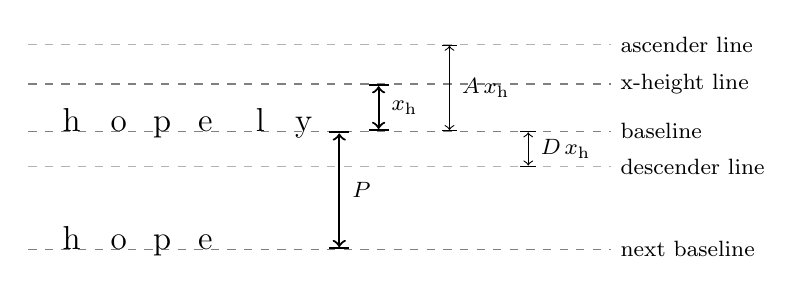
\begin{tikzpicture}[x=1cm,y=1cm,font=\footnotesize]
%% reference lines of the first text line
\draw[dashed,gray]      (0,0)    -- (7.4,0)    node[right,black]{baseline};
\draw[dashed,gray]      (0,0.6)  -- (7.4,0.6)  node[right,black]{x-height line};
\draw[dashed,gray!60]   (0,1.1)  -- (7.4,1.1)  node[right,black]{ascender line};
\draw[dashed,gray!60]   (0,-0.45)-- (7.4,-0.45)node[right,black]{descender line};
%% letters placed against those lines: h has an ascender, x and o do not, p descends
\node[anchor=base,font=\large] at (0.55,0) {h};
\node[anchor=base,font=\large] at (1.15,0) {o};
\node[anchor=base,font=\large] at (1.70,0) {p};
\node[anchor=base,font=\large] at (2.25,0) {e};
\node[anchor=base,font=\large] at (2.95,0) {l};
\node[anchor=base,font=\large] at (3.50,0) {y};
%% x-height dimension
\draw[|<->|,thick] (4.45,0) -- (4.45,0.6) node[midway,right=1pt]{$x_{\mathrm{h}}$};
%% ascender and descender reach, measured from the baseline in x-heights
\draw[|<->|] (5.35,0) -- (5.35,1.1)  node[midway,right=1pt]{$A\,x_{\mathrm{h}}$};
\draw[|<->|] (6.35,0) -- (6.35,-0.45)node[midway,right=1pt]{$D\,x_{\mathrm{h}}$};
%% second text line, to show the pitch
\draw[dashed,gray] (0,-1.5) -- (7.4,-1.5) node[right,black]{next baseline};
\node[anchor=base,font=\large] at (0.55,-1.5) {h};
\node[anchor=base,font=\large] at (1.15,-1.5) {o};
\node[anchor=base,font=\large] at (1.70,-1.5) {p};
\node[anchor=base,font=\large] at (2.25,-1.5) {e};
\draw[|<->|,thick] (3.95,0) -- (3.95,-1.5) node[midway,right=1pt]{$P$};
\end{tikzpicture}
\caption{The five quantities every subsystem measures handwriting against. The x-height $x_{\mathrm{h}}$ is the height of a lower-case letter with no tall part and no tail; an ascender reaches above it and a descender below the baseline. The ascender and descender reaches $A$ and $D$ are stored as multiples of $x_{\mathrm{h}}$, so $A>1$ and $D<0$. The line pitch $P$ is the baseline-to-baseline distance and is the unit used by this block; $x_{\mathrm{h}}$ is the unit used by every block after it.}
\label{fig:seg-geom}
\end{figure}

Ink is described in two tiers. A strict page-wide mask fixes the structure of the page, such as where the paper is and where the lines are. A second, more permissive threshold is then applied inside each individual crop, limited to a halo around that line's own strong ink, which recovers pale strokes that the strict mask missed. The reason for two tiers is that a threshold loose enough to catch a faint stroke is also loose enough to catch a shadow, so the loose threshold is only trusted next to ink that is already known to belong to that line.

The six stages are reduce, ink mask, deskew, clean-up, pitch and centres, and finally seams and crops. They are described in that order below, which is the order the data flows through them.

Three of the stages resample an image, and they do it by bilinear interpolation at the source position given by Equation~\ref{eq:seg-resize}. The exception is one ownership map, which uses nearest neighbour, because the values in that map are integer line indices and interpolating them would invent indices that do not exist. Equation~\ref{eq:seg-clf} is the scale used to paste a finished crop onto the white $640\times64$ canvas that both networks expect, flush left and vertically centred.
\begin{align}
y_s&=\frac{(i+0.5)\,h}{h'}-0.5,\quad x_s=\frac{(j+0.5)\,w}{w'}-0.5,\quad I'(i,j)=\sum_{a,b\in\{0,1\}}\omega_{ab}\,I(\lfloor y_s\rfloor+a,\lfloor x_s\rfloor+b),\label{eq:seg-resize}\\
s&=\min\!\Bigl(\frac{64}{h},\frac{640}{w}\Bigr),\qquad h'=\max(1,\mathrm{round}(hs)),\qquad w'=\max(1,\mathrm{round}(ws)).\label{eq:seg-clf}
\end{align}
The single scale factor $s$ in Equation~\ref{eq:seg-clf} is applied to both axes, so letter proportions are not distorted. Flushing the crop left has a second benefit that Section~\ref{sec:styleprofile} depends on: the map from a network time step back to a pixel column of the original crop is then the exact inverse $x_{\mathrm{orig}}=x_{\mathrm{canvas}}/s$, with no offset to track.

Each line record that the block returns holds the order index, the crop at native resolution, that canvas, and the bounding box in full-resolution coordinates. The block also returns page statistics: the chosen skew angle, the pitch, the paper coverage, the ink discarded off the paper, the straight pixels and artefact pieces removed, the line count and the wall-clock time. These allow a page to be checked after the fact without having to instrument the module.

\subsubsection{The three array primitives}

Almost every operation in this block is a sum, a maximum, or a test of whether anything is set, taken over a rectangular window. Computed directly, a window of radius $r$ costs $O(r)$ per pixel per axis. That is too slow here, because the illumination blur below uses a radius of up to 40 pixels.

The module therefore builds a summed-area table~\cite{crow1984}, also called an integral image, which is Equation~\ref{eq:seg-sat}. It is built in one $O(HW)$ pass of two cumulative sums, and after that the sum over a window of \emph{any} size costs four look-ups instead of $(2r+1)^2$ additions. The window corners are $y_2=y_1+2r+1$ and $x_2=x_1+2r+1$. The array is padded by $r$ using edge replication first, so that every window holds the same number of samples and a pixel near the border is not biased.
\begin{align}
S(y,x)&=\sum_{i<y}\sum_{j<x} I(i,j),\qquad
\mathrm{BoxSum}=S(y_2,x_2)-S(y_1,x_2)-S(y_2,x_1)+S(y_1,x_1),\label{eq:seg-sat}\\
\mathrm{AnyWithinRadius}&(m,r)[i]=\bigl[\,c[i+2r+1]-c[i]>0\,\bigr]=\Bigl[\textstyle\bigvee_{k=-r}^{r} m[i+k]\Bigr],\label{eq:seg-dilate}\\
\mathrm{LongRun}&(m,n)[j]=\bigl[\,\mathrm{ch}[h_j+1]-\mathrm{ch}[l_j]>0\,\bigr],\ l_j=\max(0,j-n+1),\ h_j=\min(j,L-n).\label{eq:seg-runmask}
\end{align}
The second primitive, Equation~\ref{eq:seg-dilate}, is a dilation. A square dilation separates into two one-axis dilations, and each of those is a cumulative sum of the mask followed by one subtraction, so it also costs the same at any radius. An erosion is then the complemented dilation of the complement, and a closing is a dilation followed by an erosion, which means no other structuring element has to be implemented.

The third primitive, Equation~\ref{eq:seg-runmask}, marks every pixel that lies on a run of at least $n$ consecutive set pixels. A run of length $n$ starts at position $i$ exactly when $c[i+n]-c[i]=n$, so the starts are found first and then a second cumulative sum marks every pixel covered by one. This is what stage~4 uses to find printed rules. Figure~\ref{fig:seg-primspseudo} gives all three primitives as pseudocode.

Only one true Gaussian filter is used in the whole block, and it smooths the row profile in stage~5. It is a 25-tap kernel $k[t]\propto\exp(-t^2/2\sigma^2)$ for $t=-12\ldots12$ with $\sigma=4$ rows, truncated at $3\sigma$ and normalised. Four rows is about a tenth of a typical pitch, so it smooths the ripple inside a line without blurring one line into the next.

\subsubsection{Stage 2: lighting normalisation and the ink mask}

The intensity measured by a camera is approximately the reflectance of the paper multiplied by the illumination falling on it. Because the unwanted term is a multiplication and not an addition, it is divided out rather than subtracted. The working grey image $G$ is divided by a single box mean of itself, which is Equation~\ref{eq:seg-flat}. The result is a ratio image $\rho$ which is close to 1 on paper whatever the lighting, and on ink is the ink-to-paper reflectance ratio of the pen itself.
\begin{align}
\rho(p)&=\frac{G(p)}{\max\bigl(\mathrm{BoxMean}_r(G)(p),\,1\bigr)},\qquad r=\max\bigl(8,\;\min(40,\;\mathrm{round}(H/41))\bigr),\label{eq:seg-flat}\\
t^*&=\arg\max_t\;\omega_B(t)\,\omega_F(t)\,\bigl[\mu_B(t)-\mu_F(t)\bigr]^2 .\label{eq:seg-otsu}
\end{align}
The radius $r$ in Equation~\ref{eq:seg-flat} scales with the image height, so the background estimate covers the same fraction of the page at any resolution. It must be much larger than a letter, otherwise the letters would darken their own background estimate and disappear.

Once the shading has been divided out, the ink decision is a single global threshold, and Otsu's method~\cite{otsu1979} is used to choose it. Otsu's threshold is the value that maximises the between-class variance of Equation~\ref{eq:seg-otsu}, where $\omega_B$ and $\omega_F$ are the fractions of samples below and above $t$ and $\mu_B$ and $\mu_F$ are their means. A pixel is marked as ink when $\rho<t^*$. The cumulative form of Equation~\ref{eq:seg-otsu} is evaluated for all 256 histogram bins at once rather than in a loop.

A single global threshold is only possible because of the division. This is the step that removed the long chain of clean-up filters that the project's first segmenter needed, and it is why this stage holds no tunable grey level at all. One extra test is still needed: a solid-area veto removes any window that is entirely ink, because no pen stroke fills a $9\times9$ window. That catches a binder shadow or the dark gutter of a bound book, which a global threshold would otherwise mark as ink. The whole stage is four array statements, given as pseudocode in Figure~\ref{fig:seg-inkpseudo}.

\subsubsection{Stage 3: deskew by searching rotations}

When the text lines are horizontal, the row-sum profile of the ink has sharp peaks at the line bodies and deep troughs between them. Any tilt smears those peaks, because a single row then cuts across several lines. The sharpness of the profile is therefore a measure of how level the page is, and it can be maximised directly.

A candidate angle is scored by the projection objective of Equation~\ref{eq:seg-skew}, in which $R_\theta$ is the ink mask rotated by $\theta$.
\begin{equation}
J(\theta)=\sum_y P_\theta(y)^2,\qquad P_\theta(y)=\sum_x R_\theta(y,x),\qquad \theta^*=\arg\max_\theta J(\theta).
\label{eq:seg-skew}
\end{equation}
Squaring the profile before summing is what makes Equation~\ref{eq:seg-skew} work. The total amount of ink does not change when the page is rotated, so $\sum_yP_\theta(y)$ is fixed and could not be used. The sum of squares is largest when the same ink is concentrated into the fewest rows, which happens when the lines are level.

The search is one sweep of 17 candidate angles from $-4^\circ$ to $+4^\circ$ in steps of $0.5^\circ$, scored on the stage-2 mask reduced by a further factor of two. There is no refinement pass, so the best accuracy the stage can reach is half a step, which is $0.25^\circ$.

The page is never actually rotated to score an angle, which is worth setting out because it is what makes the sweep affordable. Rotating a point by $\theta$ about the centre of the image puts it in row
\begin{equation}
k=(y-c_y)\cos\theta-(x-c_x)\sin\theta+c_y,
\label{eq:seg-skewrow}
\end{equation}
so the coordinates of the ink pixels can be mapped straight into row numbers by Equation~\ref{eq:seg-skewrow} and counted, which gives the profile $P_\theta$ of Equation~\ref{eq:seg-skew} without producing a rotated image at all. That is one pass over the ink pixels per angle instead of seventeen image rotations, measured at 31 times faster, and it avoids resampling the mask seventeen times, each of which would blur it slightly further and bias the comparison towards the angles evaluated last.

One detail of that counting is not optional. Ink that would fall outside the row range at a trial angle must be allowed to extend the profile rather than being clipped into the first or last row. Clipping piles every out-of-range pixel into a single row, and because the objective squares each row, that artificial spike scores higher than any real text line; it made the search choose an angle four degrees wrong on a tilted page before it was corrected.

Only once an angle is chosen is the page itself rotated, bilinearly, and the ink mask and ratio image are then recomputed, because Equation~\ref{eq:seg-flat} is not rotation-equivariant: rotating the page and then dividing does not give the same result as dividing and then rotating.

The first segmenter had a fault here that is worth recording, because the structure of the deployed stage prevents it. A sign mismatch between the rotation routine and the angle scorer meant the page was rotated the wrong way, which doubled the skew of every tilted page instead of removing it. The deployed module cannot have that fault, because the candidate masks are rotated by the very same call that is later applied to the page, so the two cannot disagree about the sign. Section~\ref{sec:seg-test} measures what the stage actually achieves.

\subsubsection{Stage 4: removing what is not handwriting}

A first pitch $P$ is computed by the procedure of stage~5, and every threshold in this stage is a multiple of it. Three kinds of nuisance are then removed in turn.

The first is the area outside the sheet. Handwriting disappears under a coarse enough average while the sheet itself does not, and that is what separates them. The working image is block-averaged down, blurred, and thresholded against its own median, after which the largest bright connected component is taken to be the sheet and is eroded slightly to keep its darkened rim out of the ink mask. The result is reported as \texttt{paperCoverage} and \texttt{inkOutsidePaper}.

The second is printed structure. Ruled paper, underlines and the spine shadow of a bound book weld separate text lines into one piece of ink, which would defeat the line separation entirely. What distinguishes them from handwriting is that they run straight for longer than a line spacing, and handwriting does not. The long-run primitive is therefore applied per axis, bracketed by a dilation and a re-intersection as in Equation~\ref{eq:seg-cand}, where $\mathcal D_r^{y}$ and $\mathcal D_r^{x}$ are one-axis dilations.
\begin{equation}
\begin{aligned}
\mathrm{flat}&=\mathcal D_{1}^{y}\Bigl(\mathrm{LongRun}^{x}\bigl(\mathcal D_{1}^{y}(\mathrm{ink}),\;\lfloor1.25P\rfloor\bigr)\Bigr)\wedge\mathrm{ink},\\
\mathrm{upright}&=\mathcal D_{3}^{x}\Bigl(\mathrm{LongRun}^{y}\bigl(\mathcal D_{3}^{x}(\mathrm{ink}),\;\lfloor1.4P\rfloor\bigr)\Bigr)\wedge\mathrm{ink}.
\end{aligned}
\label{eq:seg-cand}
\end{equation}
The dilation before the run test is what makes Equation~\ref{eq:seg-cand} tolerant of a slight tilt, because a rule that drifts by one row would otherwise break into runs too short to detect. The re-intersection with the ink mask afterwards means only real ink is ever removed, never the pixels the dilation added. The two run lengths, $1.25P$ horizontally and $1.4P$ vertically, are the essential point: both are longer than any single letter can be, so no letter can be mistaken for a rule.

The third kind of nuisance is edge slivers, corner shadows and fold creases, which survive the run test because they are not straight. These are judged as whole pieces instead of pixel by pixel, because what identifies them is a property of the whole shape, such as being long and thin or being sparse inside its own bounding box.

Doing that requires the ink to be grouped into pieces first, which is \emph{connected-component labelling}: every set pixel is given an integer label, and two pixels get the same label when a path of set pixels joins them. The mask is closed before labelling so that the pen lifts inside a word are bridged and a whole word becomes one piece rather than several. The labelling itself is done by a run-length union-find pass. Each row is first reduced to its horizontal runs of set pixels, which is far fewer objects than pixels, and a \emph{union-find} structure then records which runs have been found to belong together: it holds one representative per group and merges two groups in near-constant time when a run in one row is found to touch a run in the next. One pass over the rows therefore labels the whole page.

Every statistic used by the discard tests is then accumulated over the \emph{original} ink pixels rather than the closed mask, so the closing can join pieces but can never add area to a decision. Eight discard predicates are applied to each piece, combining its size, its aspect ratio, its faintness relative to the page's own threshold, and its distance from the frame. Table~\ref{tab:seg-artifact} in Appendix~\ref{sec:app-seg} states all eight with the nuisance each is meant to catch.

The most aggressive of the eight discards any piece whose leftmost ink lies within $\max(3,\lfloor0.5P\rfloor)$ of the left frame edge, whatever its size or darkness. This removes the facing page of an open book, but it also costs the first letters of a page photographed with no left margin, so the block requires a visible left margin.

\subsubsection{Stage 5: line pitch and line centres from the row-ink profile}

The row-ink profile is the count of mask pixels in each row, taken over a central window of the width so that the margins cannot contribute, and then smoothed with the Gaussian kernel described above. This is Equation~\ref{eq:seg-pitch}. A line centre is a peak of that smoothed profile, and a peak is an interior row that satisfies the three conditions of Equation~\ref{eq:seg-centres}.
\begin{align}
\mathrm{prof}(y)&=\sum_{x=\lfloor0.05W\rfloor}^{\lfloor0.97W\rfloor-1}\mathrm{ink}(y,x),\qquad \mathrm{sm}=\mathrm{prof}*k,\label{eq:seg-pitch}\\
&\mathrm{sm}(y)\ge\mathrm{sm}(y-1),\qquad \mathrm{sm}(y)>\mathrm{sm}(y+1),\qquad \mathrm{sm}(y)>0.06\max_u\mathrm{sm}(u).\label{eq:seg-centres}
\end{align}
The two comparisons in Equation~\ref{eq:seg-centres} are deliberately asymmetric, one using $\ge$ and the other $>$. If both used $\ge$, every row of a flat-topped peak would be reported as a separate line, and if both used $>$, a flat top would be missed entirely. As written, the last row of a plateau is taken exactly once. The third condition is a relative floor that rejects the small ripple between lines, and because it is a fraction of the strongest peak rather than an absolute count, it scales with the amount of ink on the page.

The pitch is the median of the gaps between consecutive peaks, which is used whenever at least two peaks exist. A median is used rather than a mean so that one unusually large gap, such as a paragraph break, cannot shift the pitch.

Three fallbacks follow in order, shown in Figure~\ref{fig:seg-pitchpseudo}. The first uses the \emph{autocorrelation} of the profile, which is the profile multiplied by a shifted copy of itself and summed, evaluated for every shift. That shift is called the lag. A profile made of evenly spaced line bodies agrees well with itself when shifted by exactly one line spacing, so the autocorrelation has a maximum at a lag equal to the pitch, and this holds even when the individual peaks are too weak to be detected one at a time. The mean is removed from the profile first, otherwise the overall amount of ink would dominate the sum at every lag. If fewer than two peaks were found, the pitch is therefore taken as the first maximum over lags 15 to $\min(200,L_{ac}/3)$ that reaches $0.7$ of the maximum in that range. It is only a fallback because the profile also agrees with itself at two line spacings, three, and so on, so the method can lock onto a multiple of the true pitch. If that also fails, the pitch is estimated from the letters themselves as $P=\max(15,\mathrm{round}(2.2\,\mathrm{median}\{h_c\}))$ over components with area $A_c\ge8$ and height $3\le h_c\le H$, where 2.2 is the measured ratio of pitch to letter height for these hands. If there are no usable components either, the pitch is set to 48 rows.

The pitch and the profile are recomputed on the cleaned mask after stage~4, because removing a rule or a shadow changes the profile. The peaks then become line centres through a greedy non-maximum suppression: peaks are taken in order of decreasing profile value, and a peak is accepted only if it lies at least $0.6P$ from every centre already accepted. That separation is more than half a pitch, so two genuine lines can never be merged into one.

\subsubsection{Stage 6: seams, pixel ownership and the line crops}

A straight cut halfway between two line centres would sever every descender and ascender that crosses it. The boundary between two lines must therefore bend around the ink. Between consecutive centres $c_0<c_1$ the module builds the cost field of Equation~\ref{eq:seg-cost2} and finds the cheapest path across it by dynamic programming over columns, which is Equation~\ref{eq:seg-seam}.
\begin{align}
C(y,x)&=4.0\,\tilde m(y,x)+0.012\left(\frac{y-\mu}{\max(1,(c_1-c_0)/2)}\right)^{\!2},\qquad \mu=c_0+\tfrac12(c_1-c_0),\label{eq:seg-cost2}\\
A(y,x)&=C(y,x)+\min_{|d|\le s}\bigl[\,A(y+d,\,x-1)+0.02\,|d|\,\bigr],\qquad A(y,0)=C(y,0),\qquad s=7.\label{eq:seg-seam}
\end{align}
In Equation~\ref{eq:seg-cost2}, $\tilde m$ is the closed ink mask and $\mu$ is the midline between the two centres, with the half-gap as the denominator so that the second term is dimensionless. The relative size of the two weights is the design decision. At 4.0 against a maximum of 0.012, crossing a single ink pixel costs more than three hundred times as much as sitting a half-gap away from the midline. The midline term therefore has no influence where there is ink, and only breaks ties over the blank gaps between words, where it keeps the seam from wandering far from where a line boundary belongs.

The recursion of Equation~\ref{eq:seg-seam} is exact, because the cost of a path is a sum over columns and every admissible predecessor is considered at each step. The step limit $s=7$ rows per column lets the boundary react quickly enough to dodge a tall narrow descender, and the penalty of 0.02 per row of displacement stops it zig-zagging where the cost is flat. The mask is closed before the cost field is built, because a plain dilation would inflate the strokes into blobs that the seam would then trace around instead of cutting between.

The two outermost boundaries are fixed rather than computed, at $\lfloor0.75P\rfloor$ beyond the first and last centre, which covers the ascenders of the first line and the descenders of the last. With that, $L$ centres give exactly $L$ bands. The whole computation is $O(15HW)$ at worst, which makes the seam search the most expensive single step in the block. Figure~\ref{fig:seg-seampseudo} gives the cost field and the recursion as pseudocode.

A band is not the same thing as a line of writing, because an ink pixel can lie in the wrong band. By default a pixel belongs to the band it lies in, the band index being the number of interior boundaries above it. Writing is not that tidy, so six correction rules act on top of that default, and each may only move a piece to an adjacent band or drop it. They return a cut-off tail to the band that holds most of its piece, place a small fragment by proximity, and follow an $i$ dot or an accent downwards to the stem it belongs to. The dot rule accepts a stem only when that stem's band also lies where an x-height band should sit below a dot, which is a much stronger test than either condition alone. The rules rest on each band's share of a piece's ink, where 0.15 counts as a genuine presence, and on the \emph{major} band, which is the topmost band reaching the piece, because a piece spanning two lines is the upper line's descender. Table~\ref{tab:seg-own} in Appendix~\ref{sec:app-seg} states all six, and every size in them is a multiple of $P^2$ so that no rule is tied to a pixel count.

The crops themselves are rendered from the full-resolution page, not from the working image. The half-resolution background estimate is enlarged by Equation~\ref{eq:seg-resize} and the full page is divided by it, so the recogniser receives every pixel the camera captured even though every decision was taken at half resolution. A band is emitted only if it carries enough owned ink over enough rows, which drops a band that holds nothing but a stray mark.

Each crop is composited from three layers. The first is the band's own ink mask, enlarged bilinearly, which gives a soft edge rather than a hard one. The second is a recovery mask, which is Equations~\ref{eq:seg-flat} and~\ref{eq:seg-otsu} applied again inside this crop alone, where a pale stroke is a much larger fraction of the local contrast than it was on the whole page. The third is the halo of the band's own strong ink.

The three are combined by a \emph{hysteresis} rule, Equation~\ref{eq:seg-hyst}. Hysteresis here means using two thresholds instead of one: a strict threshold marks pixels that are certainly ink, and a loose threshold is then allowed to add further pixels, but only where they are connected to something the strict threshold already accepted. This is the same principle used to link edges in edge detection, applied to ink rather than to edges. It is what makes the two-tier description of ink work, because a loose threshold on its own would accept shadows anywhere on the page, whereas a loose threshold restricted to the neighbourhood of known ink can only extend a stroke that is already there. The grey values are then stretched by Equation~\ref{eq:seg-stretch}.
\begin{align}
\alpha&=\max\Bigl(\alpha_{\mathrm{strong}},\ \ \mathbb 1[\rho_{\mathrm{local}}<t^*_{\mathrm{local}}]\cdot\alpha_{\mathrm{halo}}\cdot\mathbb 1[\text{not owned by another band}]\Bigr),\label{eq:seg-hyst}\\
\ell&=\mathrm{clip}\!\left(\frac{255\,(v-b)}{\max(w-b,1)},0,255\right),\qquad
\mathrm{out}=255\Bigl(1-\bigl(\tfrac{255-\ell}{255}\bigr)^{0.55}\Bigr).\label{eq:seg-stretch}
\end{align}
The two factors in Equation~\ref{eq:seg-hyst} do different jobs. The halo factor accepts a pale stroke only when it lies close to ink this line already owns, which is what stops the loose local threshold from importing a shadow. The ownership factor is an absolute veto, so two adjacent crops can never both claim the same ink. In Equation~\ref{eq:seg-stretch} the black point $b$ is the 40th percentile of the grey values under the mask rather than the darkest pixel, so a single dark speck cannot flatten the whole line, and the exponent of 0.55 lifts the mid-greys so that a faint stroke survives.

Outside the mask the crop is pure white. The crop is finally shifted horizontally so that its first inked column sits a fixed distance from the left edge, because the recogniser's input is left-flush by Equation~\ref{eq:seg-clf}.

\subsubsection{Testing the segmentation block}
\label{sec:seg-test}

Two properties of this block can be tested against a known answer, and both were measured on the 30 photographed pages of the five personal writers, at $2448\times3264$ pixels each. Table~\ref{tab:seg-test} gives the results.

The first is whether the block finds the right number of lines. The ground truth is the transcription that was typed by hand when each page was collected, so the number of non-empty lines in that file is the number of lines the page actually holds. The block found the correct number on all 30 pages, which is 669 lines in total with no page over-segmented or under-segmented. This also settles the relative floor of Equation~\ref{eq:seg-centres}, which was the one threshold in stage~5 with no evidence behind it: a line peaking below six per cent of the strongest would be lost silently, and over these 30 pages no line was lost.

The second is whether the deskew of Equation~\ref{eq:seg-skew} recovers a known tilt. One page per writer was rotated by a known angle, the stage was run on the rotated page, and the angle it chose was compared with the angle it should have chosen. Two sets of angles were used. Seven angles that are multiples of the $0.5^\circ$ search step were recovered exactly in all 35 trials. Four angles that fall between search steps were recovered to $0.25^\circ$ in all 20 trials, and $0.25^\circ$ is exactly half the step, which is the best any search on that grid can do. The stage is therefore limited by the coarseness of its own search grid and not by the objective, which is a useful thing to know: if better than $0.25^\circ$ were ever needed, the fix is a second refinement sweep and not a different measure of sharpness.

\begin{table}[h]
\centering
\fontsize{9}{11}\selectfont
\setlength{\tabcolsep}{4pt}
\begin{tabularx}{\linewidth}{|p{4.3cm}|p{3.3cm}|X|}
\hline
\textbf{Measurement} & \textbf{Result} & \textbf{What it shows} \\
\hline
Line count against the hand-typed transcription, 30 pages & \textbf{30 of 30} pages exact; 669 of 669 lines & The line separation is correct on every page tested, and the relative floor of Equation~\ref{eq:seg-centres} lost no line. \\
\hline
Deskew, 7 angles on the search grid, 5 pages & \textbf{35 of 35} exact & The objective of Equation~\ref{eq:seg-skew} picks the correct grid point every time. \\
\hline
Deskew, 4 angles between grid points, 5 pages & \textbf{20 of 20} at $0.25^\circ$ & The residual error is exactly half the search step, so the stage is quantisation-limited, not objective-limited. \\
\hline
Time per page, $2448\times3264$ & \textbf{4.9 to 9.7\,s}, mean 7.9\,s & The cost of the deployed module, which had not previously been measured. Measured with the project's own resampling throughout. \\
\hline
Measured line pitch $P$ & 47 to 58 pixels & The scale unit varies by 23\,\% across these writers, which is what the block is designed to absorb. \\
\hline
Chosen skew angle on the unrotated pages & $-1.5^\circ$ to $+3.0^\circ$ & Real photographs are tilted by more than a degree, so the stage is doing necessary work. \\
\hline
\end{tabularx}
\caption{Measured performance of the deployed segmentation block over the 30 photographed pages of the five personal writers. These are the pages the system was built on, not an unseen test set, so the line-count result shows that the block handles the material it was designed for and not that it generalises to new conditions.}
\label{tab:seg-test}
\end{table}

Two things must be said about what these figures do and do not prove. The 30 pages are the pages the system was built on, so the line-count result is not an unseen test; it shows that the block handles the material it was designed for. A fair test needs pages photographed under conditions not represented here, such as a different pen, a different room or a different camera. The deskew result is stronger, because the injected angle is ground truth that no part of the design could have been fitted to.

The timing figure also corrects an attribution. The 24.8 to 69.1\,s per page reported in Section~\ref{sec:results} is a timing of \texttt{SegmentPage.ProcessPage}, the retired segmenter, recorded in the stored field \texttt{stage1\_processpage\_s}. On the same page resolution the deployed module takes 4.9 to 9.7\,s, which is roughly five times faster, because it makes one pass over a half-resolution image where the retired module made four passes over a larger one. The mean of 7.9\,s is still about four times the two seconds that requirement R4 allows for capture and conditioning, so conditioning does not meet that budget, but it misses it by a factor of four and not by a factor of twelve. These figures are for the deployed code with the project's own resampling; the same module using the imaging library's compiled resampling took 2.8 to 8.4\,s, so writing the resampling in array arithmetic costs about 40\,\% of the block's run time, which is the price of the library-free claim and is stated rather than hidden.
\mustdo{update the segmentation figures of Section~\ref{sec:results} and of the R4 budget to the deployed module's 4.9 to 9.7\,s measured here, keeping the retired module's range only where it is explicitly labelled as such.}
\mustdo{time \texttt{SegmentLean.SegmentLines} on the ODROID N2+ over the same 30 pages; the project files hold no figure for the board, and the board is expected to be slower than the laptop these figures were taken on.}
\mustdo{produce the four figures cut for space: the four-panel lighting normalisation (photograph, grey, background, ratio) from \texttt{InkMask}, the skew objective $J(\theta)$ over the 17 angles, the paper region from \texttt{PaperRegionMask}, and the \texttt{\_cuts\_overlay.jpg} that \texttt{SegmentLean.py} already writes. Insert the last first if space is recovered.}

\subsubsection{Design alternatives and limitations}

Table~\ref{tab:seg-alt} sets the main design choices against the alternatives that were considered. The project's first segmenter, \texttt{SegmentPage.py}, was about 2200 lines and sixty functions against the eleven here. It resized every photograph to a long side of 2400 pixels, thresholded locally, removed printed structure in four passes, took a median glyph height as its scale unit, scored components for being diagrams, chained them into lines and deskewed each line separately. No part of the deployed pipeline calls it any more. Three of its capabilities were given up with it: diagram tagging, per-line deskew, and the wider $\pm8^\circ$ search at $0.1^\circ$. The first two are acceptable for plain prose pages and the third is covered by the test above.

With $N_p=HW$ the pixel count of the working image, which is a quarter of the photograph's, every pass is $O(N_p)$ except the seam search at $O(15N_p)$, which dominates, and the ownership rules, whose cost grows with the amount of writing rather than the page size.

The block assumes left-to-right writing in a single column of roughly horizontal lines. The following limitations follow from that design rather than from tuning, and each is a consequence of a choice made above.

Skew beyond $\pm4^\circ$ is not corrected at all, and up to $0.25^\circ$ always remains, as Section~\ref{sec:seg-test} measures. Two columns of text, or a diagram beside the text, produce profile peaks that belong to no single line, and because diagram tagging was given up, an untagged diagram is cut into line-shaped crops and read as nonsense. A line whose profile peak falls below six per cent of the strongest is lost silently, although no such line occurred in the 30 pages tested.

A blank page raises an exception rather than returning no lines, because the first seam indexes an empty list of centres, and the same happens when no piece is letter-like. The server should therefore reject such an image before calling the block. Any ink within $\max(3,\lfloor0.5P\rfloor)$ of the left frame edge is discarded whatever its size, so a visible left margin is required, and a deliberate division bar or strike-through is removed as though it were a printed rule.

Illumination that varies faster than the radius of Equation~\ref{eq:seg-flat} leaves one side of a hard shadow edge mis-thresholded. A dense diagram can darken its own background estimate until it disappears. A stroke thick enough to fill a $9\times9$ window is thinned by the solid-area veto. Page curl and perspective are untreated, a desk as bright as the paper defeats the paper region, and colour is treated like black ink because the module is monochrome throughout.

\begin{table}[h]
\centering
\fontsize{8.5}{10.2}\selectfont
\setlength{\tabcolsep}{4pt}
\begin{tabularx}{\linewidth}{|p{2.4cm}|X|}
\hline
\textbf{Decision} & \textbf{Alternatives, and why the deployed choice was made} \\
\hline
Lighting & Subtracting a blurred background leaves the contrast dependent on brightness. The nuisance is multiplicative, so dividing gives an ink-to-paper ratio that is independent of the lamp. A direct Gaussian, or three box means, also cost more than one box mean over a summed-area table. \\
\hline
Ink threshold & A local mean less an offset, or a local mean and standard deviation, marks something even in an empty region, because every region has a darkest pixel, and it has an offset in grey levels that must be tuned. After the division, one global Otsu threshold is enough, which is what removed the first segmenter's long chain of clean-up filters. \\
\hline
Scale unit & A median glyph height is upset by a heading in another size, and a fixed 2400\,px page throws away resolution. The pitch $P$ is the quantity the problem is posed in, and it is measured on the page itself. \\
\hline
Lines & Chaining components along a baseline curve needs a correct set of components first, so every clean-up error propagates into the line structure. It also took three passes, ten further constants and a quadratic merge. The row profile is one $O(N_p)$ pass and yields the pitch and the centres together. The accepted cost is one column only and no curved baselines. \\
\hline
Line boundaries & A straight cut at the midline severs every descender and ascender. The least-ink path bends around them and relaxes where there is no ink. \\
\hline
Skew & A Hough transform of the ink edges is dominated by ruled lines and diagram strokes. The projection objective is also the quantity stage~5 goes on to use, so it costs nothing extra. \\
\hline
Rule removal & A long morphological opening erases underlines and cannot follow a slope. Chaining fragments across gaps needs five constants, where the dilated long-run test needs two. \\
\hline
Not implemented & Text-versus-diagram tagging, per-line deskew and a four-point perspective warp are all absent. The first is accepted for plain prose pages, the residual drift is tolerated by the recogniser, and the camera looks straight down so the keystone distortion is small. \\
\hline
\end{tabularx}
\caption{Design alternatives of the deployed segmentation block. The last row records capabilities of the first segmenter that were deliberately given up.}
\label{tab:seg-alt}
\end{table}


\subsection{Text recognition}
\label{sec:textrec}

This subsection describes the neural network that decodes a handwritten line image into text (functional unit FU~2.3, requirement R2).
The recogniser follows the CNN-BiLSTM-CTC architecture of Kizilirmak and Yanikoglu~\cite{kizilirmak2023}, which was chosen because it was evaluated on the same public handwriting database used here~\cite{marti2002} and reports accuracies in the range that requirement R2 needs.
That paper describes an approach and a layer pattern rather than publishing code, so the network was built from its description: the layer pattern, the filter counts and the recurrent width are taken from it, while the input geometry, the data pipeline, the label cleaning, the augmentation and the staged training recipe were decided for this project.
No machine-learning library is used in the recogniser, in the writer classifiers of Section~\ref{sec:writerid} or in the forced alignment of Section~\ref{sec:styleprofile}, so the forward passes, the backward passes and the optimiser updates are all evaluated by code written for this project (Section~\ref{sec:textrec-numpynn}).

\subsubsection{Problem statement and design approach}

The input is one grey-scale image of a text line from the segmentation block (Section~\ref{sec:segmentation}); the output is the string that was written.
Three properties of handwriting fix the design: cursive characters are joined, so their boundaries cannot be located reliably and cutting the line into characters, as the proposal planned, would pass every cutting error into a wrong reading; the number of characters is unknown and has no fixed relation to image width; and the available training material gives line images with transcriptions, but not the position of every character.
The design that follows is a convolutional neural network (CNN) followed by a bidirectional long short-term memory (BiLSTM) network trained with connectionist temporal classification (CTC)~\cite{graves2006}: the convolutional layers give one feature vector per narrow vertical slice, the recurrent layers give every slice the context of the whole line, and the CTC loss allows training from the line transcription alone.
That hybrid of convolution and recurrence is the combination reported to improve feature extraction and contextual understanding together~\cite{kumar2024,ma2023}.

\subsubsection{Input pre-processing}

The input size is fixed at $64\times640$ pixels, which allows batching and a fixed sequence length and is smaller than the $100\times960$ of the published design, which cost about an hour per training epoch on a processor-only computer.
A crop of height $h$ and width $w$ is resized uniformly by Equation~\ref{eq:rec-resize}, using the bilinear rule of Equation~\ref{eq:seg-resize}, pasted onto a white $640\times64$ canvas left-aligned and vertically centred, then inverted and normalised by Equation~\ref{eq:rec-norm}, so paper becomes $-1$ and ink $+1$.
\begin{align}
s&=\min\!\Bigl(\frac{64}{h},\frac{640}{w}\Bigr),\qquad w'=\max(1,\mathrm{round}(ws)),\qquad h'=\max(1,\mathrm{round}(hs)),\label{eq:rec-resize}\\
x&=\frac{(1-p/255)-0.5}{0.5}=1-\frac{2p}{255}.\label{eq:rec-norm}
\end{align}
A plain stretch to the canvas was used first but distorted letter proportions, in one case a horizontal scale of 0.48 against a vertical 0.35.
The constant of Equation~\ref{eq:rec-norm} is fixed rather than per-image, so white padding cannot change the contrast statistics, and the left flush makes the map from a time step back to a pixel column the exact inverse $x_{\mathrm{orig}}=x_{\mathrm{canvas}}/s$ that Section~\ref{sec:styleprofile} needs.

\subsubsection{Network architecture}

Figure~\ref{fig:rec-arch} gives the stages with their tensor shapes, each verified for this project against the published pattern; the network holds 3\,358\,763 trainable parameters, of which the two recurrent layers hold 70.5\,\% and the third convolutional stage 24.2\,\%, and Table~\ref{tab:rec-layers} in Appendix~\ref{sec:app-rec} resolves that total layer by layer.

\begin{figure}[h]
\centering
\begin{tikzpicture}[x=1cm,y=1cm,scale=0.86,transform shape]
\tikzset{nb/.style={w2box,text width=2.55cm,minimum height=1.5cm}}
\node[nb] (in) at (-6.2,0) {\textbf{Input}\\ $1\times64\times640$};
\node[nb] (s1) at (-3.1,0) {\textbf{Stage 1}\\ 2$\times$[conv 3$\times$3, BN, ReLU], 32 ch.\\ $32\times64\times640$};
\node[nb] (p1) at (0,0) {\textbf{Max-pool 2$\times$2}\\ $32\times32\times320$};
\node[nb] (s2) at (3.1,0) {\textbf{Stage 2}\\ 4$\times$[conv, BN, ReLU], 64 ch.\\ $64\times32\times320$};
\node[nb] (p2) at (6.2,0) {\textbf{Max-pool 2$\times$2}\\ $64\times16\times160$};
\node[nb] (s3) at (6.2,-2.3) {\textbf{Stage 3}\\ 6$\times$[conv, BN, ReLU], 128 ch.\\ $128\times16\times160$};
\node[nb] (hm) at (3.1,-2.3) {\textbf{Height max-pool}\\ $128\times1\times160$\\ $\rightarrow$ 160 vectors};
\node[nb] (ls) at (0,-2.3) {\textbf{BiLSTM $\times2$}\\ hidden 256 per direction\\ $160\times512$};
\node[nb] (ln) at (-3.1,-2.3) {\textbf{Linear + log-softmax}\\ $160\times75$};
\node[nb] (dc) at (-6.2,-2.3) {\textbf{Greedy CTC decoding}\\ collapse repeats, delete blanks $\rightarrow$ text};
\foreach \a/\b in {in/s1,s1/p1,p1/s2,s2/p2,p2/s3,s3/hm,hm/ls,ls/ln,ln/dc} \draw[w2arr] (\a)--(\b);
\end{tikzpicture}
\caption{Architecture of the text recogniser, the layer pattern being that of Kizilirmak and Yanikoglu~\cite{kizilirmak2023}. Tensor shapes are channels $\times$ height $\times$ width for the convolutional part and time steps $\times$ features for the recurrent part; BN denotes batch normalisation.}
\label{fig:rec-arch}
\end{figure}


\paragraph{The convolutional layers.}
A convolution applies the same small learned filter at every position of its input~\cite{yahya2021}, which is Equation~\ref{eq:rec-conv}. In it, $k$ is the kernel size, $s$ is the stride, and $X_{\mathrm{pad}}$ is the input with $p$ rows and columns of zeros added on each side. Applying one filter everywhere is what makes the layer useful here: a stroke junction means the same thing wherever on the line it appears, so the filter that detects it should not have to be learned again for each position. With $k=3$, $p=1$ and $s=1$ the output has the same height and width as the input, so only the pooling layers change the tensor size and every shape in Figure~\ref{fig:rec-arch} follows from the two pools alone.
\begin{align}
Y[o,i,j]&=b_o+\sum_{c=1}^{C_{\mathrm{in}}}\sum_{u=0}^{k-1}\sum_{v=0}^{k-1}W[o,c,u,v]\;X_{\mathrm{pad}}[c,\,s\,i+u,\,s\,j+v],\label{eq:rec-conv}\\
Y&=\tilde W\,\mathrm{cols}+b\,\mathbf 1^{\top}.\label{eq:rec-im2col}
\end{align}
Equation~\ref{eq:rec-conv} is six nested summations, which is far too slow to evaluate directly in array arithmetic. The implementation therefore uses the \emph{im2col} rearrangement of Equation~\ref{eq:rec-im2col}. Every $k\times k$ patch of the input that a filter would see is copied out as one column of a large matrix, and the filter weights are reshaped into rows, so the whole convolution becomes a single matrix product. The result is arithmetically the same sum, agreeing with the direct form to about $10^{-13}$, but about ten times faster, because one large matrix product is handled far more efficiently than millions of small ones. The cost is memory: the patches overlap, so each input pixel is copied up to $k^2=9$ times and the largest such matrix in this network holds 47\,MB.

\paragraph{Normalisation, the nonlinearity and pooling.}
Every convolution is followed by batch normalisation and a rectifier, and each stage ends with a pooling layer. All three are needed, and for different reasons.

\emph{Batch normalisation}~\cite{ioffe2015} rescales each channel so that, over the current batch of training images, it has zero mean and unit variance, and then applies a learned scale $\gamma$ and shift $\beta$ so the layer can undo that rescaling if it needs to. This is Equation~\ref{eq:rec-bn}. The problem it solves is that the distribution of a layer's inputs drifts as the layers before it are updated, which forces a small learning rate to stay stable. Holding the distribution fixed allows a much larger learning rate, which is what makes a twelve-layer stack trainable at all on a processor-only computer.
\begin{align}
\hat x&=\frac{x-\mu_B}{\sqrt{\sigma_B^2+\varepsilon}},\qquad y=\gamma\hat x+\beta,\qquad\varepsilon=10^{-5},\label{eq:rec-bn}\\
a&=\frac{\gamma}{\sqrt{\sigma^2_{\mathrm{run}}+\varepsilon}},\qquad b=\beta-a\,\mu_{\mathrm{run}},\qquad y=a\,x+b.\label{eq:rec-bnfold}
\end{align}
The batch mean and variance of Equation~\ref{eq:rec-bn} only exist during training, because at inference a single line is classified on its own and there is no batch to average over. Running averages collected during training replace them, and because both are then fixed numbers, the whole operation collapses into the single multiply-and-add of Equation~\ref{eq:rec-bnfold}. The small constant $\varepsilon$ prevents a division by zero in a channel that happens to be constant. Folding the normalisation into an affine map this way means the deployed code evaluates one multiplication and one addition per element instead of a mean, a variance and a square root, and Section~\ref{sec:rec-board} confirms the two forms agree numerically.

\emph{The rectifier} is $\max(0,x)$~\cite{nair2010}, which simply replaces every negative value by zero. Some nonlinearity between layers is essential, because a stack of purely linear layers collapses into one linear layer however deep it is, and could then not represent a letter shape. The rectifier is used rather than a smooth function because its derivative is either 0 or 1, so it neither saturates nor shrinks the gradient as it is propagated back through twelve layers.

\emph{Max-pooling} takes the largest value in each $2\times2$ window with a stride of 2, which halves both axes and has no parameters to learn~\cite{ji2021}. It does two things: it discards three quarters of the positions, which is what keeps the network small enough to run on the target hardware, and it makes the features tolerant of a small shift, because moving a stroke by one pixel usually does not change which value in its window is the largest.

\paragraph{From a feature map to a sequence.}
At the end of stage~3 the feature map is 128 channels of 16 rows by 160 columns, and it has to become a sequence before a recurrent layer can read it. The 16 rows are collapsed by taking a maximum down each column, which is Equation~\ref{eq:rec-hmax}. A maximum is used rather than a mean because it records only \emph{whether} a feature occurs anywhere in that column and not how much of the column it fills, which is the right behaviour for handwriting: an ascender and a short letter should produce the same answer about which letter is present, even though they occupy very different fractions of the column height.
\begin{align}
z_t[c]&=\max_{i}F[c,i,t],\qquad t=1,\ldots,T=160,\label{eq:rec-hmax}\\
\ell_t&=W_oh_t+b_o,\qquad \log y_t^k=\ell_t^k-\log\sum_{j=0}^{74}e^{\ell_t^j}.\label{eq:rec-softmax}
\end{align}
The two pooling layers have each halved the width, so what is left is $T=160$ time steps, each covering four pixels of the $640$-pixel input. Equation~\ref{eq:rec-softmax} is the output layer. The linear map produces 75 raw scores per time step, called \emph{logits}, which are unbounded real numbers and not yet probabilities. The softmax function exponentiates them and divides by their sum, which forces them to be positive and to add to one, so they can be read as a probability per symbol. The logarithm of that quantity is computed directly in the form shown, rather than by taking a softmax and then a logarithm, because $e^{\ell}$ overflows for a moderately large logit while the subtracted form stays finite. The loss of Section~\ref{sec:rec-ctc} needs the logarithm in any case.

The 74 symbols are the 26 lower-case and 26 upper-case letters, the ten digits and twelve symbols (space and . , ; : ' " ! ? ( ) -). Class 0 is reserved for the CTC blank described below, which is why the head has 75 outputs for 74 symbols. Characters outside the set are removed from every label, and lines that become empty, or that exceed 120 characters and so indicate two lines merged into one, are dropped.

\paragraph{The recurrent layers.}
A plain recurrent network multiplies by the same weight matrix at every step, so over a long sequence the gradient either shrinks away or grows without bound, and the network forgets what it saw earlier. A long short-term memory cell~\cite{hochreiter1997} avoids this by holding a separate cell state $c_t$ that is carried forward by addition rather than by multiplication, as $c_t=f_t\odot c_{t-1}+i_t\odot g_t$ and $h_t=o_t\odot\tanh(c_t)$, where $\odot$ is element-wise multiplication. Three learned \emph{gates} control that state: the forget gate $f_t$ decides how much of the previous state to keep, the input gate $i_t$ how much of the new candidate $g_t$ to add, and the output gate $o_t$ how much of the state to expose as the step's output. Because the state passes through an addition rather than a repeated multiplication, a gradient can cross many steps without vanishing. All four gate pre-activations are produced by a single matrix product with $W_{ih}\in\mathbb R^{1024\times I}$ and $W_{hh}\in\mathbb R^{1024\times256}$ and then split into four blocks of rows, which halves the number of products per step (Figure~\ref{fig:rec-lstmpseudo}).

A \emph{bidirectional} layer runs a second, independent pass over the reversed sequence and concatenates the two outputs, $h_t=[\overrightarrow h_t;\overleftarrow h_t]\in\mathbb R^{512}$, so every time step is informed by the whole line rather than only by what came before it. This is necessary for joined handwriting, where the up-and-down strokes of u, n and m are nearly identical locally and can only be told apart from what follows them. Two such layers are stacked, with no dropout, following the published design.
These shapes cost $4.17\times10^9$ multiply--accumulates per line, $3.79\times10^9$ of them convolutional (Equation~\ref{eq:rec-macs}), so the convolutions dominate the arithmetic even though the recurrent layers hold most of the parameters, while the recurrence is what makes the network inherently sequential.


\subsubsection{Connectionist temporal classification}
\label{sec:rec-ctc}

The network produces a probability for each of 75 symbols at each of its 160 time steps, but the transcription of that line has perhaps 40 characters. There are therefore four times as many outputs as there are characters, and nothing in the training data says which time steps belong to which character. That missing information is the \emph{alignment}, and obtaining it by hand for every training line is exactly what makes character-level labelling impractical.

Connectionist temporal classification~\cite{graves2006} removes the need for an alignment by refusing to commit to one. Instead of scoring the single alignment that happens to be correct, it adds up the probability of \emph{every} alignment that would produce the right transcription, and trains the network to make that total large.

Two definitions make this precise. A \emph{path} $\pi$ assigns one symbol to every time step, where that symbol may be any of the 74 characters or a special 75th symbol called the \emph{blank}, which means ``no character ends here''. The \emph{collapse map} $\mathcal B$ turns a path into a string by first merging runs of the same repeated symbol and then deleting the blanks, so that
\[
\mathcal B(\text{{-}{-}hh{-}e{-}ll{-}ll{-}o})=\text{hello}.
\]
The blank is what makes a genuine double letter possible. Without it, the two l symbols of ``hello'' would merge into one when repeats are collapsed; with a blank placed between the two groups, the merge stops at the blank and both survive. This is the reason the output layer has 75 classes for 74 symbols.

Equation~\ref{eq:rec-ctcprob} is then the probability of one path, the probability of the transcription as the sum over all paths that collapse to it, and the loss, which is the negative logarithm of that probability so that maximising the probability becomes minimising a loss.
\begin{align}
P(\pi\mid x)&=\prod_{t=1}^{T}y_t^{\pi_t},\qquad p(y\mid x)=\!\!\sum_{\pi:\,\mathcal B(\pi)=y}\!\!P(\pi\mid x),\qquad \mathcal L_{\mathrm{CTC}}=-\ln p(y\mid x),\label{eq:rec-ctcprob}\\
\hat\pi_t&=\arg\max_k y_t^k,\qquad \hat y=\mathcal B(\hat\pi).\label{eq:rec-greedy}
\end{align}
The number of paths in Equation~\ref{eq:rec-ctcprob} grows exponentially with $T$, so the sum can never be enumerated. It is instead evaluated by a forward--backward dynamic programme~\cite{graves2006}, which costs only $O(TU)$ for a transcription of $U$ characters because every path must pass through one of $2U+1$ states at each step, so the paths can be summed state by state instead of one at a time. The same recursion also yields the gradient of the loss in closed form, as the difference between what the network predicted and what the alignment lattice expects, which means no derivative of the recursion itself ever has to be taken. That recursion, the three transitions it admits, and the logarithmic-domain arithmetic it needs to avoid numerical underflow over 160 steps are set out in Appendix~\ref{sec:app-rec}, because they determine the gradient but not the architecture.

CTC imposes one requirement on the data, which is that a valid path must exist at all. Since a blank may be needed between adjacent repeated letters, the number of time steps must satisfy $T\ge U$ plus one extra step for every such repeat. The label cap of 120 characters, which is $\lfloor160\cdot0.75\rfloor$, keeps every transcription far enough below $T=160$ for this to hold with margin.

At inference the alignment is still unknown, but it no longer matters, because only the string is wanted. The most probable symbol at each step is taken, repeats are merged and blanks are deleted, which is the best-path or \emph{greedy} decoding of Equation~\ref{eq:rec-greedy}, given as pseudocode in Figure~\ref{fig:rec-decodepseudo}. This is an approximation: it returns the most probable \emph{path}, whereas the most probable \emph{string} would require summing over paths again. No lexicon, language model or beam search is used anywhere, so nothing corrects a misspelling. The published design reaches its best error rate with lexicon-constrained decoding, which is not implemented here, so its headline figure is not a result this project can claim.



\subsubsection{Training data and splits}

Four data sets were used: lines cut from scanned database pages by this project's own segmentation block with labels generated by alignment, the public line-level IAM transcription set with its official partitions (6\,481 training, 976 validation and 2\,915 test lines after label cleaning), photographed pages of the personal writers split per page, and a ten-author hold-out used for evaluation only.
Table~\ref{tab:rec-data} in Appendix~\ref{sec:app-rec} states each split rule with the leakage it leaves, which matters because \emph{no} figure in this report rests on a split that is both writer-independent and labelled by hand: the public test partition is the closest and is the only set used for no decision.
The one defect worth stating here is that label quality, not the network, limited the early measurements --- correcting the evaluation labels alone raised the ten-author hold-out accuracy from 42.7\,\% to 89.4\,\%, which is why the recogniser was later trained on a public line-level set with clean labels~\cite{mamun2024}.
\emph{Augmentation} is the practice of distorting each training image slightly and differently every time it is used, so that the network sees many variations of a line instead of the same one repeatedly and cannot simply memorise it. Only the training images are augmented, never the validation or test images, since those must stay fixed for the comparison between epochs to mean anything. At most one of four geometric transformations is applied per image: a horizontal \emph{shear}, which leans the writing and so simulates a different slant; a small \emph{rotation}, which simulates a page not quite square to the camera; an \emph{elastic distortion}, which displaces each pixel by a small random amount drawn from a smoothly varying field, so that strokes bend and thicken locally the way a different hand would write them; and a \emph{perspective} distortion, which moves the four corners of the image independently and so simulates a camera not looking straight down. All four are chosen because each one mimics a variation that really occurs in this data, which is the test of whether an augmentation is worth applying. Their magnitudes are listed in Appendix~\ref{sec:app-rec}. No colour, contrast, noise or blur augmentation is used, and no synthetic pre-training data.


\subsubsection{Training procedure}

The loss is minimised by mini-batch gradient descent with the RMSprop update of Equation~\ref{eq:rec-rmsprop}~\cite{tieleman2012}, in which $g_t$ is the gradient at update $t$, $\lambda=10^{-5}$ a weight decay added to it, $v_t$ the running average of the squared gradient with smoothing $\rho=0.99$, $\eta$ the learning rate and $\epsilon=10^{-8}$; there is no momentum, and the per-parameter step suits the very different gradient magnitudes of convolutional and recurrent layers.
In the joint stage the global gradient norm is clipped at 5 by Equation~\ref{eq:rec-clip} and batches with a non-finite loss are skipped; a plateau schedule halves the learning rate after a number of validation checks without improvement, $\eta\leftarrow\max(0.5\,\eta,\eta_{\min})$.
\begin{align}
g_t&\leftarrow g_t+\lambda\theta_{t-1},\qquad v_t=\rho\,v_{t-1}+(1-\rho)\,g_t^2,\qquad \theta_t=\theta_{t-1}-\eta\,\frac{g_t}{\sqrt{v_t}+\epsilon},\label{eq:rec-rmsprop}\\
g&\leftarrow g\,\min\Bigl(1,\frac{5}{\|g\|_2}\Bigr).\label{eq:rec-clip}
\end{align}
Training ran in the four stages of Table~\ref{tab:rec-stages}, each motivated by a limitation of the previous one: the base stage reproduced the published recipe on lines cut by this project's own tools, where the labelling defect made the data noisy; the clean-label stage warm-started from it on the public set; and fine-tuning on the personal lines alone was rejected because it cut the general accuracy by about ten points, which is catastrophic forgetting, barely reduced by freezing the convolutions.
The joint stage therefore continues on both sets at once with a weighted sampler: each public line gets weight $(1-f)/n_T$ and each personal line $f/n_P$ with $n_T=6\,481$, $n_P\approx280$ and $f=0.20$, and $n_T$ indices are drawn per epoch with replacement, so about 1\,296 draws per epoch are personal and each personal line is seen about 4.6 times with fresh augmentation.
The checkpoint of the epoch with the largest $\min(\text{accuracy}_{\mathrm{public}},\text{accuracy}_{\mathrm{personal}})$ is kept, so that neither domain is sacrificed.

\begin{table}[h]
\centering
\fontsize{8.5}{10.2}\selectfont
\setlength{\tabcolsep}{4pt}
\begin{tabularx}{\linewidth}{|p{1.8cm}|p{1.4cm}|p{2.0cm}|X|p{3.2cm}|}
\hline
\textbf{Stage} & \textbf{Data} & \textbf{$\eta_0$, batch, epochs, clip} & \textbf{Schedule and selection} & \textbf{Checkpoint and character accuracy} \\
\hline
1 Base & own lines & $10^{-3}$, 16, $\le200$, none & halve after 5 stalls; stop after 15; up to 3 restarts from the best weights; best validation loss & best validation loss 1.06 per line \\
\hline
2 Clean labels & public set & $10^{-3}$, 16, $\le200$, none & as above, up to 8 restarts; best public validation loss & \texttt{hf\_best}: 93.87 / 91.60\,\% public validation / test \\
\hline
3 Personal & personal lines & $3\!\times\!10^{-4}$, 8, 60, 5 & halve after 5 stalls; best personal validation loss & \texttt{personal\_best}: 84.26 / 80.56\,\% public, 90.2\,\% personal --- rejected \\
\hline
3a Personal, convolutions frozen & personal lines & as stage~3 & as stage~3 & 85.87 / 82.62\,\% public, 88.5\,\% personal --- forgetting only slightly reduced \\
\hline
4 Joint & both, $f=0.20$ & $5\!\times\!10^{-4}$, 16, 30, 5 & halve after 4 stalls on the sum of both validation losses; best $\min$ of the two accuracies & \texttt{joint\_best}: 94.03 / 91.82\,\% public, 89.64\,\% personal \\
\hline
\end{tabularx}
\caption{The four training stages with the catastrophic-forgetting variant 3a, and the character accuracies measured on each stage's own checkpoint file. All stages use RMSprop (Equation~\ref{eq:rec-rmsprop}) with weight decay $10^{-5}$ and a minimum learning rate of $10^{-5}$ or $10^{-6}$. Checkpoint names abbreviate \texttt{paper\_cnn\_bilstm\_ctc\_*.npz}. None of these figures was measured on \texttt{paper\_cnn\_bilstm\_ctc\_scratch\_best.npz}, the file the deployed loader prefers.}
\label{tab:rec-stages}
\end{table}

Four text checkpoints exist and the quoted accuracies belong to three of them (Table~\ref{tab:rec-stages}).
The fourth, \texttt{paper\_cnn\_bilstm\_ctc\_scratch\_best.npz}, is the output of the from-scratch trainer of Section~\ref{sec:textrec-numpynn} and is the file the deployed system actually uses, because the loader prefers it over the joint checkpoint whenever it exists, which it does.
This matters for every accuracy here, because no accuracy of the from-scratch checkpoint is reported anywhere in this report: its training produced no log and its file holds no epoch number and no best validation score.
The honest position is therefore that the four-stage recipe and its accuracies describe the joint checkpoint, while the deployed path loads a later checkpoint of the same architecture whose accuracy has not been measured.
\mustdo{either evaluate \texttt{paper\_cnn\_bilstm\_ctc\_scratch\_best.npz} on the sets of Table~\ref{tab:rec-results} and quote its figures beside the joint ones, or name the single checkpoint being submitted and remove the other from the loader's search path.}
A sweep over learning rate, LSTM width, depth, convolution width, dropout and optimiser (14 configurations of 50 epochs) was programmed but no result file kept, so the deployed architecture is the published one and not an optimum found here; the joint stage's training log was not kept either.

\subsubsection{From-scratch forward-and-backward implementation}
\label{sec:textrec-numpynn}

One module, \texttt{NumpyNN.py}, implements from the defining equations the forward and the backward pass of every layer used here and by the writer classifiers of Section~\ref{sec:writerid} --- the convolution of Equation~\ref{eq:rec-conv} with its im2col form, batch normalisation in both forms, the rectifier, max-pooling and the two adaptive pools, a fully connected layer, dropout, the multilayer bidirectional LSTM and the CTC recursion --- plus the update of Equation~\ref{eq:rec-rmsprop}, the writer classifiers' AdamW~\cite{loshchilov2019}, the two schedules and the clip of Equation~\ref{eq:rec-clip}.
One shared training program calls it to build either the recogniser or a writer classifier, since the two share the convolutional backbone, and the same functions run in inference form in validation and on the board; Figure~\ref{fig:rec-trainpseudo} gives that training step as pseudocode, including the transpose at which the width axis of the feature map becomes the CTC time axis.
The claim is narrower than ``no external library at all'', which would not be true: \texttt{NumpyNN.py} imports nothing but \texttt{numpy}, while the data pipeline uses two SciPy image utilities and only two, \texttt{gaussian\_filter} and \texttt{map\_coordinates} for the elastic augmentation and \texttt{find\_peaks} for row-ink minima when database pages are cut, plus the imaging library for file reading; neither touches a weight, a gradient or an update.


The backward pass of each layer is the standard gradient result for that layer, published with the layer itself and not derived here; what this project contributes is that every one of them is written out and evaluated by its own code instead of being supplied by a framework.
Appendix~\ref{sec:app-rec} lists those gradients, Equations~\ref{eq:rec-relubw} to~\ref{eq:rec-linbw}, together with the two places where the risk lies in the implementation rather than in the algebra: the col2im scatter-add of the convolution, which must accumulate because one input pixel appears in up to nine patches, and the reversed direction of the bidirectional layer, whose incoming gradient must be reversed and whose returned gradient reversed back.
Both would be wrong silently --- the first keeps one contribution in nine, the second produces a gradient wrong only in time ordering --- and neither would disturb a falling loss curve.

Because no automatic differentiation tool is available to check them, every backward pass was verified against a central-difference estimate of the same gradient, Equation~\ref{eq:rec-gradcheck}, and accepted only when the relative difference of Equation~\ref{eq:rec-gradtol} stayed below $10^{-6}$.
Of the 78 configurations of layer variant and tensor, \textbf{77 passed}, with relative differences between $4.9\times10^{-12}$ and $1.4\times10^{-10}$, four to six orders of magnitude inside the tolerance; 2044 individual tensor elements were probed in double precision.
The protocol, the precautions taken at the kinks of the rectifier and the max-pool, and the per-element worst case are in Appendix~\ref{sec:app-rec}.

The one configuration that failed is a genuine defect, reported here rather than removed.
The CTC loss does not survive an empty label sequence: the blank-interleaved target then has one entry, while two of the arrays carrying the recursion are built with two entries regardless, so the routine raises a shape error instead of returning the loss.
The fault is confined to the lattice indexing and touches neither the transition rule nor the gradient; a single-character target and a repeated-character target, which exercises the forbidden skip, both pass.
Its practical effect is small, because a line with no transcription never reaches the trainer, but the function is not safe against one and the fault is listed in Section~\ref{sec:discussion}.

With no graphics processor and no vectorised automatic-differentiation engine, one training step of a batch of 16 real lines took tens of seconds on a laptop processor, the dominant cost being an un-vectorised convolution rather than the recurrent layers or the CTC loss.
Training is not run to convergence from a random initial condition at this speed: the program instead loads every tensor of an existing checkpoint whose shape matches, a warm start.


\subsubsection{Evaluation metrics and measured accuracy}

Accuracy is measured with the Levenshtein edit distance, computed by the dynamic programme of Equation~\ref{eq:rec-lev}, and reported as one minus a character error rate micro-averaged over all lines, Equation~\ref{eq:rec-cer}: the total edit distance over the total reference length, case-sensitive.
The word measure is a longest-common-subsequence recall and not $1-\mathrm{WER}$.
Both are defined in Appendix~\ref{sec:app-rec}, where it is also shown that Section~\ref{sec:results} averages a \emph{floored, lower-cased, per-line} accuracy instead, so the subsystem figures of this subsection and the qualification figures of Section~\ref{sec:results} are not computed identically and should not be differenced.

\begin{table}[h]
\centering
\fontsize{8.5}{10.2}\selectfont
\setlength{\tabcolsep}{4pt}
\begin{tabularx}{\linewidth}{|p{3.1cm}|p{2.7cm}|X|}
\hline
\textbf{Data set} & \textbf{Result} & \textbf{Status of the figure} \\
\hline
Public set, validation (976 lines) & 94.03\,\% character; WER 21.1\,\% & Used for model selection, therefore mildly optimistic. \\
\hline
Public set, test (2\,915 lines) & 91.82\,\% character; WER 26.7\,\%; 15.9\,\% of lines exactly right & Used for no decision; the cleanest figure for the general benchmark, with the partition caveats of Table~\ref{tab:rec-data}. \\
\hline
Personal crops, 669 correctly cut lines & 98.61\,\% character, 94.21\,\% word & Measured on crops confirmed to match the label count, so segmentation failures are excluded, and the writers appear in the fine-tuning data. This is the operating figure of Section~\ref{sec:results}, not an end-to-end page figure. \\
\hline
Personal crops, per writer & Best Owen 99.15\,\%, worst Thiya 96.46\,\% & 75 to 206 crops each; Thiya is the weakest hand for recognition. Full breakdown in Table~\ref{tab:res-perwriter}. \\
\hline
Ten personal photographed pages, full page pipeline including segmentation and label alignment & 61.21\,\% (CER 38.79\,\%, 3\,617 of 9\,324 characters) & Six unique pages (four listed twice); measured with an earlier recogniser, before the personal pages were used for fine-tuning. The only figure that exercises the complete page-to-text chain. \\
\hline
Recognition speed, 669 crops & 8.86\,ms per character, 353\,ms per line & Against the 25\,ms per character of R4, a margin of about 2.8 times on the development laptop. \\
\hline
\end{tabularx}
\caption{Accuracy of the text recogniser. The public-set figures and the full-page figure predate the final training and are retained because they are the only ones measured on an independent partition or through the complete chain; the 669-crop figure is the current operating point. The two public-set rows were measured on \texttt{paper\_cnn\_bilstm\_ctc\_joint\_best.npz}; no row was measured on \texttt{paper\_cnn\_bilstm\_ctc\_scratch\_best.npz}, the checkpoint the deployed loader prefers.}
\label{tab:rec-results}
\end{table}

Joint training kept the general accuracy while adding the personal writers, the test accuracy rising by 0.22 points over the clean-label stage, so the weighted sampler is justified.
The word error rate is about four times the character error rate, so roughly one word in four contains a character error and only about one line in six is entirely correct: greedy decoding without a lexicon leaves spelling errors uncorrected.
The gap between 98.61\,\% on correctly cut crops and 61.21\,\% through the complete page pipeline is the largest discrepancy in this report, but the comparison is not clean: the two figures used different recogniser versions and page sets, and the full-page pages were later fine-tuned on, so an unknown part of the 37-point difference is recognition improvement.
What can be stated is that the operating figure's crops were hand-checked whereas the full-page path has no such guarantee, so the difference bounds the combined effect of segmentation and label alignment from above and cannot be charged to recognition, which is 98.61\,\% given correct crops; splitting the two needs the full pipeline re-run with the current recogniser on unseen pages, as Section~\ref{sec:discussion} proposes.

\subsubsection{Inference on the single-board computer, and alternatives}
\label{sec:rec-board}

The single-board computer runs the eval-mode form of the same module, so no re-implementation was needed between training and deployment: each convolution is the matrix product of Equation~\ref{eq:rec-im2col} and batch normalisation the folded form of Equation~\ref{eq:rec-bnfold}.
Before that form was trusted it was cross-checked against the training-mode forward pass on the same weights with the statistics frozen: over 1358 real lines the top-1 agreement was 100.00\,\% with a maximum absolute logit difference of $7.6\times10^{-6}$.
Recognition measured 8.86\,ms per character and 353\,ms per line over 669 real crops, inside the 25\,ms per character of requirement R4 by about 2.8 times, with the model already resident in memory on the development laptop.
Timing on the ODROID N2+ was not measured, and its ARM processor is expected to be slower, so the margin should shrink on the target hardware.
\mustdo{measure the recognition time per line on the ODROID N2+; the project files hold none, and the proposal's budget may cover the whole classification step.}
Compiled replacements for the convolution and the LSTM exist but are not used: the compiled convolution was slower than the optimised matrix product, and the compiled LSTM 2.8 to 4.4 times faster.

Table~\ref{tab:rec-alt} compares the design with the alternatives considered; only the chosen design was built and measured, so the statements about the others are arguments.
It fits the four facts of the problem: an output sequence of unknown length (CTC), cursive strokes needing context from both sides (bidirectional recurrence), line transcriptions as the only labels (an alignment-free loss), and a model small enough to re-implement on the single-board computer.

\begin{table}[h]
\centering
\fontsize{8.5}{10.2}\selectfont
\setlength{\tabcolsep}{4pt}
\begin{tabularx}{\linewidth}{|p{3.1cm}|X|}
\hline
\textbf{Alternative} & \textbf{Argument for, and against} \\
\hline
Character segmentation and a per-character classifier & Simple network and the proposal's plan, but it needs a segmenter that works on joined letters, classification errors cannot be repaired by context, and it needs character-level labels the available data lack. \\
\hline
Line-level CNN-BiLSTM-CTC (chosen) & No segmentation below the line, alignment-free training from line transcriptions, context from both sides, a string as output, and 3.36 million parameters that a from-scratch implementation can run. Against: it needs line segmentation, greedy decoding leaves spelling errors, and CTC assumes independent steps. \\
\hline
Lexicon or language-model decoding & Repairs near-miss words and gives the lowest error in the published design, but needs a corpus and a decoder, and the technical vocabulary and symbols of these pages are largely out of vocabulary. Future work. \\
\hline
Deeper backbones with skip connections & Easier training of very deep networks, but the 12-layer network with batch normalisation trained well and larger models cost memory and time on the single-board computer. \\
\hline
Attention encoder--decoder or transformer & Strong accuracy on large corpora, but far more parameters, large pre-training data, slow autoregressive decoding that can skip or invent text, and hard to implement from scratch for the board. \\
\hline
Word-level recognition & Uses the lexicon directly, but needs word segmentation and a closed vocabulary and is poor for names, numbers and symbols. \\
\hline
\end{tabularx}
\caption{Alternatives to the line-level recogniser.}
\label{tab:rec-alt}
\end{table}


\subsection{Writer identification}
\label{sec:writerid}

This subsection describes the two neural networks that decide which of the thirteen stored writers wrote a line or a page (functional unit FU~2.3, requirement R2) and that judge how closely synthesised handwriting resembles a writer (requirement R1).
Both share the recogniser's convolutional backbone, whose layer pattern follows Kizilirmak and Yanikoglu~\cite{kizilirmak2023} and is not an architecture originated here; the pooling and classification head, the stroke normalisation, the aggregation rule, the two trainers and the inference code were written for this project.

\subsubsection{Why two classifiers were needed}

The task is closed-set: choose one of $K=13$ known writers from a line image, the eight database writers 150, 151, 152, 153, 384, 551, 552 and 588 and five personal writers whose pages were photographed for this project.
A classifier trained on raw grey-scale crops read real held-out lines at 99.78\,\% over 1358 lines but identified the writer of \emph{synthesised} output in only about 28\,\% of trials, because the plotter draws every stroke at one width and one pressure while real handwriting carries a thickness and an ink density that a convolutional network exploits readily when training lines are few, and such a judge predicts neither what the machine can draw nor how a reader recognises a hand, which is by geometry.
A second classifier was therefore trained on stroke-normalised crops (Section~\ref{sec:wid-strokenorm}), in which thickness is removed by construction: the ink classifier serves real photographed pages, the shape classifier the best-of-$N$ search of Section~\ref{sec:synthesis}.
Both have all 966\,445 parameters trained, the ink classifier from the recogniser backbone and the shape classifier end to end; an earlier configuration fitted only the 13\,645 parameters of the shape classifier's head on features of a frozen backbone, which was a training fault, superseded but still the subject of the fault analysis below.

\subsubsection{Architecture}

The crop is brought to the fixed $64\times640$ canvas and normalised exactly as for the recogniser (Equations~\ref{eq:rec-resize} and~\ref{eq:rec-norm}), then passed through the same 12-layer convolutional stack, which produces a feature map $F\in\mathbb R^{128\times16\times160}$. The recurrent layers are not used here. The recogniser needs them because reading text depends on the order the letters come in, whereas writer identity does not: a writer's slant and stroke habits are the same whatever the sentence says, so the sequence information would only add parameters and cost.

What the head has to do is turn that feature map into one decision for the whole line, which means the two spatial axes must be removed. This is done by \emph{pooling} twice, in Equation~\ref{eq:wid-pool}, and the two pools deliberately use different operations.
\begin{align}
m_{c,t}&=\max_{r=1,\ldots,16}F_{c,r,t},\qquad f_c=\frac1{160}\sum_{t=1}^{160}m_{c,t},\qquad f\in\mathbb R^{128},\label{eq:wid-pool}\\
h&=\mathrm{ReLU}(W_1f+b_1)\in\mathbb R^{96},\qquad z=W_2\,\mathrm{Drop}_{0.2}(h)+b_2\in\mathbb R^{K},\label{eq:wid-head}
\end{align}
In Equation~\ref{eq:wid-pool}, $c$, $r$ and $t$ are the channel, row and column of $F$. A \emph{maximum} is taken down the height, because the question there is whether a stroke pattern occurs anywhere in that column, which is the same reasoning as in the recogniser. A \emph{mean} is taken along the width, because the question there is how \emph{often} that pattern occurs along the line. A maximum along the width would answer only whether the writer ever made that stroke once, which a single accident of handwriting could satisfy, whereas the mean measures a habit. The result is a position-independent summary: 128 numbers saying how commonly each learned stroke pattern appears, with no record of where. That is the right representation for this task and the wrong one for reading text.

One consequence of the mean is worth stating, because it is an assumption the design makes. A short line is padded with white to fill the canvas, and that padding contributes zero-feature columns to the average, so a short line's feature vector is diluted towards zero compared with a full line's. This is accepted rather than corrected, on the grounds that it happens identically during training and during use, so the network learns to work with it.

Equation~\ref{eq:wid-head} is the head itself: one hidden layer of 96 units with a rectifier, then a linear layer producing one score per writer, $K=13$ here. \emph{Dropout} is applied between the two layers, which during training sets a random 20\,\% of the hidden values to zero on every step and rescales the rest. The purpose is to stop the head depending on any single hidden unit, because with only 63 to 184 lines per writer a small head can otherwise memorise individual training lines rather than learning the writer's hand. Dropout is active only during training and is skipped entirely at inference, where a deterministic answer is wanted. Together the two pools and two layers replace the recogniser's recurrent stack and CTC head, giving 966\,445 trainable parameters of which only 13\,645 belong to the head, so almost all of the capacity is the shared backbone. Table~\ref{tab:wid-layers} in Appendix~\ref{sec:app-wid} resolves that count, and Figure~\ref{fig:wid-forward} gives the deployed forward pass, which the trainer also runs for validation.

\paragraph{The training objective.}
The 13 scores $z$ produced by Equation~\ref{eq:wid-head} are logits, as in the recogniser, so they are turned into probabilities by a softmax and the network is trained to put as much probability as possible on the correct writer. The measure of how badly it is doing is the \emph{cross-entropy} loss, which is the negative logarithm of the probability assigned to the true class. It is used rather than, say, counting mistakes, for two reasons: it is differentiable, so it can be optimised by gradient descent, and it punishes confident errors far more than hesitant ones, because the logarithm goes to infinity as the probability of the true class goes to zero. Equation~\ref{eq:wid-ce} gives the softmax, the loss and the decision rule.
\begin{align}
p_k&=\frac{e^{z_k}}{\sum_{j=1}^{K}e^{z_j}},\qquad
\mathcal L=\frac1B\sum_{n=1}^B\Bigl[\log\sum_je^{z^{(n)}_j}-z^{(n)}_{y_n}\Bigr],\qquad\hat k=\arg\max_kp_k,\label{eq:wid-ce}\\
\frac{\partial\mathcal L}{\partial z^{(n)}_k}&=\frac{1}{B}\bigl(p^{(n)}_k-\mathbb 1[k=y_n]\bigr),\label{eq:wid-cebw}
\end{align}
Here $B$ is the batch size, $y_n$ is the true writer of sample $n$ and $\mathbb 1[\cdot]$ is the indicator function, which is 1 when its condition holds and 0 otherwise. The loss is written in the combined form shown rather than as $-\log p_{y_n}$ for the same numerical reason as the log-softmax of the recogniser: the exponential of a large logit overflows, while the subtracted form does not. No class weights and no label smoothing are used, so every writer and every line count equally.

The gradient of this loss is unusually simple, and Equation~\ref{eq:wid-cebw} is the whole of it: the predicted probability minus 1 for the correct class, and the predicted probability itself for every other class. It is taken with respect to the logits $z$ rather than the probabilities $p$, which avoids having to differentiate the softmax separately and avoids dividing by a probability that may be very close to zero. Equation~\ref{eq:wid-cebw} is where the backward pass begins, and from there the chain runs back through the head, the two pools and the backbone using the layer gradients of Section~\ref{sec:textrec-numpynn}.



\subsubsection{Stroke normalisation}
\label{sec:wid-strokenorm}

Stroke normalisation re-draws a line at a constant pen width proportional to its own letter height, so the thickness cue is identical for every writer and for synthesised lines.
On the full-resolution crop, before the resize, it applies six steps: Otsu binarisation~\cite{otsu1979} (Equation~\ref{eq:seg-otsu}); removal of ruled lines and underlines by the run-length test of Equation~\ref{eq:wid-rule}; the pixel x-height from the row ink profile $P(r)$ by Equation~\ref{eq:wid-xh}; closing of hairline breaks by a square element of side $\mathrm{clip}(\mathrm{round}(0.045h),2,4)$, components under 6 pixels being dropped; thinning; and re-inking at one width.
\begin{align}
&H_{\mathrm{run}}\ge\max(24,\lfloor1.1h\rfloor)\quad\wedge\quad V_{\mathrm{run}}\le\max(3,\lfloor0.12h\rfloor),\label{eq:wid-rule}\\
&x_h=\text{base}-\text{top},\qquad\text{or}\ x_h=\max(8,h/3)\ \text{if no valid band exists or}\ x_h<4 .\label{eq:wid-xh}
\end{align}
Here $h$ is the crop height and $H_{\mathrm{run}}$, $V_{\mathrm{run}}$ the horizontal and vertical ink-run lengths through the pixel, so a rule pixel crossed by a vertical stroke is kept, and the core band of Equation~\ref{eq:wid-xh} runs from the first to the last row with $P(r)\ge0.45\max P$, the dense band of the lower-case bodies.
The width is $w=\mathrm{clip}(\mathrm{round}(0.14\,x_h),2,9)$ with odd structuring-element side $k=2\lfloor w/2\rfloor+1$, independent of the scan resolution ($x_h=20$ gives $w=k=3$).
Thinning to a one-pixel centre line uses the iterative Zhang--Suen rule~\cite{zhang1984}, which deletes a pixel only when it has two to six ink neighbours and exactly one background-to-ink transition around its neighbour ring, so stroke topology survives; the skeleton is then dilated back to width $k$ (Figure~\ref{fig:wid-snorm} gives the six steps as pseudocode).
Slant, letter proportions, spacing and connection habits survive, and every input of the shape classifier passes through the same transform, so real training lines and synthesised test lines share one geometry-only distribution; the ink classifier does not use it.
The renderer draws at 0.085 x-heights and the judge re-draws at 0.14, and because the judge re-draws every input itself the two constants need not match.
\mustdo{a figure of the six steps on real lines: grey crop, Otsu mask with rules removed, core band with $x_h$, skeleton, re-inked line and final canvas, for one database and one personal writer. Source: apply \texttt{StrokeNormalize} to crops from \texttt{Data/Datasets/IAMpages10} and \texttt{Software/CNN/NOGIT/dylan}.}


\subsubsection{Training data, protocol and the training fault}

The thirteen writers, three more than the proposal requires, are the eight database writers at ten pages each, except where a page failed the crop-to-label check, and five personal writers photographed as the project progressed.
The stroke-normalised set holds 689 database-writer lines and 669 personal-writer crops, 1358 in all, split into 920 training and 123 validation lines, 63 to 184 per writer.
The two kinds are split differently: a database writer's last labelled page is held out whole, the intended closed-set task, giving 8 to 11 validation lines each, whereas a personal writer's lines are shuffled on a fixed seed and 15\,\% become validation lines, with the consequences recorded as items~1 and~2 of Section~\ref{sec:wid-faults}.
The recogniser's augmentation, at most one of shear, rotation, elastic and perspective distortion per image, was inherited untuned (item~3).
Both classifiers were trained with AdamW, the decoupled-decay form~\cite{loshchilov2019} of Adam~\cite{kingma2015}, and cosine annealing, implemented in the recogniser's own layer library from the defining equations (Equations~\ref{eq:wid-adamwmom} and~\ref{eq:wid-adamw} in Appendix~\ref{sec:app-wid}).
Two properties of that choice matter to the design rather than to the arithmetic: the weight decay sits in the update and not in the gradient, so every parameter shrinks by the same fraction regardless of how large its gradient happens to be, and the norm clip of Equation~\ref{eq:rec-clip} is applied \emph{before} the moment update, so that one clipped batch cannot contaminate the running averages for the many steps over which they decay.
The ink classifier ran at $\eta_0=10^{-3}$ for 20 epochs on batches of 16 images with the clip at 5; the superseded frozen-head run used $\eta_0=3\times10^{-3}$, 500 epochs, batches of 64 feature vectors, no clipping and only the 13\,645 head parameters on 3\,680 stored vectors, and is the configuration that reached 83.36\,\%.

A backbone holds 84 tensors, the convolution weight and bias and the five batch-normalisation arrays of each of the twelve convolutional units, and a tensor-by-tensor comparison shows that all 84 differ between the recogniser, the ink classifier and the shape classifier, so the three backbones are three distinct sets of weights.
For the ink classifier that is what full fine-tuning requires; for the shape classifier it contradicts the original frozen-backbone recipe, which was itself a training fault, because no augmentation was re-sampled between epochs and each line contributed the same four fixed feature vectors for all 500 epochs.
End-to-end training raised the shape classifier from 83.36\,\% to 93.67\,\% on the same 1358 real lines, where 118 of one writer's 148 lines had previously gone to a single neighbour, so the frozen-head figures describe the superseded model only.
Both trainers write every tensor into one plain array archive keyed by layer name, with no object serialisation.

\subsubsection{Page decisions, evidence and alternatives}

On a real photograph the ink classifier is applied to every line the segmentation block delivers and the line probabilities are averaged, Equation~\ref{eq:wid-aggr},
\begin{equation}
\bar p_k=\frac1N\sum_{n=1}^Np^{(n)}_k,\qquad\hat k=\arg\max_k\bar p_k,\qquad\text{confidence}=100\,\bar p_{\hat k}\ \%,
\label{eq:wid-aggr}
\end{equation}
with $N$ the number of detected lines; the writer, the confidence and all thirteen page probabilities return to the browser.
Lines carry equal weight, not weighted by length or confidence, because averaging resists a few confidently wrong lines better than a majority vote and uses all the probability mass, although the two were never compared.
For synthesised output each rendered sentence instead gives one softmax and the target writer's probability becomes one score in the best-of-$N$ search of Section~\ref{sec:synthesis}.

Table~\ref{tab:wid-results} lists the five measurements that motivated the design and the status of each; chance level for thirteen writers is 7.7\,\% and the qualification figures belong to Section~\ref{sec:results}.
Neither classifier is redundant: the same hand is identified at 99.78\,\% by one instrument and 93.67\,\% by the other, which is a property of the instruments and not of the handwriting.
The corrected shape classifier's errors are scattered, eleven of the thirteen writers scoring 98.9\,\% or above.

\begin{table}[!htbp]
\centering
\fontsize{8}{9.6}\selectfont
\setlength{\tabcolsep}{3.5pt}
\begin{tabularx}{\linewidth}{|p{3.1cm}|p{1.9cm}|X|}
\hline
\textbf{Measurement} & \textbf{Result} & \textbf{Status of the figure} \\
\hline
Ink classifier, 1358 real lines & 99.78\,\% & 689 database and 669 personal crops; the live server's classifier for photographs. \\
\hline
Shape classifier, same lines, fault corrected & 93.67\,\% & End-to-end training instead of a frozen backbone with a fitted head. \\
\hline
Shape classifier, same lines, before correction & 83.36\,\% & 118 of one writer's 148 lines went to a single neighbour. \\
\hline
Ink classifier on synthesised output & 28\,\% over 39 drawn lines & Cannot judge constant-width output; the reason the shape classifier exists. \\
\hline
Shape classifier on synthesised output & 89.7\,\% through G-code (13 writers, 3 sentences, best-of-8); 80.1\,\% at best-of-30 & Circular: the same classifier family selects the candidates (Section~\ref{sec:wid-faults}, item~6). \\
\hline
\end{tabularx}
\caption{Evidence for the writer classifiers. Chance level for thirteen writers is 7.7\,\%, and none of these are held-out test accuracies.}
\label{tab:wid-results}
\end{table}

Four alternatives were weighed and none built, so they are arguments and not measurements: hand-crafted features with nearest-profile classification, interpretable and already half-measured by the profile builder, but needing feature selection and weak when two hands agree in coarse statistics; contour-direction and allograph statistics~\cite{bulacu2007}, text-independent and strong for large writer sets but hand-built and less direct as a judge of constant-width output; metric learning and deep fragment networks, open-set and scalable to hundreds of writers but needing far more than the thirteen writers and about 1\,000 lines available; and pen-width augmentation of the ink classifier, which would avoid a second network but reduces rather than removes the cue the normalisation removes by construction, no ablation having been run.
A single network with a text head and a writer head was in fact tried: writer accuracy reached 98.9 to 100\,\% by epoch 20 while text accuracy stalled at 28 to 29\,\%, so separate single-task networks were adopted.
The classifiers run on the single-board computer with the recogniser's own layer functions, so the trainer's validation pass and the server's page pass are the same code and need only the gradient check of Section~\ref{sec:textrec-numpynn}.
\mustdo{execution time of one classifier pass on the ODROID N2+.}

\subsubsection{Known faults and limitations}
\label{sec:wid-faults}

\begin{enumerate}\setlength{\itemsep}{0pt}\setlength{\parskip}{0pt}
\item There is no untouched test set: the best-validation checkpoint is also the reported one, so the same 123 lines serve for selection and for reporting and one line is worth 0.81 percentage points. Table~\ref{tab:wid-results} does not hold held-out test accuracies.
\item A personal writer's training and validation lines share pages, pen, paper and session, which a line classifier can exploit, so the figure is inflated for 52 of the 123 validation lines; holding out whole personal pages is the mitigation that was not carried out.
\item The inherited augmentation was never tuned and distorts the cues being classified: $\pm0.6$ of shear is about $\pm31^\circ$ against measured writer slants of $-7.5^\circ$ to $+42^\circ$.
\item The confidence of Equation~\ref{eq:wid-aggr} is an uncalibrated softmax probability from networks trained to a near-perfect fit, so over-confidence is expected.
\item The deployed end-to-end run's settings, best epoch and epoch count were not recorded, for either set of stored weights.
\item The set is closed with no unknown-writer class, the validation sets are small, the personal writers' geometry cues may be confounded with the collection session, and the shape classifier is also an objective of the generator (Section~\ref{sec:synthesis}), so its verdict on synthesised output is not independent.
\item The server lets the shape classifier take the default checkpoint and the loader prefers a from-scratch name that does not exist, so the default resolves to the stroke-normalised weights, which is correct; running that trainer would silently change the judge.
\mustdo{either remove the unused first entry from the author-checkpoint search order or make the server name the stroke-normalised file explicitly, as it already does for the ink classifier, so that the judge cannot change model by accident.}
\item Writer owen remains a systematic error, 48 lost lines belonging to him alone, unsolved in Section~\ref{sec:dis-unsolved}.
\end{enumerate}


% ---- Writer 3 shared definitions (used by 3.6 - 3.10) ----
\tikzset{
  w3box/.style={draw,rounded corners=2pt,fill=gray!12,align=center,font=\footnotesize,minimum height=8mm,inner sep=3pt},
  w3dark/.style={draw,rounded corners=2pt,fill=gray!30,align=center,font=\footnotesize,minimum height=8mm,inner sep=3pt},
  w3store/.style={draw,fill=white,align=center,font=\footnotesize,minimum height=8mm,inner sep=3pt,double,double distance=1pt},
  w3io/.style={draw,rounded corners=6pt,fill=white,align=center,font=\footnotesize,minimum height=8mm,inner sep=3pt},
  w3dec/.style={draw,diamond,aspect=2.2,fill=white,align=center,font=\scriptsize,inner sep=1pt},
  w3arr/.style={-{Stealth[length=2.2mm]},thick},
  w3dash/.style={-{Stealth[length=2.2mm]},thick,dashed},
  w3group/.style={draw,dashed,rounded corners=4pt,inner sep=5pt},
  w3lab/.style={font=\scriptsize,inner sep=1.5pt}
}

\subsection{Style extraction and glyph library}
\label{sec:styleprofile}

This subsection describes how a writer's style is learned from photographs of that writer's pages and stored permanently (functional units FU~2.5 to FU~2.7; requirements R1 and R6).
Training a writer trains no network: a \emph{style profile} is one text file built once per writer, holding a library of that writer's own letter shapes, each reduced to a thin centre-line pen path called a \emph{glyph}, plus measured numbers such as slant, letter height, spacing and how often letters are joined, after which no page images and no networks are needed to write in that style.
The builder is an offline program written for this project which uses the recogniser of Section~\ref{sec:textrec} for inference only; its input is the line crops and transcriptions of Section~\ref{sec:segmentation}, ten pages each of the eight database writers with the last labelled page held out so that no evaluation text enters a profile, and the notebook pages of the five personal writers abhinav, dylan, owen, thiya and yeukita with 15\,\% of their lines held out.
It runs twelve stages in strict order, with no branch and no loop, and the subsections below take them in that order: a line crop and its transcript go to the recogniser for its 160 log-probability vectors; those are forced-aligned by Equation~\ref{eq:sty-viterbi}; the character territories are cut at thin low columns by Equation~\ref{eq:sty-cut}; the line is binarised, stripped of rules and thinned as a whole; the skeleton is traced into chains, spurs pruned and junctions re-joined; the chains are split at the territories and simplified; each is normalised to the x-height frame of Equation~\ref{eq:sty-norm}; the quality gates and the letter prior of Equation~\ref{eq:sty-prior} are applied; the surviving variants, the medoid and the denoised prototype are assembled; the style statistics are measured; and one JavaScript Object Notation profile per writer is written.

\subsubsection{Forced alignment: where is each character?}

To cut a letter out of a line, the builder has to know where that letter is. In joined handwriting a character has no visible boundary, and no per-character labels exist for any of the data, so the position has to be inferred. What is available is the transcript of the line and a recogniser that reads lines, and the two together are enough.

\emph{Forced alignment} is the name for using a trained recogniser backwards. Normally the recogniser is asked what the line says; here the answer is already known, and it is instead asked \emph{where} it saw each character of that known answer. The word ``forced'' refers to this: the alignment is constrained to produce the transcript that is known to be correct, so the recogniser is not permitted to decide that the line says something else. The output is an assignment of each of the $T=160$ time steps, each covering a 4-pixel slice of the line, to one character of the transcript.

The quantities involved are the transcript $y=(y_1,\ldots,y_U)$, its blank-augmented form $y'=(\varnothing,y_1,\varnothing,\ldots,y_U,\varnothing)$ of length $S=2U+1$, which is the same construction CTC uses, and the log-probabilities $\ell_t(k)=\ln y_t^k$ the recogniser produces.

The difference between this and the training loss is one operator. Where the CTC loss of Equation~\ref{eq:rec-alpha} \emph{sums} the probability over every alignment, because for training it does not matter which alignment was right, Equation~\ref{eq:sty-viterbi} takes the \emph{maximum} instead and keeps only the single most probable one, because here the alignment is precisely what is wanted. This is the Viterbi algorithm~\cite{viterbi1967}, and $\delta_t(s)$ is the log-probability of the best path that reaches position $s$ of $y'$ at step $t$:
\begin{equation}
\begin{split}
&\delta_1(1)=\ell_1(\varnothing),\quad\delta_1(2)=\ell_1(y'_2),\quad\delta_1(s)=-\infty\ (s>2),\\
&\delta_t(s)=\ell_t(y'_s)+\max\bigl\{\delta_{t-1}(s),\ \delta_{t-1}(s-1),\ \delta^{\mathrm{skip}}_{t-1}(s)\bigr\},\\
&\delta^{\mathrm{skip}}_{t-1}(s)=\begin{cases}\delta_{t-1}(s-2)&s\ge3,\ y'_s\ne\varnothing,\ y'_s\ne y'_{s-2},\\-\infty&\text{otherwise.}\end{cases}
\end{split}
\label{eq:sty-viterbi}
\end{equation}
Because the maximum replaces the sum, the path itself can be recovered. Each step records which of the three predecessors won, and following those \emph{back-pointers} backwards from the end gives the whole best path at a total cost of $O(TS)$. The path is started from whichever of the last character or the final blank ends with the higher score, and character $i$ then owns every step whose winning position is $s^*_t=2i$, the odd positions being the blanks between characters.

The alignment is only as trustworthy as the recogniser's reading of that line, so lines the recogniser never really read must be discarded before their letters enter the library. The measure used is the \emph{alignment confidence} $\mathrm{conf}=\frac1T\sum_t\ell_t(y'_{s^*_t})$, which is the mean log-probability along the chosen path. A line where the recogniser was confident at every step scores near zero, and one where it was guessing scores strongly negative. The threshold is relative rather than absolute: a line is dropped when its confidence falls below the 25th percentile of that same writer's lines, provided at least eight lines survive. A per-writer threshold is used because the absolute confidence depends on how well the recogniser handles that hand in the first place, so one fixed cut-off would discard almost everything from the most difficult writers. On writer 153 this discards 22 of 88 lines.

The recogniser input is left-aligned at the uniform scale of Equation~\ref{eq:rec-resize}, so a frame boundary converts back to a crop pixel exactly, by Equation~\ref{eq:sty-f2p},
\begin{equation}
x_{\mathrm{px}}(a)=\frac{640\,a}{T\,s},\qquad s=\min\Bigl(\frac{64}{h},\frac{640}{w}\Bigr),
\label{eq:sty-f2p}
\end{equation}
for a crop of $h\times w$ pixels, about 6 pixels per frame on a 980-pixel line.
The span a CTC model assigns to a character cannot be used directly as the letter's extent. A CTC network is free to emit a character at any one step inside its true extent and blanks elsewhere, and in practice it emits a narrow sliver that lags slightly behind the ink. The spans are therefore used only for their \emph{centres} $c_k$, which are reliable, and the provisional boundary between two characters is taken as the midpoint between consecutive centres, $\hat x_k=\tfrac12(c_{k-1}+c_k)$.

That midpoint is only an estimate, and cutting there would often fall in the middle of a letter. In joined writing the only place where one letter honestly ends and the next begins is the ligature, the thin connecting stroke between them, and a ligature has two measurable properties: it is \emph{thin}, carrying little ink in its column, and it is \emph{low}, sitting near the baseline rather than high in the x-height band. The cut is therefore moved to the cheapest such column within a radius $r$ of the estimate, by Equation~\ref{eq:sty-cut}:
\begin{equation}
\begin{aligned}
\mathrm{cost}(x)&=\mathrm{thin}(x)+1.15\,\mathrm{top}(x),\qquad r=\max\bigl(3,\mathrm{round}(0.5x_h)\bigr),\\
x^*&=\arg\min_{|x-\hat x_k|\le r}\Bigl[\mathrm{cost}(x)+0.6\,\frac{|x-\hat x_k|}{r}\Bigr],
\end{aligned}
\label{eq:sty-cut}
\end{equation}
The two terms of the cost are the two properties of a ligature. Here $\mathrm{thin}(x)$ is the smoothed column ink count divided by its own 60th percentile over the non-empty columns, so it is near 1 in a typical column and below 1 in a thin one, and dividing by a percentile of the line itself makes the measure independent of pen thickness. The term $\mathrm{top}(x)$ is the highest ink in that column above the baseline, measured in x-heights and limited to 3, which is large in a column containing an ascender and near zero in a column containing only a low connecting stroke. The weight of 1.15 on $\mathrm{top}$ makes height slightly more important than thinness, because a thin column high up is more likely to be the upstroke of a tall letter than a ligature. The cost is forced to zero in a column with no ink at all, since a genuine gap between two unjoined letters is always the best possible cut. The final term in $x^*$ is a penalty proportional to the distance moved, which keeps the cut near the aligned estimate when no column in range is clearly better than its neighbours. The quantity $x_h$ is the x-height of Equation~\ref{eq:wid-xh}.

Two implementation points matter. The boundaries are written into one shared array and forced to be strictly increasing, because snapping each boundary independently can move two neighbours onto the same column and leave a character with no columns at all. Figure~\ref{fig:sty-code} gives the alignment and the cut cost as pseudocode.

The cuts are vertical, not along the writer's slant, and this was a measured decision rather than an obvious one. A slanted cut follows the natural geometry of a slanted hand and seems the better choice, but glyphs cut that way do not retile cleanly when reassembled at different spacings, because each one carries a sheared edge that only matches its original neighbour. Cutting along the slant lowered writer identification of the synthesised output from 81.8\,\% to 68.6\,\%, so vertical cuts were kept.


\subsubsection{From ink to ordered pen paths}

Each line is binarised and thinned by the very functions of Section~\ref{sec:wid-strokenorm} --- the Otsu threshold~\cite{otsu1979}, the rule removal of Equation~\ref{eq:wid-rule}, the closing, the speck removal, the core band of Equation~\ref{eq:wid-xh} for the baseline and x-height, whose median over the thirteen writers ranges from 15 to 47 pixels, and the Zhang--Suen thinning~\cite{zhang1984} --- the builder importing them from the same module as the classifier.
Two things differ.
The builder keeps the one-pixel skeleton instead of re-inking it, so the constant pen width of 0.14 x-heights and its clip to 2 to 9 pixels belong to the classifier path alone; and it thins the whole line \emph{once}, before the territory cuts of Equation~\ref{eq:sty-cut} are applied to the traced centre lines, because thinning each slice separately creates a spurious spine along the cut.
The \emph{slant} is the shear that makes the strokes vertical, scored by Equation~\ref{eq:sty-slant} on the column histogram of ink pixels $(x_i,y_i)$ sheared by a trial angle $\theta$ about their mean row $\bar y$, $y$ downwards,
\begin{equation}
x'_i(\theta)=\bigl\lfloor x_i-(y_i-\bar y)\tan\theta\bigr\rfloor,\qquad H_\theta(c)=\#\{i:x'_i(\theta)=c\},\qquad S(\theta)=\sum_cH_\theta(c)^2 ,
\label{eq:sty-slant}
\end{equation}
with $\hat\theta=-\arg\max_\theta S(\theta)$ over $\theta\in\{-45^\circ,-43.5^\circ,\ldots,45^\circ\}$, forward lean positive; $\sum_cH_\theta(c)$ being fixed, the score peaks when the ink falls in the fewest columns.

A thinned image is a picture of the pen path and not yet an ordered path, and four geometric operations recover the ordering, each resting on the 8-neighbourhood degree of a skeleton pixel (Equation~\ref{eq:app-degree}): a pixel of degree one is a stroke end, of degree two an interior point, and of degree three or more a junction.
The skeleton is \emph{traced} into chains grown from each unvisited end or junction through interior pixels only, so that every skeleton pixel belongs to exactly one chain; stopping at a junction rather than choosing a branch there is what makes the decomposition unique, a junction being precisely the point at which the true pen order cannot be recovered from the image.
Short false branches left by thinning are \emph{pruned} as spurs when a chain is both shorter than 2.5 pixels and has a free end (Equation~\ref{eq:app-spur}); the conjunction is necessary, because a short chain between two \emph{two} junctions is the crossbar of an A or the waist of an e and must be kept.
Because a self-crossing stroke such as the loop of an e breaks into several chains at the junction where it crosses itself, although the pen never lifted, chain ends within 1.5 pixels are \emph{re-joined} when their outward directions are nearly opposed, the continuation test of Equation~\ref{eq:app-rejoin}, which admits the curvature a pen shows through a crossing but rejects a genuine corner.
A chain crossing a territory boundary is then split, each crossing setting $\mathrm{connL}_i$ and $\mathrm{connR}_i$ to record that the pen did not lift.
Finally each chain is \emph{simplified} by the Douglas--Peucker recursion at $\varepsilon=0.6$ pixels, 0.05 to 0.12\,mm at 4\,mm per x-height, taken from~\cite{teikari2016} where it serves the same pen-path purpose, which bounds the deviation of the stored path from the traced one by $\varepsilon$ everywhere; a closed chain must be split at its farthest vertex first, since the recursion measures distance to the line through the two ends and would otherwise collapse a loop to two points.
Appendix~\ref{sec:app-syn-trace} states all four criteria as explicit conditions, with the resampling and smoothing that remove the lattice staircase thinning leaves behind.
Equation~\ref{eq:sty-norm} then maps every simplified point $(x,y)$ of a chain in the territory $[L,R)$ into a writer-independent frame with baseline 0, $y$ up, unit x-height and the slant removed:
\begin{equation}
y_n=\frac{y_b-y}{x_h},\qquad x_n=\frac{x-L}{x_h}-\sigma\,y_n,\qquad\sigma=\tan\hat\theta .
\label{eq:sty-norm}
\end{equation}
The synthesiser applies the inverse shear of Equation~\ref{eq:syn-place}, so glyphs are stored upright and re-appear at the writer's lean.
On a side confirmed connected the outward-running low connector is trimmed, and only if 18\,\% of the glyph width remains, the entry and exit points being recorded for the synthesiser's own connector.

\subsubsection{Variants, quality gates and the cross-writer letter prior}

Of about 2\,122 to 4\,031 raw instances per writer roughly 10\,\% survive five gates applied per character in order: geometry, outliers, the cross-writer prior of Equation~\ref{eq:sty-prior}, consensus against that writer's other instances of the same letter, and typicality, which keeps the best 12.
The cascade is ordered cheapest-first and most-local-first, so that a glyph is compared with its peers only once it is known to be a plausible letter at all; Appendix~\ref{sec:app-syn} states the test each gate applies and the thresholds it uses.

The hardest gate to design is the third, because it has to decide whether a letter is malformed, and one writer's ten pages do not contain enough examples to say what a well-formed letter looks like. Thirteen writers together do, and that is the idea the gate rests on: whatever all thirteen hands agree on must be the letter itself rather than any one writer's style.

To compare shapes they must first be reduced to numbers. Each glyph is turned into a \emph{shape descriptor} $v_g$, which is built by laying a $12\times12$ grid over the glyph's bounding box and counting how much stroke falls in each cell, giving 144 numbers. Three steps follow. The counts are \emph{damped} by taking a power below one of each, so that one cell holding a dense loop cannot dominate the comparison. They are then blurred slightly across neighbouring cells, so that a stroke falling a fraction of a cell either side of a boundary does not change the descriptor abruptly. Finally the whole vector is scaled to unit length, which removes the overall amount of ink and leaves only its distribution, so that a thick pen and a thin pen give the same descriptor for the same shape.

The reference shape $\bar v_c$ for character $c$ is the element-wise median of those descriptors over all thirteen writers, also scaled to unit length. A median is used rather than a mean so that one writer with an unusual letter form cannot pull the reference towards it. Because both vectors have unit length, their dot product is the cosine of the angle between them, which is 1 for identical distributions and smaller the more they differ. The distance of a glyph from the cross-writer reference is therefore
\begin{equation}
\mathrm{priorD}(g,c)=1-v_g\cdot\bar v_c\in[0,1],
\label{eq:sty-prior}
\end{equation}
and the 70\,\% of each writer's variants with the smallest $\mathrm{priorD}$ are kept. The important property of Equation~\ref{eq:sty-prior} is the direction in which it is used. It only ever \emph{rejects} one of the writer's own variants; it never substitutes a shape taken from another writer, so no part of another person's handwriting can enter a profile through this gate.

What Equation~\ref{eq:sty-prior} measures is how \emph{typical} a shape is, and Section~\ref{sec:sty-faults} records the limitation that follows from this: typicality is not the same thing as legibility, and a writer whose letters are consistently unusual scores badly on a prior built from everyone else.

Two further glyphs are derived per character and stored alongside the variants. The \emph{medoid} is the one real variant whose total distance to all the other variants of that character is smallest, so it is the writer's most representative actual letter. A medoid is used rather than an average because an average of several curves is not itself a pen stroke, whereas a medoid is a real example the writer really wrote. The distance is measured as the sum of absolute differences between descriptors, which is the $L_1$ norm, chosen because it is less affected by one wildly different variant than a sum of squares would be. The \emph{denoised prototype} is the per-stroke median curve of the largest group of variants sharing the same stroke count, and it is prepended to the list only when it is clearly cleaner than the variants it summarises (Figure~\ref{fig:sty-glyphs}). The medoid is also what Section~\ref{sec:synthesis} uses as the \emph{anchor}, the legible stand-in drawn when a writer's own variant is judged too malformed to use.

\begin{figure}[!htbp]
\centering
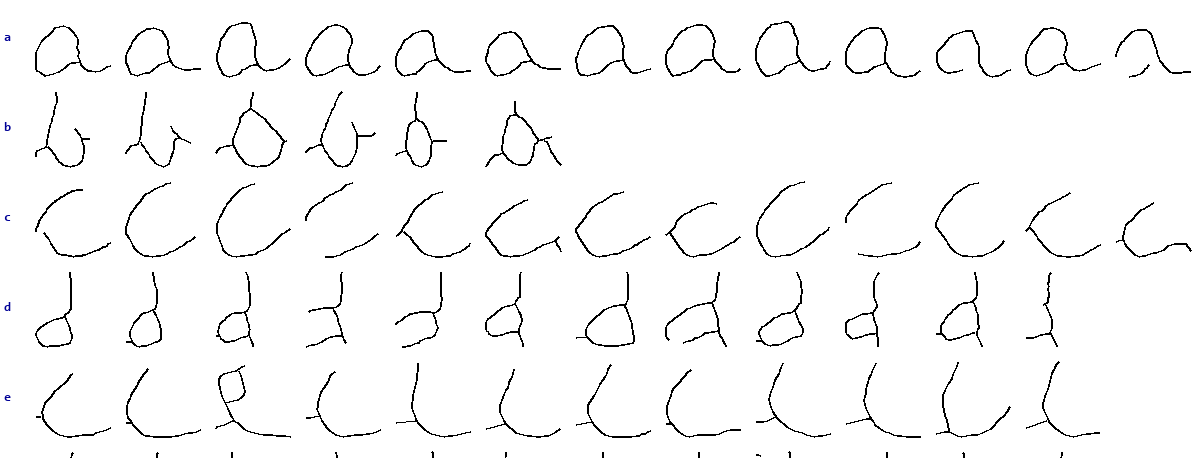
\includegraphics[width=0.78\linewidth]{Figures/w3_glyphs153_ae.png}
\caption{Stored variants of the letters a, b, c, d and e of writer 153, a strongly joined hand; each row is one character with up to 12 variants, and the short tails at the sides are remains of ligatures.}
\label{fig:sty-glyphs}
\end{figure}

\subsubsection{Style statistics and permanent storage}

Besides glyphs the profile holds numbers measured over the kept lines, every key of which is listed with an example as Table~\ref{tab:sty-schema} in Appendix~\ref{sec:app-syn}; two are not simple medians, the \emph{connectedness} being the adjacent letter pairs whose $\mathrm{connR}$ flag was set over all adjacent pairs, so its numerator counts the pen-down crossings recorded during tracing, and the word gap being the median of ink-free column runs wider than $0.5x_h$ on the \emph{real} ink, because CTC gives a space only a narrow slice.
Table~\ref{tab:sty-writers} shows how widely the thirteen differ --- slant $-10.5^\circ$ to $42.0^\circ$, connectedness 0.195 to 0.968, word gap 0.94 to 2.68 x-heights --- which is the diversity requirement R1 asks the system to reproduce; the thirteen files total about 4.8\,MB and load when the server starts (Section~\ref{sec:system}), which with the web interface listing them is requirement R6.
\mustdo{the demonstration of R6 (display of the stored writers, reproduction in a writer chosen by the examiner) and the storage device holding the files.}


\begin{table}[!htbp]
\centering
\fontsize{7.5}{9}\selectfont
\setlength{\tabcolsep}{2.5pt}
\begin{tabular}{|l|r|r|r|r|r|r|r|r|}
\hline
\textbf{Writer} & \textbf{Lines} & \textbf{Slant ($^\circ$)} & \textbf{$x_h$ (px)} & \textbf{$A$} & \textbf{$D$} & \textbf{Gap} & \textbf{Conn.} & \textbf{$\lambda$} \\
\hline
150 & 61 & $-4.5$ & 47 & 1.58 & $-0.72$ & 1.33 & 0.343 & 0.90$^\dagger$ \\
151 & 58 & 33.0 & 22 & 2.69 & $-1.09$ & 1.59 & 0.968 & 1.00$^\dagger$ \\
152 & 59 & 19.5 & 46 & 1.48 & $-0.79$ & 1.47 & 0.715 & 0.45$^\dagger$ \\
153 & 66 & 30.0 & 33 & 1.59 & $-1.10$ & 1.59 & 0.961 & 0.45$^\dagger$ \\
384 & 54 & 4.5 & 43 & 1.93 & $-0.71$ & 1.37 & 0.500 & 0.30$^\dagger$ \\
551 & 58 & 42.0 & 20 & 1.84 & $-0.67$ & 2.68 & 0.557 & 1.00$^\dagger$ \\
552 & 47 & $-10.5$ & 32 & 1.62 & $-0.56$ & 1.53 & 0.609 & 0.00$^\dagger$ \\
588 & 58 & 0.0 & 29 & 1.73 & $-0.68$ & 2.07 & 0.668 & 0.30$^\dagger$ \\
abhinav & 130 & 6.0 & 28 & 1.78 & $-0.84$ & 2.13 & 0.789 & --- \\
dylan & 79 & $-6.0$ & 26 & 1.68 & $-0.62$ & 1.79 & 0.195 & 1.00$^\dagger$ \\
owen & 93 & 0.0 & 32 & 1.51 & $-0.68$ & 1.10 & 0.319 & --- \\
thiya & 48 & 30.75 & 15 & 2.24 & $-1.00$ & 1.65 & 0.962 & --- \\
yeukita & 74 & 0.0 & 27 & 1.45 & $-0.58$ & 0.94 & 0.417 & 0.15$^\dagger$ \\
\hline
\end{tabular}
\caption{Scalar values of the thirteen stored style profiles, read directly from the files in \texttt{Software/CNN/NOGIT/StyleProfiles10}: kept lines, slant, pixel x-height, ascender $A$, descender $D$ and word gap (x-heights), connectedness and legibility parameter $\lambda$. Writers 150 to 588 are database writers, the last five personal. $^\dagger$The $\lambda$ column is \emph{not} read from these files, in which \texttt{legibilityLambda} is absent; it is the output of an earlier tuning run, as item~3 of Section~\ref{sec:sty-faults} records.}
\label{tab:sty-writers}
\end{table}

\subsubsection{Design alternatives and justification}

Character boundaries could have come from fixed widths, projection minima or hand labelling, but joined letters have no gaps and hand labelling of about 90 pages is impractical, while the recogniser already knows the text; several variants per letter are kept rather than one averaged letter, because averaging blurs letters whose strokes are arranged differently; and a generator learned from on-line pen data was not possible, since no such data exist for the thirteen writers, who contribute 47 to 130 usable lines each, and the pen path has to be recovered from the image in any case.
\mustdo{a figure of the builder stages on real lines: grey crop, ink mask with rules removed and core band, skeleton, traced chains in colour with the territory cuts as vertical lines, and one extracted glyph in the normalised frame, for one database and one personal line.}

\subsubsection{Known faults and limitations}
\label{sec:sty-faults}

\begin{enumerate}\setlength{\itemsep}{0pt}\setlength{\parskip}{0pt}
\item \emph{The builder cannot at present extract glyphs from a page image.} \texttt{ExtractLineGlyphs} of \texttt{BuildStyleProfile.py} opens with \texttt{from TrainText import FrameXToPixel,\,INPUT\_WIDTH}, and the delivered \texttt{TrainText.py} defines no such name in any spelling; the conversion of Equation~\ref{eq:sty-f2p} survives only as \texttt{frame\_x\_to\_pixel} in the retired tree \texttt{Software/CNN/TrainText.py}. Because the statement sits inside the function the module still imports and every cached rebuild still works, but a fresh extraction raises \texttt{ImportError} at the first line, so \emph{no new writer can be added and none of the thirteen stored profiles can at present be regenerated from the page images}.
\mustdo{repair the import in \texttt{ExtractLineGlyphs} --- either port \texttt{frame\_x\_to\_pixel} from \texttt{Software/CNN/TrainText.py} into the delivered \texttt{TrainText.py} or compute the conversion of Equation~\ref{eq:sty-f2p} in place --- then re-run the builder on all thirteen writers and confirm that the regenerated profiles match the stored ones.}
\item \texttt{legibilityLambda} is written after the build by the tuner \texttt{TuneLegibility} of \texttt{Evaluate.py} and not by the builder, and \emph{the key is absent from all thirteen files as delivered}, the profiles having been rebuilt after the tuner last ran. The server calls \texttt{SynthesizeJointBestOf}, which takes \texttt{profile.get('legibilityLambda',\,0.0)}, so \emph{the delivered system synthesises every writer at $\lambda=0$}, entirely from the writer's own glyphs with no anchor substitution at all; the older \texttt{SynthesizeLegible} falls back to 0.65 instead but is not used.
\mustdo{re-run \texttt{TuneLegibility} over the thirteen current profiles so that \texttt{legibilityLambda} is written back into each file, then re-measure the figures of Table~\ref{tab:syn-evid} that depend on it; until this is done the per-writer legibility control described in Section~\ref{sec:synthesis} is inactive.}
\item The $\lambda$ column of Table~\ref{tab:sty-writers} is a genuine measurement of that superseded run, but it describes neither the stored profiles nor the delivered system, and abhinav, owen and thiya were added afterwards and never tuned at all; the $\lambda$ gains claimed in Section~\ref{sec:synthesis} are not realised by the submitted code.
\item The stored profiles are dated 10 October 2026 and predate the current code, so the values in Tables~\ref{tab:sty-schema} and~\ref{tab:sty-writers} had to be re-read from the files rather than regenerated.
\item Cutting a joined line destroys how a letter changes with its neighbours, which is why writers 151 and 551 are reproduced least legibly (Section~\ref{sec:synthesis}).
\item The vertical-cut decision rests on a design-stage measurement, 81.8\,\% against 68.6\,\%, for which no raw log was kept.
\item The grey-level reference statistics \texttt{inkFracRef}, \texttt{aspectRef}, \texttt{paperLevel}, \texttt{inkLevel} and \texttt{midFracRef} are stored but ignored by every consumer while the pen width is constant.
\end{enumerate}


\subsection{Handwriting synthesis}
\label{sec:synthesis}

This subsection describes how a text is converted into pen paths in the style of a stored writer (functional units FU~2.7 and part of FU~2.5; requirements R1 and R3).
It takes the text, a style profile (Section~\ref{sec:styleprofile}), the x-height size $x_{\mathrm{mm}}$ in millimetres, 4\,mm by default, and a random seed, and returns a \emph{trajectory}: pen-down polylines in millimetres, $y$ upwards, origin at the first baseline.
Geometry stays in x-height units until one multiplication at the end, so one profile serves any pen size, and because the construction is random a search over several candidates (Section~\ref{sec:syn-search}) keeps the one that the text recogniser of Section~\ref{sec:textrec} and the stroke-normalised writer classifier of Section~\ref{sec:writerid} jointly prefer.

\subsubsection{Global quantities and glyph choice}

Let $\theta_{\mathrm p}$, $c$, $A$, $D<0$ and $g$ be the profile's slant, connectedness, ascender and descender reach and word gap, and $\lambda\in[0,1]$ the writer's legibility parameter, which is 0 for every writer in the delivered system because the key is missing from the stored profiles (Section~\ref{sec:styleprofile}): every formula below containing $\lambda$ must be read at $\lambda=0$ to judge what the submitted code does.
The synthesiser derives, by Equation~\ref{eq:syn-global},
\begin{equation}
\theta_{\mathrm{cap}}=45^\circ-19^\circ\lambda,\quad\sigma=\tan\!\bigl(\operatorname{clip}(\theta_{\mathrm p},\pm\theta_{\mathrm{cap}})\bigr)+\Delta_\sigma,\quad p_{\mathrm j}=\min(c,1),\quad L=(A-D+0.85)\,x_{\mathrm{mm}},
\label{eq:syn-global}
\end{equation}
Each quantity in Equation~\ref{eq:syn-global} has a specific job. The \emph{shear coefficient} $\sigma$ is the tangent of the writer's slant, so that multiplying a point's height by $\sigma$ and adding it to the horizontal coordinate leans the letter by that angle; this is the inverse of the de-slanting the builder applied when it stored the glyph upright. The calibration shift $\Delta_\sigma$ comes from Section~\ref{sec:syn-cal} and corrects the difference between the slant of individual letters and the slant of a whole assembled line. The angle is clipped to $\theta_{\mathrm{cap}}$ because a very steep lean makes adjacent letters collide. The \emph{join probability} $p_{\mathrm j}$ decides how often two neighbouring letters are connected, and the \emph{line pitch} $L$ is the baseline-to-baseline spacing in millimetres, which works out at 12.6\,mm for the default $A=1.7$, $D=-0.6$ and $x_{\mathrm{mm}}=4$\,mm.

The treatment of connectedness is a design decision worth stating, because the obvious approach failed. The stored connectedness $c$ is the measured fraction of adjacent letter pairs that the writer joins, so it is natural to read it as a threshold and join every pair when $c$ is above some value. Doing that joined \emph{every} pair for every writer above the threshold, which fused whole words into unbroken blobs and lost the irregularity that makes a hand look human. It is therefore used as a \emph{probability} instead: each pair is joined on an independent random draw below $p_{\mathrm j}$, so a writer who joins four pairs in five has roughly four joins in five but not the same four every time.

\paragraph{Choosing a glyph for each character.}
For each character the synthesiser works down a fallback chain and takes the first option that exists: the writer's own stored variants of that character, then a borrowed shape of the other case or of a visually similar character, then the \emph{anchor}, and finally a hand-designed skeleton or, failing everything, a blank. The chain exists because no writer's pages contain every character, so there must always be something to draw.

Among the writer's own variants the choice is random but weighted, by $w_i=(1+1.4i)^{-1}\exp[-((\mathrm{entryY}_i-\hat e)/0.45)^2]$ for rank $i=0,\ldots,4$, where the variants are ranked by $\mathrm{priorD}$ so that rank 0 is the most typical. The two factors do different things. The first falls off with rank, so a more typical variant is chosen more often but an unusual one is still chosen sometimes, which is what stops every instance of a letter on the page being identical. The second factor applies only when the letter is being joined to the previous one: $\hat e$ is the height at which the pen is currently leaving the previous letter, $\mathrm{entryY}_i$ is the height at which this variant begins, and the Gaussian penalises a mismatch between them. Choosing a variant whose entry height matches where the pen already is avoids a join that loops awkwardly up or down to meet it.

The \emph{anchor} is the legible fallback, and its role is to put a floor under how bad a letter can be. It is the writer's own medoid when that is clean enough, which keeps it in the writer's hand. When the medoid is itself malformed, the anchor is instead a hand-designed single-stroke skeleton, joined cursive for a connected hand and upright print otherwise, re-proportioned to the writer's own ascender and descender reach so that it does not sit at the wrong size among real letters. The print skeleton reads back at about 96\,\% character and 84\,\% word accuracy, which is clearer than any glyph derived from the data, and that is what makes it a usable floor. Table~\ref{tab:syn-const} in Appendix~\ref{sec:app-syn} gives the constant behind each of these choices with the reason for its value.

\paragraph{Trading style against legibility.}
The system has two goals that pull against each other. Requirement R1 asks for handwriting that resembles the writer, which argues for always using the writer's own letters, and it also asks for handwriting that can be read, which argues for replacing the writer's worst letters with something clearer. The parameter $\lambda$ is the single control that sets where a given writer sits between those two.

The obvious implementation would be to blend the two shapes geometrically, drawing a curve part way between the writer's glyph and the anchor. That is \emph{not} what is done, and the reason is that an average of two different pen strokes is usually not a valid letter at all: blending a one-stroke and a two-stroke form of the same character produces something neither legible nor characteristic. Instead $\lambda$ scales the \emph{probability} that a chosen variant is replaced by the anchor outright, so every letter drawn is always a real letterform, either the writer's or the anchor's. Equation~\ref{eq:syn-swap} gives that probability as a function of $\lambda$ and the variant's prior distance $d$ from Equation~\ref{eq:sty-prior}. The same $\lambda$ also lowers the slant cap in Equation~\ref{eq:syn-global}, since a reduced lean is the other thing that helps legibility.
\begin{equation}
P_{\mathrm{swap}}(\lambda,d)=\begin{cases}1&d\ge0.55,\\0&\lambda\le10^{-3},\\0.06\,\lambda&d\le0.12,\\\operatorname{clip}\bigl(\lambda\,(0.55+0.9\,b),0,1\bigr),\ b=\operatorname{clip}\bigl(\tfrac{d-0.12}{0.43},0,1\bigr)&\text{otherwise.}\end{cases}
\label{eq:syn-swap}
\end{equation}
The four cases of Equation~\ref{eq:syn-swap} implement three different policies, and the thresholds 0.12 and 0.55 on $d$ are what separate them. A variant further than $d=0.55$ from the cross-writer reference is replaced \emph{unconditionally}, whatever $\lambda$ says, because at that distance the shape is no longer recognisable as the character and keeping it would serve neither goal. A variant closer than $d=0.12$ is kept almost always, the replacement probability being only $0.06\lambda$, because a shape that close to the reference is already legible and replacing it would cost style for nothing. Between those two the probability rises linearly with $d$ through the interpolation variable $b$ and scales with $\lambda$, so a writer tuned to a high $\lambda$ has their marginal letters replaced and a writer tuned to zero does not. At $\lambda=1$ this gives 0.74 for $d=0.21$ and 0.99 for $d=0.33$. The second case makes $\lambda=0$ exact rather than approximate: below $10^{-3}$ the replacement is switched off entirely, so a writer tuned to zero keeps even their marginal letters, and only the unconditional case above $d=0.55$ still fires.

Measured over a design-stage probe, the resulting share of anchor glyphs ran from 0\,\% for writer 552 to 76\,\% for writer 151, which is the spread the parameter is there to produce: writer 151's hand is the most joined of the set and suffers most from being cut into letters, so it needs the most help, while writer 552's letters survive the process intact.
$\lambda$ is set per writer (Table~\ref{tab:sty-writers}) by an automatic search on a novel corpus followed by manual adjustment against the evaluation script; in the delivered system the mechanism is inert and every figure in this paragraph describes the tuned configuration only, as item~1 of Section~\ref{sec:syn-faults} sets out.
A geometric blend toward the anchor and a soft-archetype proposal appear only in the project notes and not in the delivered code.

\subsubsection{Placement, joins and randomness}

A chosen glyph $(x,y)$, in x-height units and upright, is placed at the pen position $(P_x,P_y)$ in millimetres by Equation~\ref{eq:syn-place},
\begin{equation}
X=P_x+(\ell+x+\sigma_g\,y)\,x_{\mathrm{mm}},\qquad Y=P_y+(y+\delta_g)\,x_{\mathrm{mm}},
\label{eq:syn-place}
\end{equation}
with the glyph's lead $\ell$, shear $\sigma_g$ and baseline drift $\delta_g$, which inverts the de-slanting of Equation~\ref{eq:sty-norm}; each glyph occupies a cell of its own advance with the ink starting after $\ell$, and the writer's own glyphs take the line shear $\sigma$ while anchor glyphs are capped more tightly.
Adjacent letters are joined when both are alphabetic, both are the writer's own glyphs or both the cursive anchor, and a random draw falls below $p_{\mathrm j}$; a print anchor is never joined through, and a joined run is one pen-down polyline, so the pen lifts only where the writer lifts.
One pseudo-random stream, seeded by the seed argument, supplies every draw, so the arguments fix the output completely: each glyph is rotated, scaled and translated a little and the baseline wanders as a bounded first-order walk, all scaled by one jitter amplitude $J$.
At $J=0.5$, the value the search uses, the jitter comes to a rotation of $1.1^\circ$, a scale change of 2.5\,\% and a translation spread below 0.05\,mm, enough to perturb a letter without changing its identity; Appendix~\ref{sec:app-syn} lists every constant of the placement, the joins, the randomness and the glyph choice with the reason for its value.


\paragraph{Style calibration.}
\label{sec:syn-cal}
A line of separate glyphs does not reproduce the line-level slant and reach of the real lines on its own: writer 150's ascenders came out about 7\,\% too tall and writer 551's slant about $9^\circ$ too steep.
A fixed probe sentence is therefore synthesised once per writer and size, at seed 17 with no jitter and measured with the estimators of Section~\ref{sec:styleprofile}, and three fixed-point iterations of Equation~\ref{eq:syn-cal} adjust the shear shift $\Delta_\sigma$ and the scale factors $K_A$, $K_D$ of the writer's tall and deep strokes until the probe matches the stored real-line values, ``ref'' being the stored value and ``got'' the probe value,
\begin{equation}
\Delta_\sigma\leftarrow\Delta_\sigma+\tan\theta_{\mathrm{ref}}-\tan\theta_{\mathrm{got}},\quad K_A\leftarrow\operatorname{clip}\Bigl(K_A\frac{A_{\mathrm{ref}}-1}{A_{\mathrm{got}}-1},0.5,1.6\Bigr),\quad K_D\leftarrow\operatorname{clip}\Bigl(K_D\frac{D_{\mathrm{ref}}}{D_{\mathrm{got}}},0.5,1.6\Bigr),
\label{eq:syn-cal}
\end{equation}
in which $\theta$ is the line slant of Equation~\ref{eq:sty-slant}, $A>1$ the ascender reach and $D<0$ the descender reach, the references being \texttt{slantMeasRef}, \texttt{ascMeasRef} and \texttt{descMeasRef} of Table~\ref{tab:sty-schema}, and the clip bounding each correction.
The factors are then applied as $y\leftarrow1+(y-1)K_A$ above the x-height line and $y\leftarrow yK_D$ below the baseline, and $\Delta_\sigma$ is added to the shear of Equation~\ref{eq:syn-global}.

\subsubsection{Best-of-$N$ search with joint scoring}
\label{sec:syn-search}

Single draws vary in quality, so the line is drawn $N$ times and the best candidate kept.
The score uses both judges, because selecting by text accuracy alone raised legibility but lowered writer identification for some writers (Table~\ref{tab:syn-evid}): the most legible draw need not be the most characteristic.
For a rendered candidate $I$, with $\hat y(I)$ the greedy CTC reading of Equation~\ref{eq:rec-greedy} and $y$ the intended text, the joint score is Equation~\ref{eq:syn-score},
\begin{equation}
a(I)=\max\Bigl(0,1-\frac{\mathrm{Lev}(\hat y(I),y)}{|y|}\Bigr),\quad w(I)=\mathrm{softmax}\bigl(f_{\mathrm{wid}}(I)\bigr)_{a^\star},\quad S(I)=\frac{2\,a(I)\,w(I)}{a(I)+w(I)},
\label{eq:syn-score}
\end{equation}
where $\mathrm{Lev}$ is the Levenshtein distance of Equation~\ref{eq:rec-lev}, $f_{\mathrm{wid}}$ the shape classifier after stroke normalisation (Section~\ref{sec:wid-strokenorm}), $a^\star$ the target writer, and $S=0$ if $a+w\le10^{-9}$.
The harmonic mean is dominated by the smaller term, so a candidate cannot win on one criterion while failing the other, and $w$ is a probability rather than a hit-or-miss flag.
Figure~\ref{fig:syn-search} is the control flow of the two loops that use it.

The search has two loops.
In the first, for $k=0,\ldots,N-1$, it synthesises a candidate with seed $\mathrm{base}+977k$ and $J=0.5$, renders it at 0.085 x-heights and 18 pixels per millimetre, computes $S$, keeps the candidate if it beats the best so far, and leaves the loop once the best reaches 0.99 or $k=N-1$.
The second is the \emph{repair} loop, which exits straight to the output once the best is at or above 0.995 or three rounds have run; otherwise each round starts from the best candidate so far, forced-aligns the intended text to the recogniser output on its image (Equation~\ref{eq:sty-viterbi}), scores each non-space character by its mean own-class log-probability over its own frames, taken as $-10^9$ if the path never visits it, pins the two worst unpinned characters to the anchor, re-synthesises the \emph{whole} line with seed $\mathrm{base}$, judges it, and accepts only if the joint score strictly exceeds the best so far, the round ending either way.
Re-using seed $\mathrm{base}$ makes the repair a fresh draw with pins rather than a patch of the winner, and judging it jointly rejects a repair that fixes a letter but makes the line look like another writer, whereas a text-only search with a plain repair that accepts on text score alone was measured to cost writer identification (Table~\ref{tab:syn-evid}).

\begin{figure}[!htbp]
\centering
\begin{tikzpicture}[node distance=3.5mm and 6mm]
\node[w3io] (in) {text, profile, writer $a^\star$, seed base, $N$};
\node[w3box,below=of in] (syn) {synthesise candidate $k$\\seed $\mathrm{base}+977k$, $J=0.5$};
\node[w3box,below=of syn] (ren) {render at 0.085 x-heights, 18\,px/mm};
\node[w3dark,below=of ren] (sco) {score $S$ by Equation~\ref{eq:syn-score}\\recogniser $a(I)$, classifier $w(I)$};
\node[w3dec,below=4.5mm of sco] (better) {$S>S_{\mathrm{best}}$?};
\node[w3store,right=14mm of better] (keep) {keep as best};
\node[w3dec,below=5mm of better] (loop) {$S_{\mathrm{best}}\!\ge\!0.99$\\or $k\!=\!N\!-\!1$?};
\node[w3dec,below=5mm of loop] (done) {$S_{\mathrm{best}}\!\ge\!0.995$\\or 3 rounds?};
\node[w3box,below=of done] (align) {forced-align text to the best image\\(Equation~\ref{eq:sty-viterbi}); score each character\\by its mean own-class log-probability};
\node[w3box,below=of align] (pin) {pin the two worst unpinned characters\\to the anchor; re-synthesise the whole\\line at seed base; render; score};
\node[w3dec,below=4.5mm of pin] (acc) {improved?};
\node[w3io,below=5mm of acc] (out) {best trajectory};
\draw[w3arr] (in) -- (syn);
\draw[w3arr] (syn) -- (ren);
\draw[w3arr] (ren) -- (sco);
\draw[w3arr] (sco) -- (better);
\draw[w3arr] (better) -- node[w3lab,above]{yes} (keep);
\draw[w3arr] (better) -- node[w3lab,right]{no} (loop);
\draw[w3arr] (keep.south) |- (loop.east);
\draw[w3arr] (loop) -- node[w3lab,right]{yes} (done);
\draw[w3arr] (loop.west) -- node[w3lab,above,pos=0.3]{no, $k\!\leftarrow\!k\!+\!1$} ++(-16mm,0) |- (syn.west);
\draw[w3arr] (done) -- node[w3lab,right]{no} (align);
\draw[w3arr] (align) -- (pin);
\draw[w3arr] (pin) -- (acc);
\draw[w3arr] (acc.west) -- node[w3lab,above,pos=0.35]{either way} ++(-14mm,0) |- (done.west);
\draw[w3arr] (done.east) -- node[w3lab,above,pos=0.4]{yes} ++(16mm,0) |- (out.east);
\node[w3group,fit=(syn)(ren)(sco)(better)(keep)(loop),label={[w3lab]above right:best-of-$N$ loop}] {};
\node[w3group,fit=(align)(pin)(acc),label={[w3lab]below right:repair loop, at most 3 rounds}] {};
\end{tikzpicture}
\caption{Control flow of the candidate search of \texttt{SynthesizeJointBestOf}. The upper loop draws $N$ candidates and keeps the one with the highest joint score $S$ of Equation~\ref{eq:syn-score}; the lower loop attempts at most three repairs, each a fresh draw of the whole line with the two weakest characters pinned to the anchor, and accepts one only when $S$ strictly improves, so a repair that fixes a letter at the cost of the writer's identity is rejected. Both judges score the same rendered ink, the classifier after the stroke normalisation of Section~\ref{sec:wid-strokenorm}.}
\label{fig:syn-search}
\end{figure}

$N$ is 6 as the function default, 14 for the design-stage measurements, 20 as the web default and 30 in the official evaluation script, and the search cost is linear in it by Equation~\ref{eq:syn-cost}.
The cost is entirely judge-bound: synthesising a candidate takes 11 to 16\,ms against 0.5 to 4\,s to score it, and within that score the dominant term is thinning the full-resolution render rather than either network, so the whole search at $N=14$ took 23 to 137\,s on the laptop.
That is where any optimisation must go, and it is also why $N$ rather than the construction sets the reproduction time of requirement R3.
Appendix~\ref{sec:app-syn} resolves Equation~\ref{eq:syn-cost} into its measured terms for three writers and gives the order-statistics argument for the diminishing return from raising $N$.


\subsubsection{Design-stage measurements of the synthesiser}

Table~\ref{tab:syn-evid} lists the measurements that motivated the design, taken over six novel sentences, two seeds and ten writers, so 12 lines per writer and one misjudged line moves a writer's rate by 8.3 percentage points, together with the final system for comparison.
Items~2 and~3 of Section~\ref{sec:syn-faults} state why every row after the search was introduced is circular, and the non-circular reference is the recogniser on \emph{real} held-out handwriting of the same writers, 89.4\,\% character and 70.8\,\% word accuracy (Table~\ref{tab:rec-data}, with possible training overlap).

\begin{table}[!htbp]
\centering
\fontsize{8}{9.6}\selectfont
\setlength{\tabcolsep}{4pt}
\begin{tabularx}{\linewidth}{|X|c|c|}
\hline
\textbf{Stage} & \textbf{Writer ID, direct / G-code (\%)} & \textbf{Char.\ acc., direct / G-code (\%)} \\
\hline
Plain synthesis after label and glyph fixes & 79.2 / 80.0 & 75.9 / 76.3 \\
+ per-writer $\lambda$ & 83.3 / 86.7 & 77.2 / 77.8 \\
Text-only best-of-$N$ with plain repair & 76.7 / 73.3 & 83.8 / 82.7 \\
Joint best-of-$N$, $N=6$ & 92.5 / 92.5 & 79.9 / 79.6 \\
Joint best-of-$N$, $N=14$ & 97.5 / 95.8 & 81.6 / 81.4 \\
\hline
Final system, 13 writers, 3 sentences, $N=8$ & 92.3 / 89.7 & 79.2 / 79.2 \\
Final system, 13 writers, 6 sentences $\times$ 2 seeds, $N=30$ & 80.1 / 78.8 & 82.2 / 82.5 \\
\hline
Matching comparison: the writers' own handwriting of the same words & not applicable & 89.0 / --- \\
Matching comparison: the system's synthesis of those same words & not applicable & 81.6 / --- \\
\hline
\end{tabularx}
\caption{Measurements that motivated the design (upper block) and the final system (lower blocks). ``G-code'' means converted to G-code and read back (Section~\ref{sec:gcode}). Only the two matching-comparison rows are independent of the search and so the figures to trust; the rest, and the unavailability of the per-writer $\lambda$ gain, are qualified by items~1 to~3 of Section~\ref{sec:syn-faults}.}
\label{tab:syn-evid}
\end{table}

On the matching comparison of identical words synthesis costs 7.4 percentage points of character accuracy, 89.0\,\% against 81.6\,\%, and divides word accuracy by more than 1.5, 70.5\,\% against 46.7\,\%, which locates the loss in spacing and word boundaries rather than in letterforms.
Figure~\ref{fig:res-e2e} shows the per-writer breakdown and Figure~\ref{fig:syn-lines} one candidate each for a print and a joined hand.

\begin{figure}[!htbp]
\centering

\includegraphics[width=0.95\linewidth]{Figures/w3_synth_150.png}\\[1pt]
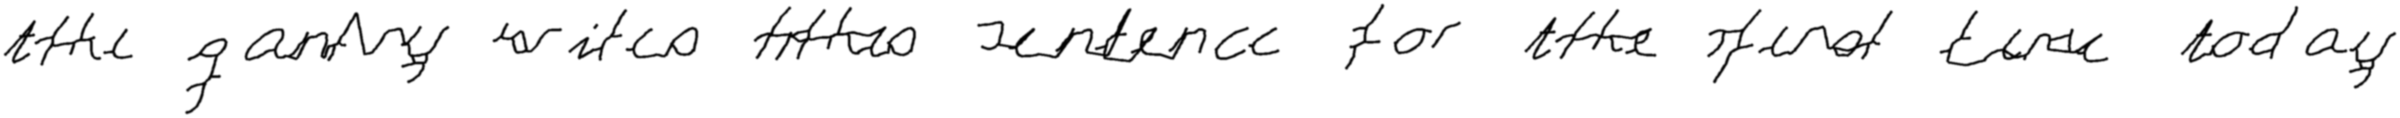
\includegraphics[width=0.95\linewidth]{Figures/w3_synth_153.png}
\caption{Synthesised line ``The gantry writes this sentence for the first time today'' for writer 150 (upper, printed hand; read back with three small errors) and writer 153 (lower, joined hand; read back as ``the garoby writes tttas senkence for tthe furst tuse today''), one seed and candidate each, rendered from the trajectory of an end-to-end run; the $N$ of that run was not recorded.}
\label{fig:syn-lines}
\end{figure}

\subsubsection{Design alternatives and justification}

A recurrent sequence generator with attention and mixture-density output needs on-line pen data, hundreds to thousands of lines per writer, whereas only 47 to 130 scanned lines per writer exist (Table~\ref{tab:sty-writers}); a from-scratch version trained on skeleton-derived strokes learned slant, roundness and connectedness but no legible letters and was rejected.
Adversarial and diffusion generators need less data through pre-training, but they emit a raster that needs the same thinning to vectorise, size, slant and spacing cannot be controlled as numbers, and a trial took 35 to 45\,s per line against 3 to 8\,s for glyph synthesis, so they were parked.
The glyph library needs about nine pages per writer and no training, outputs pen strokes directly, exposes size, slant, joins and gap as explicit numbers and has a traceable fallback for every glyph; synthesis itself costs about 15\,ms, so only the optional search is expensive, which suits a single-board computer without an accelerator, and the one weakness is joined hands, whose joins are lost by cutting.

\subsubsection{Known faults and limitations}
\label{sec:syn-faults}

\begin{enumerate}\setlength{\itemsep}{0pt}\setlength{\parskip}{0pt}
\item \emph{The legibility mechanism is inert as submitted.} \texttt{legibilityLambda} is absent from all thirteen stored profiles and \texttt{SynthesizeJointBestOf} defaults it to zero, so $\lambda=0$ on the live path: the second branch of Equation~\ref{eq:syn-swap} fires for every glyph below $d=0.55$, the \emph{only} substitutions left are the unconditional ones at $d\ge0.55$, and the cap stays at its widest, $\theta_{\mathrm{cap}}=45^\circ$. Every $\lambda$-dependent figure above, including the 0 to 76\,\% anchor share, describes the tuned configuration and \emph{not} the delivered one, and the outstanding tuner item of Section~\ref{sec:sty-faults} applies to all of them.
\item \emph{Every figure after the search was introduced is the opinion of the very networks that selected the output.} The search loads the same weight files as the measurement, so a best-of-$N$ search necessarily raises the score by which it is judged; the values show that the pipeline can satisfy its two judges, not that a human reader or an independent recogniser would agree.
\item $\lambda$, the anchor threshold and $N$ were tuned on the same sentences that Section~\ref{sec:results} measures.
\item The calibration of Equation~\ref{eq:syn-cal} measures both sides with the same estimator, so the agreement of slant and reach it achieves is partly self-fulfilling and is not independent evidence.
\item The repair pass updates the pin set only on acceptance, so after a rejection the next round re-synthesises an identical candidate and the remaining rounds are wasted work; in three probe runs, writers 150, 153 and 551 at $N=14$, no repair was accepted at all.
\item Three design-stage figures have no surviving raw log: the 80.5 against 75.5\,\% variant-restriction probe, the anchor-share probe, and the print skeleton's 96 and 84\,\% read-back, which exists only as a code comment.
\mustdo{the corresponding read-back accuracy of the \emph{cursive} skeleton. An earlier draft quoted about 89\,\% for it; that figure matches no comment or log in the delivered code and has been withdrawn rather than left standing as a measurement.}
\item Writers 151 and 552, the two most joined hands, reach only 53 and 56\,\% character accuracy through G-code against about 84\,\% for the other eleven, the clearest limitation of the exemplar approach.
\end{enumerate}


\subsection{G-code generation}
\label{sec:gcode}

This subsection describes how a trajectory in millimetres becomes a machine program (functional unit FU~2.8, first stage; requirements R3 and R5).
The format is G-code, the command language of plotters and numerically controlled machines standardised as ISO 6983-1~\cite{iso6983}. A G-code program is a list of text lines, each naming a command and its arguments. Only five commands are used here: \texttt{G21} and \texttt{G90} set the units to millimetres and the coordinates to absolute, \texttt{G0} is a move with the pen up and \texttt{G1} a move with the pen down, \texttt{M3} and \texttt{M5} lower and raise the pen, \texttt{G4} pauses, and \texttt{M2} ends the program.

Two conventions of the format matter to the design. Coordinates are \emph{absolute}, meaning each move names where to go rather than how far to move, so a rounding error in one move cannot accumulate into the next. Settings such as the feed rate are \emph{modal}, meaning a value stays in force until another line changes it, so the feed need not be repeated on every move. Fault~2 of Section~\ref{sec:gc-faults} is a consequence of that second convention being overlooked.

The format was chosen because it splits the motion chain in two. The generator needs to know nothing about the gantry electronics, the interpreter of Section~\ref{sec:gantry} needs to know nothing about handwriting, and the file between them is plain text that can be inspected and replayed without the machine being present, which is what makes the verification of Section~\ref{sec:gc-verify} possible at all. The generator was written for this project; the file format itself was not designed here and carries no design credit.

\subsubsection{Placement, ordering and program structure}

The trajectory of Section~\ref{sec:synthesis} and the machine frame both have $X$ to the right and $Y$ upwards, so no mirroring is needed.
The origin is the safe corner 5\,mm inside the minimum switches (Section~\ref{sec:gan-calib}), leaving the driver $194\times252$\,mm of the machine's $204\times262$\,mm switch-to-switch travel, and the text block starts at $(X_{\mathrm o},Y_{\mathrm o})=(10,180)$\,mm with later lines descending.
For a trajectory of bounding box $(x_0,y_0,x_1,y_1)$, width $w$ and height $h$, the block is shrunk by Equation~\ref{eq:gc-map}, never enlarged, if it would leave the work area $[0,X_{\max}]\times[0,Y_{\max}]$ with $X_{\max}=Y_{\max}=200$\,mm:
\begin{equation}
s=\min\Bigl(1,\ \frac{X_{\max}-X_{\mathrm o}}{w},\ \frac{Y_{\mathrm o}-Y_{\min}}{h}\Bigr),\qquad X=X_{\mathrm o}+(x-x_0)\,s,\quad Y=Y_{\mathrm o}-(y_1-y)\,s,
\label{eq:gc-map}
\end{equation}
with $Y_{\min}=0$; at scale 1 the area holds at most $\lfloor(180-9.2)/12.6\rfloor+1=14$ lines of the default size, where $9.2=(A-D)x_{\mathrm{mm}}$ and the pitch is 12.6\,mm.
A final clamp moves outlying vertices onto the border and writes a header warning, and vertices closer than 0.12\,mm to the previous one are dropped, which is inert in practice because the synthesiser resamples at 0.35\,mm.
The strokes are then ordered by a greedy nearest-endpoint rule, grouped into text rows and, within a row, the next stroke being the one whose end is nearest to the pen and entered from that end; only order and direction change, so the ink is identical, and this is the pen-movement optimisation of R3, with the row-order fault of Section~\ref{sec:gc-faults}.

The pen lift is a one-way toggle motor (Section~\ref{sec:gan-pen}), so the generator tracks the pen state in software and emits \texttt{M3} for down or \texttt{M5} for up only when the state changes, a pulse where none is needed inverting the pen for the rest of the job.
Each change is followed by a \emph{dwell}, which is a commanded pause that holds the machine still while something mechanical finishes. Here it covers one $90^\circ$ rotation of the cam and the settling of the pen afterwards, assumed to be $260+90=350$\,ms. A dwell is needed because the pen motor is not synchronised with the motion: without it, the next move would begin while the pen was still travelling, drawing a stroke that starts in the wrong place. Since every stroke needs the pen down and then up again, a stroke costs 0.7\,s of dwell, which is why dwell rather than drawing dominates the predicted job time. The interpreter additionally confirms the pen state with the pen switch rather than trusting the dwell alone.
A program is a comment header, \texttt{G21} for millimetres and \texttt{G90} for absolute coordinates, then one block per stroke of at least two points at the 900\,mm/min draw feed, and finally pen up, parking and \texttt{M2}, with vertices written to three decimals; Figure~\ref{fig:gc-emit} is the start of a generated program and Figure~\ref{fig:gc-emitpseudo} in Appendix~\ref{sec:app-sys} the loop that writes it.
Table~\ref{tab:gc-config} in the same appendix lists every constant with its role; the motor, driver and transmission values are assumptions made in the program comments, and the calibrated steps per millimetre of Section~\ref{sec:gan-calib} replace the derived ones in the interpreter, so a wrong assumption in the file header cannot reach the machine.

\begin{figure}[!htbp]
\centering
\fontsize{8}{9.2}\selectfont
\begin{lstlisting}[basicstyle=\ttfamily\fontsize{8}{9.2}\selectfont,frame=none]
; start of a generated program -- author yeukita
; steps/mm  X=80.000  Y=80.000 (3200 microsteps/rev)
G21   ; millimetres
G90   ; absolute
G0 F2400                     ; travel feed, emitted once
G0 X10.059 Y179.271          ; travel to the first stroke
M3   ; pen DOWN (one 90deg pulse of the one-way gear motor)
G4 P0.350   ; wait for the 90deg rotation to finish
G1 F900                      ; draw feed
G1 X10.084 Y178.920          ; one line per vertex (0.35 mm apart)
\end{lstlisting}
\caption{Start of a generated program for the test word of writer yeukita (14 strokes, 239 draw moves, vertices 0.348\,mm apart on average). The trailing comments on the motion lines are annotations added here. Every line of the format is accounted for: the two setting codes, one travel feed emitted once, a rapid move to the first point, the pen toggle with its dwell, the draw feed, and then one linear move per vertex. The loop that writes it is given as pseudocode in Appendix~\ref{sec:app-sys}.}
\label{fig:gc-emit}
\end{figure}


\subsubsection{Time model and verification}
\label{sec:gc-verify}

The generator can also write a step schedule with a time estimate, which assumes each move starts and ends at rest under the ramp that keeps an open-loop stepper from losing steps, with acceleration $a=400$\,mm/s$^2$ and cruise speed $v$, 15\,mm/s drawing and 40\,mm/s travelling.
The distance needed to reach $v$ is $d_a=v^2/(2a)$, so a move of length $d$ is \emph{trapezoidal} if $d\ge2d_a$ and otherwise \emph{triangular}, never reaching $v$ (Equation~\ref{eq:gc-trap}):
\begin{equation}
T(d)=\begin{cases}\dfrac{2v}{a}+\dfrac{d-2d_a}{v}=\dfrac{d}{v}+\dfrac{v}{a},&d\ge2d_a,\\[2mm]\dfrac{2v_{\mathrm p}}{a}=2\sqrt{\dfrac{d}{a}},\quad v_{\mathrm p}=\sqrt{d\,a},&d<2d_a.\end{cases}
\label{eq:gc-trap}
\end{equation}
For drawing $d_a=0.28$\,mm, so moves below 0.56\,mm are triangular with a 37.5\,ms ramp; for travel $d_a=2$\,mm, so moves below 4\,mm are triangular with 100\,ms.
A typical 0.35\,mm segment is therefore always triangular, with $T=2\sqrt{0.35/400}=59.2$\,ms, an average of 5.9\,mm/s and not 15.
For the test word of Figure~\ref{fig:gc-emit}, a draw path of 83.2\,mm in 239 moves and a pen-up path of 250.3\,mm in 14 moves with 26 pen pulses, the model gives 14.1\,s drawing, 7.5\,s travel and 9.1\,s dwell, 30.7\,s in all, or 2.8\,s per character for an assumed 11 characters, the text not being stored in the file.

The generator is the one stage whose output can be checked exactly, because both its input and its output are geometry and the correct answer is therefore known. The check is run by a second, independent parser that reads the finished file back as though it were the machine: it follows $X$ and $Y$, starts a polyline at \texttt{M3} and closes it at \texttt{M5}, and parses only \texttt{G0} and \texttt{G1} because nothing else is emitted. Writing a separate reader rather than reusing the generator's own data is the point of the exercise, since a fault shared by both would otherwise cancel out and go unseen.

The trajectory that went in and the polylines that come back out are then compared in two ways, in Equation~\ref{eq:gc-verify}.
\begin{equation}
\mathrm{IoU}=\frac{|M_{\mathrm t}\cap M_{\mathrm g}|}{|M_{\mathrm t}\cup M_{\mathrm g}|},\qquad e_{\mathrm{mean}}=\frac{1}{J}\sum_j\min_i\lVert g_j-s_i\rVert,\qquad e_{\max}=\max_j\min_i\lVert g_j-s_i\rVert
\label{eq:gc-verify}
\end{equation}
The first is an area comparison. Both are drawn onto a common grid of 8 pixels per millimetre, giving two masks $M_{\mathrm t}$ and $M_{\mathrm g}$, and the \emph{intersection over union} is the number of pixels inked by both divided by the number inked by either. It is 1 when the two drawings coincide exactly and falls towards 0 as they diverge, so it answers the question ``does the file draw the same picture'' with a single number. It is used rather than counting differing pixels because that count would depend on how much ink there is, whereas a ratio does not.

The second is a vertex comparison. For each vertex $g_j$ of the G-code, the distance to the nearest vertex $s_i$ of the original trajectory is found, and the mean and the worst of those distances are reported. The mean shows whether the whole drawing has shifted and the maximum catches a single vertex that has moved, which an area measure would hide because one misplaced point changes almost no pixels. The vertices are sub-sampled to at most 4000 and 6000 respectively to keep the all-pairs search affordable.

What Equation~\ref{eq:gc-verify} does and does not cover should be clear. It measures only the loss between the trajectory and the file, which is rounding to three decimals, the stroke reordering and the clamping to the work area. It says nothing about whether the machine then draws the file correctly, which is the mechanical error of Section~\ref{sec:gan-res} and a separate matter entirely.

\subsubsection{Known faults and limitations}
\label{sec:gc-faults}

\begin{enumerate}\setlength{\itemsep}{0pt}\setlength{\parskip}{0pt}
\item The stroke rows are sorted by ascending $Y$, so a multi-line job starts with the \emph{bottom} line and not in reading order; this was found by reading the code and was not checked on the machine.
\item The interpreter has one \emph{modal} feed register and no rapid mode (Section~\ref{sec:gantry}), but the generator emits \texttt{G0 F2400} once at the start and \texttt{G1 F900} before every stroke, so every pen-up travel after the first stroke runs at 900\,mm/min and not 2400; the real job time is therefore longer than the time model assumes, and emitting the feed before every travel would remove the discrepancy.
\item Lines wrap at 185\,mm from $X_{\mathrm o}=10$\,mm, so a full-width line reaches $X=195$\,mm, but the driver clamps $X$ to 194\,mm and would distort the last millimetre; $X_{\max}$ or the line width should be reduced.
\item Equation~\ref{eq:gc-trap} is a model and not a measurement: it stops fully between 0.35\,mm segments and assumes 40\,mm/s travel, so it overestimates drawing time and underestimates travel time against the real interpreter (Section~\ref{sec:gan-timing}).
\item Equation~\ref{eq:gc-verify} compares vertices with vertices, so it covers only the loss between trajectory and file, namely rounding, ordering and clamping, and not the mechanical error (Section~\ref{sec:gan-res}). The project notes quote $\mathrm{IoU}\approx0.99$ and a text-accuracy change of at most 0.3 percentage points between direct and read-back rendering, for an earlier system state and judged by the networks of the search (Table~\ref{tab:syn-evid} shows later pairs); $e_{\mathrm{mean}}$ and $e_{\max}$ were never logged.
\mustdo{run the comparison for a set of generated programs and report $\mathrm{IoU}$, $e_{\mathrm{mean}}$ and $e_{\max}$.}
\item The saving produced by the stroke-ordering optimisation of R3 was not measured.
\end{enumerate}


\subsection{Modifications made after the chain could be measured}
\label{sec:later}

The subsections above describe each subsystem as delivered. Four of those designs are not what was built first: they replaced an earlier version once the complete chain existed and the output could be measured end to end, which is the point at which faults invisible inside a single subsystem became apparent. They are collected here because each was a change of approach rather than a correction of code, and because the reason for each lies outside the subsystem it altered.

\subsubsection{A second writer classifier, judging shape instead of ink}
\label{sec:later-strokenorm}

The first writer classifier was trained on grey-scale crops and read real held-out lines at 99.78\,\% over 1358 lines, which satisfied requirement R2 on photographed pages. Measured on \emph{synthesised} output, however, the same classifier identified the intended writer in only about 28\,\% of trials. The cause is a property of the machine rather than of the network: the gantry draws every stroke with one pen at one width and one pressure, whereas real handwriting carries a thickness and an ink density that a convolutional network exploits readily when the training lines are few. A classifier that leans on those cues therefore predicts neither what the machine can draw nor how a reader recognises a hand, which is by geometry.

The response was to train a second classifier of the same architecture on stroke-normalised crops, in which the ink is thinned to a centre line and redrawn at a constant width proportional to the letter height, so thickness is removed by construction (Section~\ref{sec:wid-strokenorm}). The two are used for different purposes, and the division is kept throughout the system: the ink classifier serves real photographed pages, and the shape classifier serves the candidate search of Section~\ref{sec:syn-search}. Neither replaced the other, so the writer-identification block carries two sets of weights rather than one.

\subsubsection{End-to-end training in place of a frozen backbone}
\label{sec:later-endtoend}

The shape classifier was first trained by fitting only the 13\,645 parameters of its head on feature vectors extracted once from a frozen backbone. That recipe is a training fault for the reason given in Section~\ref{sec:writerid}: because the features were extracted once, no augmentation was re-sampled between epochs and every line contributed the same four fixed vectors for all 500 epochs. Training all 966\,445 parameters end to end instead raised the same measurement from 83.36\,\% to 93.67\,\% on the same 1358 real lines, and removed a failure in which 118 of one writer's 148 lines had been assigned to a single neighbour. Every figure quoted for the shape classifier elsewhere in this report is from the end-to-end model; the frozen-head figures describe the superseded one.

\subsubsection{Selecting a candidate on both criteria instead of legibility alone}
\label{sec:later-joint}

The candidate search first kept whichever of the $N$ draws the text recogniser read most accurately. That raised legibility and, for some writers, lowered writer identification, because the most legible of several random draws has no reason also to be the most characteristic. The score was therefore changed to the harmonic mean of the recogniser's character accuracy and the shape classifier's confidence in the intended writer, Equation~\ref{eq:syn-score}, which is dominated by whichever of the two is smaller and so cannot be won on one criterion while failing the other. The repair loop was changed in the same way and for the same reason, accepting a repaired line only when the joint score improves, so that a repair which fixes a letter but makes the line resemble another writer is rejected rather than taken. The evidence for both changes is in Table~\ref{tab:syn-evid}.

\subsubsection{Line-level style calibration}
\label{sec:later-cal}

Glyphs are stored and placed one instance at a time, so a line assembled from them does not reproduce the writer's line-level slant and ascender reach automatically. The calibration of Section~\ref{sec:syn-cal} was added to correct that drift, measuring a rendered probe with the same functions that measured the writer's real pages and returning a shear and reach correction. The drift it corrects was itself measured before the change: writer 150's ascenders came out about 7\,\% too tall and writer 551's slant about $9^\circ$ too steep against their own real lines (Section~\ref{sec:syn-cal}).
Its effect after the change differs between the two judges, and the shape classifier was taken as the one that predicts the physical machine, since the machine writes every writer with the same pen.
Unlike the other three changes, this one has no before-and-after pair in Table~\ref{tab:syn-evid}, so its benefit rests on the probe agreeing with the stored reference rather than on a judge's score, and item~4 of Section~\ref{sec:syn-faults} records why that agreement is partly self-fulfilling.
\mustdo{measure writer identification and character accuracy with the calibration of Equation~\ref{eq:syn-cal} disabled and enabled, over the same sentences and seeds as the other rows of Table~\ref{tab:syn-evid}, so that this change carries the same kind of evidence as the other three.}

\mustdo{confirm that these four are the complete set of changes of approach, and add any others that belong here --- for example a change to the segmentation thresholds, to the number of writers, or to the requirement allocation --- each with what was measured before and after.}


\subsection{Software design and system integration}
\label{sec:system}

% Compact display spacing for this subsection only; restored at the end of the file.
\begingroup
\setlength{\abovedisplayskip}{4pt}\setlength{\belowdisplayskip}{4pt}
\setlength{\abovedisplayshortskip}{2pt}\setlength{\belowdisplayshortskip}{2pt}

This subsection describes how the blocks of Sections~\ref{sec:gantry} to~\ref{sec:later} form one application on the single-board computer, which runs a web server exposing them to a browser. All are Python programs written for this project; only the camera interface, the pin interface and the transport of web requests come from libraries, with the one exception below.

\subsubsection{Process flow and start-up}

Figure~\ref{fig:sys-flow} is the process flow of the two run-time modes. At start-up the application loads the thirteen profiles and the three networks, each a from-scratch array-arithmetic evaluation of trained weights (Sections~\ref{sec:textrec} and~\ref{sec:writerid}); the reproduction chain then calls the synthesiser once with both judges passed in and refuses to send unless calibration has succeeded in this session. Training is a third mode, the writers being pre-built files from offline programs. \mustdo{the board's address and connection to the laptop, the operating system and Python version, how the server is started, and the memory the loaded models use.}

\begin{figure}[!htbp]
\centering
\begin{tikzpicture}[x=1cm,y=1cm]
\tikzset{p/.style={w3box,text width=2.2cm,minimum height=1.0cm,font=\scriptsize},
         s/.style={w3store,text width=2.2cm,minimum height=0.85cm,font=\scriptsize},
         i/.style={w3io,text width=2.2cm,minimum height=0.85cm,font=\scriptsize}}
\node[p] (a1) at (0,0) {Read page: capture or upload};
\node[p] (a2) at (3,0) {Condition, segment lines};
\node[p] (a3) at (6,0) {Recogniser and ink classifier};
\node[p] (a4) at (9,0) {Mean writer probabilities};
\node[p] (a5) at (12,0) {Text, writer, confidence};
\node[p] (b1) at (0,-1.9) {Write page: text, writer, $N$};
\node[p] (b2) at (3,-1.9) {Best-of-$N$ synthesis};
\node[p] (b3) at (6,-1.9) {G-code and preview};
\node[p] (b4) at (9,-1.9) {Read-back by recogniser};
\node[p] (b5) at (12,-1.9) {Send to calibrated gantry};
\node[s] (prof) at (3,-3.25) {Thirteen style profiles (JSON)};
\node[i] (gan) at (12,-3.25) {Gantry, pen, switches};
\begin{scope}[on background layer]
\node[w3group,fit=(a1)(a5)(b1)(b5),inner sep=7pt] (srv) {};
\end{scope}
\node[font=\scriptsize\bfseries,anchor=south west] at (srv.north west) {One application on the ODROID N2+};
\foreach \u/\v in {a1/a2,a2/a3,a3/a4,a4/a5,b1/b2,b2/b3,b3/b4,b4/b5} \draw[w3arr] (\u) -- (\v);
\draw[w3arr] (prof) -- (b2);
\draw[w3arr] (b5) -- (gan);
\end{tikzpicture}
\caption{Process flow of the two run-time modes: classification above, reproduction below, the writer the upper chain identifies being what the lower chain is given. The profile builder of Section~\ref{sec:styleprofile} is offline and appears in neither.}
\label{fig:sys-flow}
\end{figure}

\paragraph{The inference path is library-free; the sample-crop warm-up is not.}
A recorded cold-boot import closure confirms that \texttt{torch}, \texttt{scipy}, \texttt{cv2} and \texttt{tensorflow} are reached by none of the three networks and none of the classification, synthesis, G-code and motion paths: every weight comes from a plain array archive and every layer is evaluated by the project's own array arithmetic. One path breaks that. The start-up warm-up, given as pseudocode in Figure~\ref{fig:sys-code-warm}, calls \texttt{WRH.SampleCrops} for every writer, and on a cache miss that helper imports \texttt{BuildStyleProfile}, \texttt{TrainAuthor} and \texttt{TrainText}; \texttt{WebRenderHelpers.py} prepends \texttt{Software/CNN} and its \texttt{AuthorReproductionStuff} to \texttt{sys.path}, so those names resolve to the \emph{retired} tree, whose \texttt{TrainText.py} and \texttt{TrainAuthor.py} import \texttt{torch}, \texttt{torchvision}, \texttt{pytesseract} and \texttt{scipy} at module level. \texttt{WebCache} as delivered has no glyph grid or crops for owen and thiya and none for abhinav, so the miss, and the import, happen on \emph{every} start. \mustdo{port the two sample-crop helpers into \texttt{CleanPipeline}, or pre-populate \texttt{WebCache} for owen, thiya and abhinav, so that no import reaches \texttt{Software/CNN}; then repeat the cold-boot closure on the board.}


\paragraph{Known inconsistency: the stored accuracy figures.}
One route computes nothing: it returns figures hard-coded in \texttt{Server.py}, several no longer agreeing with Section~\ref{sec:results} --- the ink-based classifier at 100.0\,\%, the stroke-normalised one at 96.7\,\% on real ink and 99.2\,\% on synthesised output, the recogniser at 89.4\,\% on real ink, and the pipeline at 99.2\,\% writer identification with 85.8\,\% and 84.1\,\% character accuracy direct and through G-code. The code is stale here, not the report, and the page displaying those figures contradicts the Results chapter. \mustdo{update the hard-coded accuracy block of \texttt{/api/model\_info} to the final figures of Section~\ref{sec:results}, or have the route read them from the evaluation output.}

\subsubsection{Timing chains of the two modes}

Requirement R4 limits the classification of $x$ characters by Equation~\ref{eq:sys-cls},
\begin{equation}
T_{\mathrm{cls}}=T_{\mathrm{cap}}+T_{\mathrm{seg}}+\sum_{\mathrm{lines}}\bigl(T_{\mathrm{text}}+T_{\mathrm{wid}}\bigr)\le2\ \mathrm{s}+0.025\,x\ \mathrm{s},
\label{eq:sys-cls}
\end{equation}
leaving both network passes 25\,ms per character, and R3 limits reproduction by Equation~\ref{eq:sys-rep},
\begin{equation}
T_{\mathrm{rep}}=T_{\mathrm{synth}}+T_{\mathrm{gcode}}+T_{\mathrm{motion}}\le4\,x\ \mathrm{s},\qquad T_{\mathrm{synth}}\approx N\,C,
\label{eq:sys-rep}
\end{equation}
with $C$ the cost of one candidate (Equation~\ref{eq:syn-cost}), $T_{\mathrm{gcode}}$ in milliseconds and $T_{\mathrm{motion}}$ the job time of Section~\ref{sec:gan-timing}; the calibration is excluded and $T_{\mathrm{synth}}$ included, the stricter reading of the proposal.
A budget is only a design once it is apportioned, and Table~\ref{tab:app-budget} in Appendix~\ref{sec:app-sys} gives the allowance this design assigned to each stage of Equations~\ref{eq:sys-cls} and~\ref{eq:sys-rep} against the figure later measured for it.
The apportionment follows from the structure of the chain rather than from the measurements: the two network terms were given the whole per-character allowance of R4, being the only terms that grow with $x$, which leaves the fixed two seconds for capture, conditioning and segmentation; and in R3 the physical writing was given three quarters of the per-character allowance, being the one term that no faster computer can reduce.
Read against that apportionment, four of the five stages are inside their allowance and the whole R4 shortfall sits in page segmentation, at twelve to thirty-five times what it was allowed.
Table~\ref{tab:sys-timing} lists the stages, and \emph{no stage was timed on the single-board computer}: a 56-character sentence allows 224\,s, while the search alone took 23 to 137\,s at $N=14$ on the laptop and the motion model gives 2.4 to 2.8\,s per character, so R3 and R4 are not claimed to be met. \mustdo{the timings of the stages on the single-board computer, listed in Table~\ref{tab:sys-timing}.}

\begin{table}[!htbp]
\centering
\fontsize{8}{9.3}\selectfont
\setlength{\tabcolsep}{3.5pt}\renewcommand{\arraystretch}{1.02}
\begin{tabularx}{\linewidth}{|p{3.2cm}|X|}
\hline
\textbf{Stage} & \textbf{Known information and value to be supplied} \\
\hline
Capture, conditioning and segmentation & Framing by the user, five discarded frames without preview; whole page on the board. \mustdo{time from pressing capture to the stored image.} \mustdo{conditioning and segmentation time per page on the board.} \\
\hline
Recognition and writer classification & Two passes of about $4\times10^9$ multiply--accumulate operations per line. \mustdo{time per line on the board and the total for the R4 test paragraph.} \\
\hline
Synthesis, G-code and preview & Synthesis time is returned in the server response (laptop values in Table~\ref{tab:syn-cost}); the generator and preview are milliseconds, not measured. \mustdo{synthesis time on the board for the $N$ used in the demonstration.} \\
\hline
Gantry motion & Model 2.4 to 2.8\,s per character (Section~\ref{sec:gan-timing}). \mustdo{stopwatch time of a sentence of known length, from send to the final pen lift.} \\
\hline
\end{tabularx}
\caption{Stages of the timing chains of the two modes and the measurements still missing.}
\label{tab:sys-timing}
\end{table}

Complete code has been submitted separately on the AMS.
\mustdo{confirm which archive and revision was submitted on the AMS.}

\endgroup

